\documentclass[12pt,fleqn]{report}
\usepackage{color}
\usepackage{multicol}
\usepackage{makeidx}
\usepackage{bm}
\makeindex

\usepackage[linkbordercolor={0 0 1}]{hyperref}
\usepackage[pdftex]{graphicx}

\definecolor{light-gray}{gray}{0.95}

\newcommand{\keyword}[1]{\index{Keywords!{\tt #1}} {\tt #1}}
\newcommand{\cv}[1]{\index{Collective variables!{#1}}
\index{{#1}|see{Collective variables, {#1}}} }
\newcommand{\plumed}{{\tt PLUMED}}


\newcommand{\esempio}[1]{
\vspace{10pt}
\begin{flushright}
\colorbox{light-gray}{
   \begin{minipage}{13cm}
       \scriptsize{
{\fontfamily{phv} \fontseries{b}
 \selectfont Example. \\
 \fontseries{m} \selectfont #1 } }
\end{minipage}}
\end{flushright}
\vspace{20pt}
}

\begin{document}

%% -----------------------------------------------------------------------------------------
\begin{titlepage}
\vspace{4cm}
\begin{flushleft}
{
 { \fontencoding{OT1}\fontfamily{phv} \fontshape{i} \fontseries{b} \Huge{PLUMED Tutorial}} \\ \vspace{.5cm}
 { \fontencoding{OT1}\fontfamily{phv} \fontshape{sl} \selectfont \Large{A portable plugin for free-energy calculations \\ with  molecular dynamics}}
}
\rule{12cm}{4pt}
\end{flushleft}
\vspace{1cm}
\begin{figure}[here!]
\begin{center}
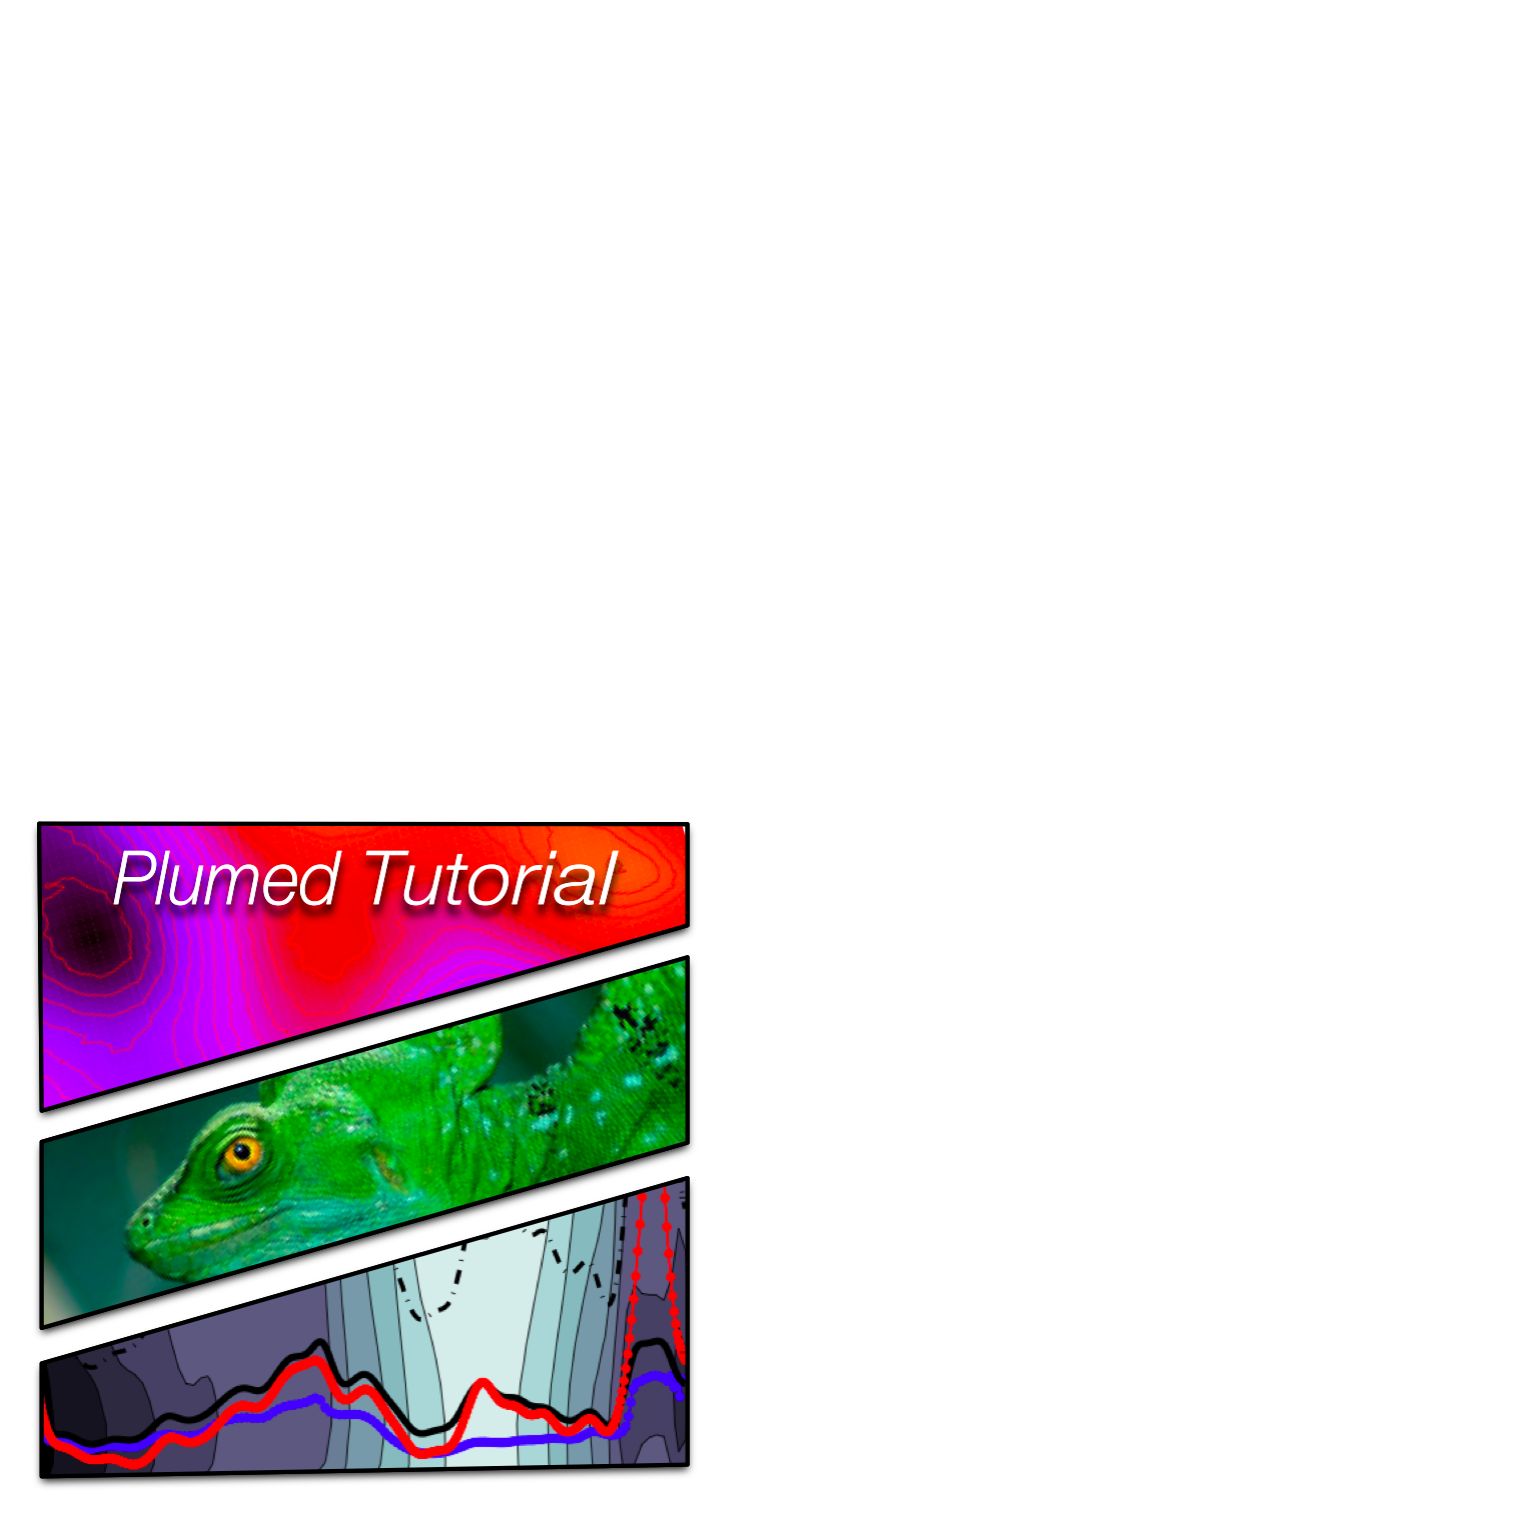
\includegraphics[width=10cm,angle=0]{./figures/symbol}
\end{center}
\end{figure}
\vspace{1cm}
\begin{flushright}
 \fontencoding{OT1}\fontfamily{phv} \fontseries{b} \fontshape{i} \large{CECAM, Lausanne, Switzerland} \\
 \fontencoding{OT1}\fontfamily{phv} \fontseries{b} \fontshape{i} \large{September 28, 2010 - October 1, 2010}
\end{flushright}
%% -----------------------------------------------------------------------------------------



\end{titlepage}

\newpage

\noindent
\large{This document and the relative computer exercises have been written by:}\\ \\
\Large{Massimiliano Bonomi\\ Davide Branduardi\\ Giovanni Bussi\\ 
Francesco Gervasio\\ Alessandro Laio\\ Fabio Pietrucci}\\ \\ \\ \\
\large{
Tutorial website:\\
{\tt http://sites.google.com/site/plumedtutorial2010/}\\ \\ 
PLUMED website:\\
{\tt http://www.plumed-code.org}\\ \\ 
PLUMED users Google group:\\
{\tt plumed-users@googlegroups.com}\\ \\ 
PLUMED reference article: \\ 
M.~Bonomi, D.~Branduardi, G.~Bussi, C.~Camilloni, D.~Provasi, P.~Raiteri,
D.~Donadio, F.~Marinelli, F.~Pietrucci, R.A.~Broglia and M.~Parrinello,
\href{http://dx.doi.org/10.1016/j.cpc.2009.05.011}{PLUMED: a portable plugin for free-energy calculations with molecular dynamics},
 Comp.~Phys.~Comm. 2009 vol. 180 (10) pp. 1961-1972.
}

\newpage

\tableofcontents

\chapter{Compilation}

\section{PLUMED compilation}
\label{installgromacs}
Here in the following we will show a bunch of codes that work with plumed.
They have been chosen because they are all free codes and can be downloaded straight from the web without any 
license or agreement. FIrst we will show a classical code and secondly an ab-initio code.
First some useful informations.
You log in as user {\tt tutoXX } (which stands for {\tt tuto01},{\tt tuto02} etc...). You will be assigned a node,  say {\tt nodeYYY}.
All the tests should be run in the node.
Therefore you have open a terminal and access the node you have been assigned
\begin{verbatim}
ssh -X tutoXX@nodeYYY
\end{verbatim} 
and you are on the node.
Change to the scratch directory
\begin{verbatim}
cd /scratch
\end{verbatim} 
If the directory {\tt tutoXX} does not exist create it and enter it.
\begin{verbatim}
mkdir tutoXX
cd tutoXX
\end{verbatim} 
This is the place where you will run all the calculations.
You have a maximum of {\bf{\underline{4 processors per terminal}}}. You will see later how to use them.
All the exercises will be provided daily and you may find them into:
\begin{verbatim}
/nfs_home/tutoadmin/PLUMED/EXERCISES_FINAL
\end{verbatim} 
which are accessible read-only.
You will find the directories
\begin{verbatim}
1_compiling  2_basics  3_biasing ...
\end{verbatim} 
and you will be told time to time which directory you should copy into your {\tt /scratch/tutoXX} directory for the exercise as indicated by the tutor.
Now copy the directory into your scratch
\begin{verbatim}
cd /scratch/tutoXX
cp -r /nfs_home/tutoadmin/PLUMED/EXERCISES_FINAL/1_compiling .
\end{verbatim}
The documentation (a file {\tt tutorial.pdf} with the practical lessons and the slides) are put in
\begin{verbatim}
/nfs_home/tutoadmin/PLUMED/DOCUMENTATION
\end{verbatim} 
and updated daily (and bugs solved: help us in improving it!). Check it from time to time when the tutor tells you.

Now let'us go back to the compiling: first enter the {\tt 1\_compiling/plumed} directory and untar \plumed\
\begin{verbatim}
cd 1_compiling/plumed
tar -zxvf PLUMED-1.2.1.tar.gz
cd ../
\end{verbatim}
 
\subsection{Compile \plumed\ with GROMACS}
In this section we will discuss how to compile plumed in the CECAM machine.
Our "reference" code is GROMACS (version 4.0.7) but other versions works in identical way.
Please note that, as the number of codes supported by \plumed\ is getting larger, we're trying at least 
to discontinue the old version of the code (version 3.3 in GROMACS).

What you need to compile a GROMACS version 4.0.7 on the {\tt ottokar} cluster at cecam is similar to what you 
generally need on a standard Linux machine.
\begin{itemize}
\item c/c++ compilers are available (gcc/g++ are fine. Intel compilers on Linux boxes are also free for academic). We assume this is already installed on the machine as many Linux suites allow to download them directly as rpm packages.
\item FFTW fast fourier libraries \url{http://www.fftw.org/}. 3.2.2 version is working nicely for most of cases. We assume this to be already installed on the system.
\item Message Passing Interface (MPI) is installed (Openmpi or MPICH are freely available from \url{http://www.open-mpi.org/}). In several Linux distros you can download it as rpm packages so we assume this to be available on your system.
\item GROMACS package (4.0.7) for this example (see  \url{http://www.gromacs.org}).
\item \plumed\ distribution is available (probably at this stage you will have a 1.2.1 version) at the usual website \url{http://www.plumed-code.org}.
\end{itemize}

The installation procedure closely follows the GROMACS installation with the exception that, between configuration step and compilation, you have to apply \plumed\ patch. Let us revise step-by-step the procedure you have to carry out and let us assume that we work with a \underline{bash shell} so that we set up variables accordingly.

First let's start by installing the serial version (double precision) and then we will proceed in installing the parallel version of mdrun.
First we move to the installation directory of the exercises. We should have everything we need.
We will make use of the Intel compilers here. Generally, neglecting the specific compiler variables, the default should be gcc.
On {\tt ottokar} cluster and on many HPC machines most of the useful environment variables are automatically provided via the {\tt module} command.
%\begin {verbatim}
%myuser> module available
%myuser> module load intel-cc/10.1.015
%myuser> icc 
%myuser> module unload intel-cc/10.1.015
%myuser> icc 
%\end{verbatim}
\begin {verbatim}
myuser> module load intel-cc/10.1.015 
myuser> module load fftw/3.2.2_intel-10.1.015
\end{verbatim}
and we can conveniently set up some variables that we will use and reuse at runtime
\begin {verbatim}
myuser> fftw=/opt/fftw-3.2.2/intel-10.1.015
myuser> mycc=icc
myuser> myld=icc
myuser> mycxx=icpc
myuser> cd gromacs
myuser> mydir=`pwd`
\end{verbatim}
Now we can unpack the GROMACS code and enter it. We also create a directory {\tt install\_dir} where all the final
installation will be placed. It is rather convenient that you create your custom installation directory so you don't affect the installation 
of the other users (probably you'll be prevented to do this in any case, unless you do the installation as root user).
\begin {verbatim}
myuser> tar -zxvf gromacs-4.0.7.tar.gz
myuser> cd gromacs-4.0.7
myuser> mkdir install_dir
\end{verbatim}
Now we proceed with the full configuration:
\begin {verbatim}
myuser>./configure LDFLAGS=-L${fftw}/lib 
         CPPFLAGS=-I${fftw}/include 
         --prefix=$mydir/gromacs-4.0.7/install_dir 
         CC=$mycc LD=$myld 
         CXX=$mycxx --with-fft=fftw3  
         --disable-float --program-suffix=_d
\end{verbatim}
Let us analyze what is done in this command. It first tells the {\tt configure} utility where to get the fftw through the {\tt LDFLAGS} and {\tt CPPFLAGS}.
Then it tells where the final installation should be done( {\tt --prefix=\$mydir/gromacs-4.0.7/install\_dir}). This is the location where you
will find libraries, executables, includefiles, manuals and topologies for gromacs. The {\tt CC,LD,CXX} specify the compiler you intend to use.
In this case it will be Intel compilers. If you omit this the default gcc compiler will be used. 
The flag {\tt --disable-float } specify to compile GROMACS in {\underline in double precision which is highly recommended for a correct \plumed\ intallation} .
Then the {\tt --program-suffix=\_d } specifies that all the executables will have the suffix \_d and this is needed so you know that the executables
you use are double precision by default.
Now it come the patching procedure itself. You first have to specify the \plumed\ location by setting the environment variable {\tt plumedir}.
\begin{verbatim}
myuser> export plumedir="my/path/to/plumed"
myuser> chmod +x $plumedir/patches/plumedpatch_gromacs_4.0.4.sh
myuser> $plumedir/patches/plumedpatch_gromacs_4.0.4.sh -patch
\end{verbatim}
where {\tt my/path/to/plumed} will look something like {\tt /scratch/tutoXX/1\_compiling/plumed/PLUMED-1.2.1}
Then have a look to what is happening. If the patching procedure goes fine you should have something like this.
\begin{verbatim}
* I will try to patch PLUMED version cvs ...
-- Executing pre script
-- Setting up symlinks
-- Setting up recon symlinks
-- Applying patches
patching file ./src/kernel/md.c
patching file ./src/kernel/repl_ex.c
Hunk #4 succeeded at 204 (offset 4 lines).
Hunk #5 succeeded at 220 (offset 4 lines).
Hunk #6 succeeded at 452 (offset 4 lines).
Hunk #7 succeeded at 481 (offset 4 lines).
Hunk #8 succeeded at 511 (offset 4 lines).
Hunk #9 succeeded at 569 (offset 4 lines).
Hunk #10 succeeded at 613 (offset 4 lines).
Hunk #11 succeeded at 682 (offset 4 lines).
patching file ./src/kernel/repl_ex.h
patching file ./src/kernel/Makefile
patching file ./src/kernel/mdrun.c
-- Executing post script
- DONE!
\end{verbatim}
If you find some failures at this stage it is likely that the GROMACS download version changed somehow or you choose the wrong
patch for this code. Please note that a successful patching does not mean a successful compiling. So please check carefully if you have errors during the compiling after the
patching is done.

Now you are ready. Give it a go!
\begin{verbatim}
myuser> make 
myuser> make install
\end{verbatim} 
Check that you have everything you need:
\begin{verbatim}
myuser> ls install_dir/bin
\end{verbatim} 
Now, assuming everything went fine, let us recompile {\tt mdrun} only in double precision, with MPI support.
First, let us clean and unpatch:
\begin{verbatim}
myuser> make clean  
myuser> $plumedir/patches/plumedpatch_gromacs_4.0.4.sh -revert
\end{verbatim} 
Load the parallel compilers:
\begin{verbatim}
myuser> module load openmpi/1.2.6_intel-10.1.015
\end{verbatim} 
and now we can reconfigure and repatch:
\begin{verbatim}
myuser> ./configure LDFLAGS=-L${fftw}/lib 
         CPPFLAGS=-I${fftw}/include 
         --prefix=$mydir/gromacs-4.0.7/install_dir 
         CC=$mycc LD=$myld 
         CXX=$mycxx --with-fft=fftw3  
         --disable-float --program-suffix=_mpid
         --enable-mpi 
myuser> $plumedir/patches/plumedpatch_gromacs_4.0.4.sh -patch
myuser> make mdrun
myuser> make install-mdrun
\end{verbatim} 
Verify once again that everything went fine in patching and compilation.
Now in the {\tt install\_dir/bin} directory you should have all the {\tt *\_d} executable and 
{\tt mdrun\_mpid} which you just compiled.
Now, for having all the executables in your path you have to source GMXRC
\begin{verbatim}
myuser>source ./install_dir/bin/GMXRC
\end{verbatim}
and now {\tt mdrun\_d} and  {\tt mdrun\_mpid} should be in your path.
Just chek it by doing
\begin{verbatim}
myuser>mdrun_d
myuser>mdrun_mpid
\end{verbatim}
should work and GROMACS should print out its banner and die (no input file provided).
\subsection{Compile \plumed\ with QUANTUM ESPRESSO}
Here we show how to compile \plumed\ with the popular DFT package QUANTUM ESPRESSO (\url{http://www.quantum-espresso.org}) on the 
CECAM machine {\tt ottokar}.
Actual version of QUANTUM ESPRESSO is 4.2.1 and the plumed patch for version 4.2 works fine for the 4.2.1 version as well.
First we load the environments for the Intel compilers and openmpi intel compilers.
Now enter the directory {\tt 1\_compiling/quantumespresso} and do
\begin{verbatim}
myuser> module purge
myuser> module load intel-cc/10.1.015 
myuser> module load intel-fc/10.1.015
myuser> module load intel-mkl/10.0.1.014 
myuser> module load openmpi/1.2.6_intel-10.1.015
\end{verbatim} 
Then we unpack the code and simply configure.
\begin{verbatim}
myuser> tar -zxvf espresso-4.2.1.tar.gz 
myuser> cd espresso-4.2.1
myuser> ./configure 
\end{verbatim} 
This should provide the basic configuration to install the clean QUANTUM ESPRESSO package.
\begin{verbatim}
myuser> export plumedir="my/path/to/plumed"
myuser> chmod +x ${plumedir}/patches/plumedpatch_qespresso_4.2.0.sh
myuser> ${plumedir}/patches/plumedpatch_qespresso_4.2.0.sh -patch
myuser> make pw
\end{verbatim} 
As usual, check if the patch produce any error. 
After few minutes you should have obtained a version of pw (you should have {\tt ./bin/pw.x}) that is ready and working.
\subsection{Compile \plumed\ with LAMMPS}
Another interesting classical molecular dynamics code is LAMMPS. LAMMPS  is a very scalable code intended primarily for 
solid state and mesoscopic simulations. It includes a variety of force field and functional forms and is fully customizable via
an interface that allows you to accept/reject plumed as an addon to the code. You may download it from \url{http://lammps.sandia.gov} free of charge.
Compiling LAMMPS can be non trivial and here we assume to do a very basic installation where the main flags have been setted up
for the {\tt ottokar} machine.

First, goto into the directory containing LAMMPS and untar it and load the modules that then you will need for compiling. 

\begin{verbatim}
myuser> cd 1_compiling/lammps
myuser> tar -xvf lammps.tar.gz
myuser> cd lammps-24Sep10
myuser> module purge
myuser> module load intel-cc/10.1.015
myuser> module load intel-fc/10.1.015 
myuser> module load fftw/2.1.5_intel-10.1.015    
myuser> module load openmpi/1.2.6_intel-10.1.015 
\end{verbatim}
Now copy some Makefiles that have been specifically hacked to work on the machine you are using
\begin{verbatim}
myuser> cp  ../Makefile.icc.atc ./lib/atc/Makefile.icc
myuser> cp ../Makefile.openmpi ./src/MAKE/Makefile.openmpi  
\end{verbatim}
The very first thing one should do is to compile the modules that appears in the lib directory and that one intend to compile (all these 
Makefiles have been suitably hacked to run on the {\tt ottokar} machine ):
\begin{verbatim}
myuser> cd  ./lib/atc
myuser> make -f Makefile.icc
myuser> cd ../meam
myuser> make -f Makefile.ifort
myuser> cd ../poems
myuser> make -f Makefile.icc
myuser> cd ../reax
myuser> make -f Makefile.ifort
myuser>  cd ../../
\end{verbatim}
These modules are additional packages that must compiled as libraries and you might need. We just skip the gpu package as 
we intend to use the code on a standard CPU based machine.
At this stage you are ready for compiling the clean version and you should edit the most appropriate {\tt Makefile.arch} in the {\tt ./src/MAKE} directory.
In {\tt ottokar} we use the {\tt Makefile.openmpi} configuration file suitably adapted in  few things (location of FFTW, location of Intel compilers libraries)
that we will provide along with the installation. Overwrite it on {\tt ./src/MAKE/Makefile.openmpi} and you are done.
Next step is patching the code  as usual
\begin{verbatim}
myuser>  export plumedir="my/path/to/plumed"
myuser> chmod +x ${plumedir}/patches/plumedpatch_lammps_24-09-2010.sh
myuser>  ${plumedir}/patches/plumedpatch_lammps_24-09-2010.sh -patch
\end{verbatim}
At this stage we should have everything we need and we should proceed to a standard LAMMPS installation.
We first install the modules we need
\begin{verbatim}
myuser> cd src
myuser> make yes-standard
myuser> make no-gpu
\end{verbatim}
and check if \plumed\ is already turned on (it should be done automatically by the patching procedure).
\begin{verbatim}
myuser> make  package-status
...
Installed YES: package USER-PLUMED
...
\end{verbatim} 
Now simply do:
\begin{verbatim}
myuser> make openmpi
\end{verbatim}
and after some ages(!) you should get the executable {\tt lmp\_openmpi}.

\chapter{Basics: monitoring simulations}

In this chapter we will see the basics instruction for creating a \plumed\ input files and review the output that it produces during the 
simulation. At the end of this chapter the user should be able to write a simple plumed input file and monitor the CVs of choice by simply 
consulting the manual for each CV individual syntax. The philosophy behind \plumed\ requires 
that one may use the same input with different programs.
This is only partly true because different programs have different internal units. For example, in GROMACS, distances are in nm and energies are 
in kjoule/mol while in NAMD and SANDER the distances are in $\rm \AA$ and the energies are in kcal/mol. Keep this in mind because it is crucial to understand which are the internal units of the program you are running before you do a simulation. It may let you save lots of human and computer time. Moreover, in all the CVs, one should specify the atoms involved in it. In different programs the atom indexing may be different. Therefore do 
not expect that a given torsion that you specify with a number of indexes is transferable from GROMACS to NAMD and viceversa. 
%First: remember to source the right environment (you compiled already and you have the {\tt mdrun\_mpid}): this will allow you to have the correct path 
%set.
%\begin{verbatim}
%myuser> module load intel-cc/10.1.015
%myuser> module load fftw/3.2.2_intel-10.1.015
%myuser> module load openmpi/1.2.6_intel-10.1.015
%myuser> source /scratch/tutoXX/1_compiling/gromacs/
   % gromacs-4.0.7/install_dir/bin/GMXRC
%\end{verbatim}

Different programs call \plumed\ in different ways. GROMACS for example calls it at runtime from the command line:
\begin{verbatim}
mdrun -plumed metadyn
\end{verbatim}
for example tells mdrun to enable \plumed\ and look its input in a file called {\tt metadyn.dat}. The default extension {\tt .dat} is automatically appended to the input file name. The screen output, that in GROMACS is {\tt md.log} contains \plumed\ screen output. It is quite important that 
at runtime you check it so to verify that all the option are interpreted correctly from \plumed.

Other programs require a different way to specify that \plumed\ is enabled. Check the manual for reference and the input files provided in the directory test of the standard \plumed\ distribution.

Just to mention a few of them, enabling \plumed\ in NAMD and specification of the input file is done through the following syntax
\begin{verbatim}

 plumed            on
 plumedfile     plumed.cfg

\end{verbatim}
where here there is \underline{no default extension} (i.e. the name has to be fully specified).\\
With SANDER (AMBER MD module), you do similarly, specifying it at runtime:
\begin {verbatim}
&cntrl
 imin=0, irest=0, ntx=1, ig=71278 ,
 nstlim=1001, dt=0.0002,
 ntc=1, ntf=1,
 ntt=3, gamma_ln=5 ,
 tempi=300.0, temp0=300.0,
 ntpr=200, ntwx=0,
 ntb=0, igb=0,
 cut=999., plumed=1 , plumedfile='plumed.dat'
/
\end{verbatim}
\section{Syntax for collective variables}
A typical input file for \plumed\ �input is composed by specification of one or more CVs, the printout frequency and a termination line.

\esempio{
A very simple \plumed\ input file.\\
{\tt
\# printout frequency\\
PRINT W\_STRIDE 10 \\
\# specify a torsion\\
TORSION LIST 5 7 9 15 \\
\# the end of plumed input\\
ENDMETA\\
}
} 
Comments are denoted with a {\tt \#} and the termination of the input for \plumed\ is marked with
the keyword \keyword{ENDMETA}. Whatever it follows is ignored by \plumed .
You can introduce blank lines. They are not interpreted by \plumed.

The line that starts with the keyword \keyword{PRINT} control the frequency for the main \plumed\ output file
which is called {\tt COLVAR}. This file contains the data regarding the collective variable positions, the constraint positions, 
the energy of hills and energy of constraints and other useful informations that will be introduced time by time during the tutorial.
The frequency for writing is controlled by \keyword{W\_STRIDE} followed by a number that represents the {\underline number of steps}  between one printout and the other. All the informations are appended in the {\tt COLVAR} file and overwritten if an old {\tt COLVAR}  file already exists.
In addition in GROMACS if an old {\tt COLVAR}  file is detected, this is saved in a file {\tt COLVAR.old} so to prevent overwriting. 
As  this tutorial is not intended to give a survey on the all CVs available in \plumed\ but more on the things you can do with that, 
please do refer to the manual for specific CV related syntax.

Another useful feature is the use of the groups.
It may happen that one want to calculate properties between group of atoms. 
In this case the keyword \keyword{LIST} can be replaced by some groups denoted by angle bracket {\tt <g1>}.
In this case \plumed\ looks for a {\it group} in the plumed input.
\esempio{
A very simple \plumed\ input file with groups.\\
 \vspace{10pt} 
{\tt
\# printout frequency\\
PRINT W\_STRIDE 10 \\
\# specify a torsion\\
TORSION LIST 5 7 9  <g1> \\
\# specify a group \\
g1->\\
15 16 17 \\
g1<-\\
\# the end of plumed input\\
ENDMETA\\
}
} 
This can be very useful and the group syntax allows for looping on the atoms as well. Please refer to the manual for this option.


\section{Monitoring a CV}

As first example we perform a simple MD run of alanine dipeptide with GROMOS96 all atom force field. In Fig. \ref{diala} you can see the 
molecular structure. Its free energy landscape is conveniently depicted as function of the two dihedral angles $\Phi$ and $\Psi$ (also called "Ramachandan plot") and therefore in this exercise we just run simply  \plumed\ and control the two dihedral angles.
First copy the exercise and enter the directory:
\begin{verbatim}
cp -r /nfs_home/tutoadmin/PLUMED/EXERCISES_FINAL/2_basics .
cd 2_basics/monitoring/
\end{verbatim}
\begin{figure}
\begin{center}
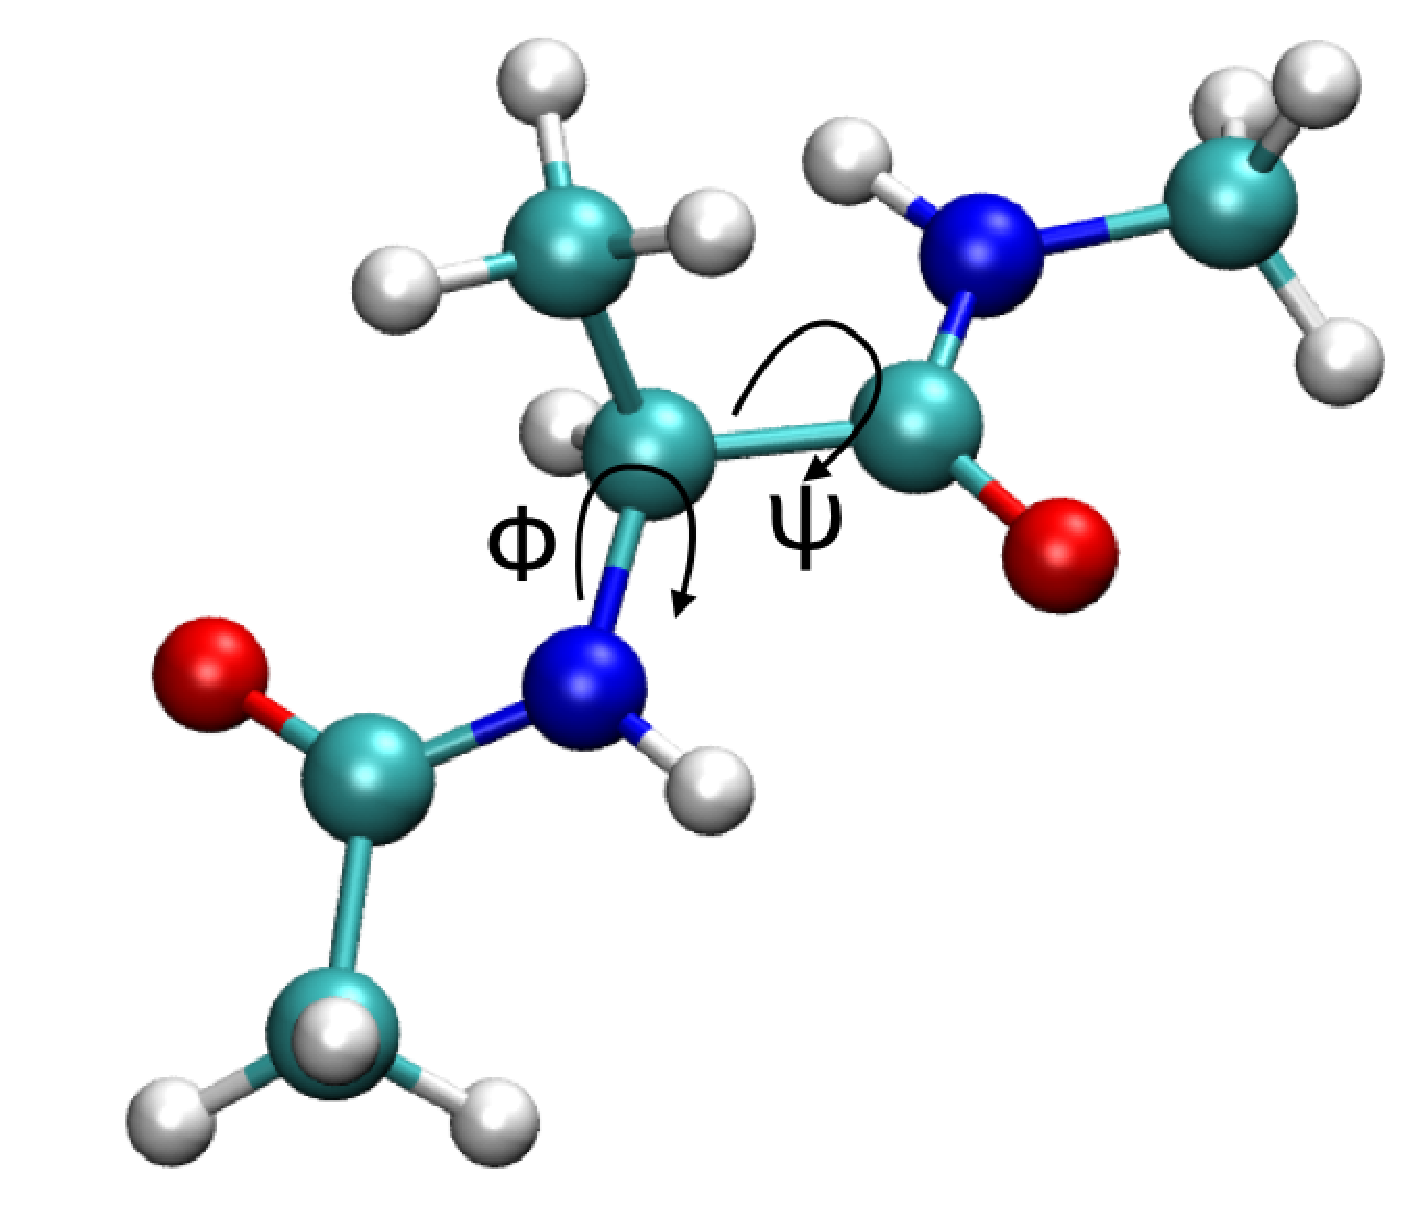
\includegraphics[width=10cm,angle=0]{./path/diala}
\caption{A sketch of the molecular structure of alanine dipeptide. The dihedral angles $\Phi$ and $\Psi$ are highlited.}
\label{diala}
\end{center}
\end{figure}
In this run we will perform 100 ps of NVT MD and check the evolution of the collective variables with this simple input (open
the file {\tt plumed.dat})
\esempio{
A very simple \plumed\ input file for monitoring the two $\Phi$ and $\Psi$ dihedral angles.\
 \vspace{10pt} 
{\tt
\# printout frequency\\
PRINT W\_STRIDE 10 \\
\# specify phi and psi\\
TORSION LIST 5 7 9 15   \\
TORSION LIST 7 9 15 17 \\
ENDMETA\\
}
} 
Now edit the script {\tt  build\_and\_run.sh}. This is a script that performs all the needed action for doing a 
run: it sources the correct environments, it creates the binary topology (this step is only required in GROMACS) and performs
the calculations. The only thing that you should do is to adapt it to your path, execute it (just by typing {\tt ./build\_and\_run.sh}) and you'll get a bunch of interesting stuff.

First of all you will get a {\tt md.log} file that contains some printout from \plumed\ so you may check wether the input was correctly 
read:
\begin{verbatim}
::::::::::::::::: READING PLUMED INPUT :::::::::::::::::
|-PRINTING ON COLVAR FILE EVERY 100 STEPS
|-INITIAL TIME OFFSET IS 0.000000 TIME UNITS

1-TORSION: (1st SET: 1 ATOMS), 
       (2nd SET: 1 ATOMS), (3rd SET: 1 ATOMS) , (4th SET: 1 ATOMS); 
|- 1st SET MEMBERS:  5 
|- 2nd SET MEMBERS:  7 
|- 3rd SET MEMBERS:  9 
|- 4th SET MEMBERS:  15 


2-TORSION: (1st SET: 1 ATOMS), 
       (2nd SET: 1 ATOMS), (3rd SET: 1 ATOMS) , (4th SET: 1 ATOMS); 
|- 1st SET MEMBERS:  7 
|- 2nd SET MEMBERS:  9 
|- 3rd SET MEMBERS:  15 
|- 4th SET MEMBERS:  17 

|-ANALYSIS: YOU WILL ONLY MONITOR YOUR CVs DYNAMICS
\end{verbatim}
This tells you that everything is going fine. The index of atoms are parsed correctly and the printout is correctly understood.
Now what you get is a {\tt COLVAR} file that consists in the time evolution of the CVs.
Its format looks something like this: \\
\begin{verbatim}
#! FIELDS time cv1 cv2 vbias vwall vext 
     0.000     -2.655213716      2.760231131      0.000000000      ...   
     0.020     -2.676506406      2.845943731      0.000000000      ...   
     0.040     -2.646984155      2.749365464      0.000000000      ...  
     ...      
\end{verbatim}
In the first line there is a simple remainder to the elements that you have in each column.
Namely time first (in ps by default in GROMACS), then the value of the two CVs followed by the 
various additional potential energies introduced by plumed. In this case there is no additional potential 
introduced and therefore all those columns are zeros.
Now you can plot the evolution of the CVs with gnuplot by using the  command
 {\tt  p "./COLVAR" u 1:2 t "Phi" ,"" u 1:3 t "Psi"}
 and you'll get something like Fig. \ref{plot_time}
\begin{figure}
\begin{center}
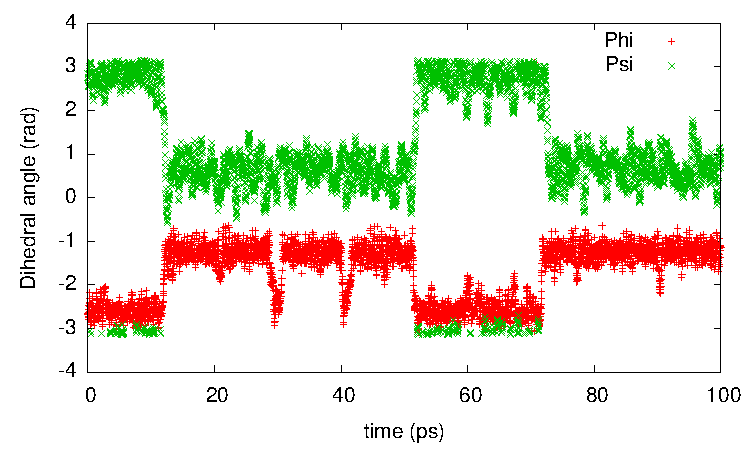
\includegraphics[width=12cm,angle=0]{./basics/monitoring/plot_time}
\caption{The time evolution of the variables $\Phi$ and $\Psi$}
\label{plot_time}
\end{center}
\end{figure}
If you want to  understand how they are related on the Ramachandran plot then you might use the command
{\tt p "./COLVAR" u 2:3} with gnuplot that results in a plot like that in Fig. \ref{plot_phipsi}.
\begin{figure}
\begin{center}
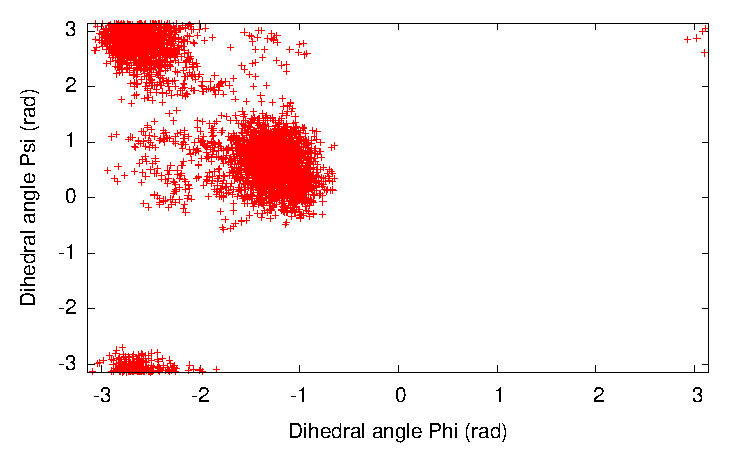
\includegraphics[width=12cm,angle=0]{./basics/monitoring/plot_phipsi}
\caption{The time population of the variables $\Phi$ and $\Psi$ during 100 ps run.}
\label{plot_phipsi}
\end{center}
\end{figure}

\section{Postprocessing with {\tt driver}}
\begin{verbatim}
#!/bin/bash
source  /usr/local/Modules/3.2.6/init/bash
module load intel-cc/10.1.015  
module load intel-fc/10.1.015 
module load fftw/3.2.2_intel-10.1.015
module load openmpi/1.2.6_intel-10.1.015
source /nfs_home/tutoadmin/PLUMED/EXERCISES
            /installation/gromacs/gromacs-4.0.7/install_dir/bin/GMXRC 
CATDCD="/nfs_home/tutoadmin/PLUMED/catdcd/LINUXAMD64/bin/catdcd4.0/catdcd"
TRJCONV="trjconv_d"
DRIVER="/scratch/tutoxx/1_compiling/plumed/PLUMED-1.2.1/utilities/driver/driver" 
mv COLVAR COLVAR.bak
#
# generate the pdb
#
echo 0 | $TRJCONV -f 2ala.gro -o 2ala.pdb
#
# generate the dcd 
#
$CATDCD  -o traj.dcd -trr traj.trr 
#
# run the driver
#
$DRIVER -pdb 2ala.pdb -dcd traj.dcd -ncv 2 -nopbc -plumed plumed2.dat 
\end{verbatim}
"Oh my god! I forgot to include that special CV!". No problem!
Max Bonomi wrote the {\tt driver} utility (you may find it in {\tt \$plumedir/utilities/driver })
through which you may postprocess your run and calculate that special CV you forgot to include 
runtime. Of course, being limited to the points for which you actually have the trajectory  you don't have much statistics unless
you collect very often the trajectory points (absolutely not recommended unless you want your supervisor hating you).
First compile it. Go into your \plumed\ directory ( should be someting like  {\tt /scratch/tutoxx/1\_compiling/plumed}). 
\begin{verbatim} 
cd PLUMED-1.2.1/
cd utilities/
cd driver/
ln -s ../../common_files/* .
module load intel-cc/10.1.015
module load  intel-fc/10.1.015
make intel
\end{verbatim}
Then you should convert the {\tt 2ala.gro} and {\tt traj.trr} into a pdb/dcd couple.
This can be done with trajconv (from GROMACS) and catdcd (from Klaus Schulten  group http://www.ks.uiuc.edu/Development/MDTools/catdcd/ )
At this stage you have what you need (a {\tt *.pdb} and {\tt *.dcd} couple).
This is done automatically by sourcing the correct executable from the script {\tt postprocess\_with\_driver.sh} (have a look into that, if you want to do this exercise automatically you should put the correct path). 
Let us assume that what you forget to calculate is now the distance for NME3:H (atom 18) - ACE1:O (atom 6) 
and ALA2:O (atom 16) - ALA2:H (atom 8) .
Then a you have to produce a new plumed input (say {\tt plumed2.dat} as in the example ) 
\esempio{
{\tt
\#\\ 
\# one printout each frame\\ 
\#\\ 
PRINT W\_STRIDE 1 \\
\#\\ 
\# the two distances for hydrogen bonds \\ 
\#\\ 
DISTANCE LIST 18 6  \\
DISTANCE LIST 16 8  \\
ENDMETA
}
}
and by using the following command (assuming that {\tt driver} points to the correct utility)
\begin{verbatim}
driver -pdb 2ala.pdb -dcd traj.dcd -ncv 2 -nopbc -plumed plumed2.dat 
\end{verbatim}
you get a new {\tt COLVAR} file with the data you need and by now you should be able to check the data you are obtaining with gnuplot.
All the previos commands are included {\tt postprocess\_with\_driver.sh}. By simply adapting it to your path and executing it you will have this exercise done.  

\chapter{Basics: biasing simulations}

\section{Restrained/steered molecular dynamics}

Once you define a bunch of collective variables of your interests \plumed\ has a number of ways in which you 
may affect their behavior. The fact that you can actually influence their value depends on the fact that each 
of the collective variables implemented in \plumed\ has analytical derivatives and, by biasing the value of a single CV 
one turns to affect the time evolution of the system itself.
The simplest way in which one might influence a CV is by forcing the system to stay close to a chosen value during the simulation.
This is achieved with umbrella potential that plumed provides via the  directive \keyword{UMBRELLA}

Very often it may happen that one wants that a given CV just stay within a given range of values. This is achieved in plumed 
through the directives \keyword{UWALL} and \keyword{LWALL} that act on specific collective variables and limit the exploration within given ranges.

Another useful strategy is the \keyword{STEERPLAN} directive. It allows to perform a series of programmed steered runs and can be helpful in
performing adaptive umbrella sampling or multievent reaction within a single simulation.
 
\subsection{An umbrella sampling calculation. Alanine dipeptide.}
As first example we perform an umbrella sampling calculation of the free energy landscape of alanine dipeptide with GROMOS96 all atom force field already seen in the previous section. In Fig. \ref{diala} you can see the 
molecular structure. Its free energy landscape is conveniently depicted as function of the two dihedral angles $\Phi$ and $\Psi$ (also called "Ramachandan plot"). An useful approach to depict the free energy landscape of this molecule is based on the so called "Umbrella Sampling" (US) algorithm. Without going much into details the calculation follows like this.
\begin{itemize}
\item Put an umbrella potential on a specified value of $\Phi$ and $\Psi$ (say $\Phi_0$ and $\Psi_0$).
\item Run a simulation and acquire reasonable statistics of the deviation of $\Phi$ and $\Psi$ respect to the position $\Phi_0$ and $\Psi_0$.
\item Change a bit the position of the restrain center $\Phi_0$ and $\Psi_0$ and start over a new simulation from the previous endpoint.
\item Iterate.
\end{itemize}  
By moving the restraint in with a "snake-like" evolution one can cover the whole range of values within the whole domain of interest $-\pi<\Phi<\pi$ and 
$-\pi<\Psi<\pi$ and, if the "clouds" of probability of restraints are overlapping, one can retrieve the Potential of Mean Force (PMF) by using the Weighted Histogram Analysis Method (WHAM). The program for WHAM is well established and can be downloaded from Alan Grossfield website (http://membrane.urmc.rochester.edu/content/wham).

The input for a single umbrella for \plumed\ is something like this:
\esempio{ A typical setup for a single umbrella in the umbrella sampling run

\vspace{10pt} 
{\tt
\#\\
\# only some printout for acquiring the statistics \\
\#\\
PRINT W\_STRIDE 10 \\
\#\\
\# set up two variables for Phi and Psi dihedral angles\\
\#\\
TORSION LIST 5 7 9 15   \\
TORSION LIST 7 9 15 17 \\
\#\\
\# Impose an umbrella potential on CV 1 and CV 2 \\
\# with a spring constant of 500 kjoule/mol \\
\# at fixed points on the Ramachandran plot\\
\#\\
UMBRELLA CV 1 KAPPA 500 AT     3.141593 \\
UMBRELLA CV 2 KAPPA 500 AT    -3.141593 \\
ENDMETA \\
}}
The syntax for the directive \keyword{UMBRELLA} is rather trivial. The directive is followed by a keyword \keyword{CV} followed by an index that
specify the number of the CV on which the umbrella potential has to act. The keyword \keyword{KAPPA} determines the hardness of the spring constant and its units are 
\begin{equation}
[Energy\ units\ of\ the\ program]/[Units\ of\ the\ CV]^2
\end{equation}
The additional potential introduced by the \keyword{UMBRELLA} takes the form of a simple Hooke's law:
\begin{eqnarray}
U(x)=\frac{\tt KAPPA}{2}(CV(x)-CV_0)^2
\end{eqnarray}
where $CV_0$ is the value specified following the \keyword{AT} keyword.
In output the sum of the additional potential is shown in the {\tt COLVAR} file. For this specific input the  {\tt COLVAR} file 
has in first column the time, in the second the value of CV 1, in the third the value of CV 2, in the fourth the potential from metadynamics (zero if 
metadynamics is not active), and in the fifth the additional potential introduced by umbrellas and walls. The position of the restrain is also reported
with the keyword \keyword{RST} followed by the index of the CV on which the umbrella potential is applied and the position of the constraint.  

The procedure explained before is summarized by the script {\tt script.sh} that you find in the exercise folder.
%\begin{verbatim}
%#!/bin/bash
%GROMPP="/PATH_TO_GROMACS/grompp"
%MDRUN="/PATH_TO_GROMACS/mdrun"
%nstep=25
%incr=0
%ks=500
%pi=3.14159265358979
%start_config="2ala.gro"
%input_file="md.mdp"
%topol="gromacs.top"
%indexfile="index.ndx"
%#####################################################
%# here starts the umbrella sampling run 
%#####################################################
%rm -rf metadatafile CV_*
%for i in  `seq 0 $nstep`
%    do
%    val1=`echo $i\*2\* $pi/$nstep - $pi   | bc -l | awk '{printf("%12.6f",$1)}'`
%    for j in  `seq 0 $nstep`
%        do
%        # 0 go forth 1 go back
%        dir=`echo ${i}%2 | bc `
%        if  [ "$dir" -eq "0" ]; then
%        val2=`echo $j\*2\* $pi /$nstep - $pi | bc -l | awk '{printf("%12.6f",$1)}' `
%        else 
%        val2=`echo $pi -$j\*2\* $pi /$nstep  | bc -l | awk '{printf("%12.6f",$1)}'`
%        fi
%        incr=$((incr + 1)) 
%        #
%        # at the very beginning do first a steering 
%        # where you intend to start the dynamics
%        #
%        if [ "$incr" -eq "1" ]; then
%          cat >metadyn.dat <<EOF
%          PRINT W_STRIDE 10 
%          TORSION LIST 5 7 9 15   
%          TORSION LIST 7 9 15 17 
%          UMBRELLA CV 1 KAPPA ${ks} AT ${val1}
%          UMBRELLA CV 2 KAPPA ${ks} AT ${val2}
%          ENDMETA
%EOF
%          #
%          # preprocess with grompp
%          #
%          $GROMPP -f md.mdp -c 2ala.gro -p gromacs.top -n index.ndx &>/dev/null 
%          $MDRUN -plumed metadyn &>/dev/null
%        fi
%        echo "ANG1 $val1 ANG2 $val2 INCR $incr"
%        cat >metadyn.dat <<EOF
%        PRINT W_STRIDE 10 
%        TORSION LIST 5 7 9 15   
%        TORSION LIST 7 9 15 17 
%        UMBRELLA CV 1 KAPPA ${ks} AT ${val1}
%        UMBRELLA CV 2 KAPPA ${ks} AT ${val2}
%        ENDMETA
%EOF
%        #preprocess and run
%        $GROMPP -f md.mdp -c confout.gro -p gromacs.top -n index.ndx &>/dev/null 
%        $MDRUN -plumed metadyn &>/dev/null
%        grep -v FIELDS COLVAR | awk '{printf("%12.6f %12.6f %12.6f\n",$1,$2,$3)}'  >CV_${incr}
%        echo "CV_${incr} ${val1} ${val2} ${ks} ${ks} ">>metadatafile 
%        rm -rf \#*
%        done
%done
%\end{verbatim}
After you run that script you should end up with a file called {\tt metadatafile} and a number of files having names like {\tt CV\_*}.
The file {\tt CV\_*} contain the time and the value of the CVs at each time. These are produced by the script itself by simple
postprocessing of the {\tt COLVAR} file. The {\tt metadatafile} contains the name of each time evolution
{\tt CV\_*} followed by the center of the springs and the spring constants.  
The {\tt wham-2d } program just need the {\tt metadatafile} and {\tt CV\_*}.
The simple command 
\begin{verbatim}
wham-2d Px=pi -3.14159 3.14159 50 Py=pi -3.14159 3.14159 
            50 0.001 300 0 metadatafile free_ene.dat >out_wham  
\end{verbatim}
should be sufficient in producing the free energy landscape in 2d that is represented in \ref{ramagromos}.
In the end you should get something like that in Fig. \ref{ramagromos}. 
\begin{figure}
\begin{center}
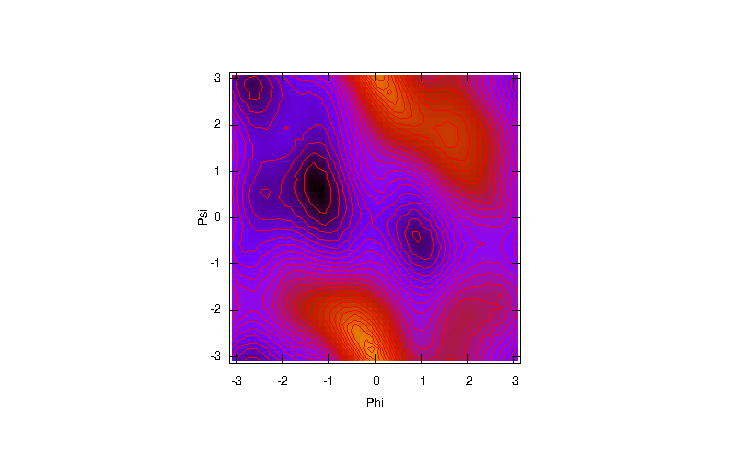
\includegraphics[width=15cm,angle=0]{./path/umbrella_sampling/rama_gromos96}
\caption{The free energy landscape of an alanine dipeptide with the GROMOS96 all\-atom force field. Isolines are drawn every 1kcal/mol.}
\label{ramagromos}
\end{center}
\end{figure}
You might obtain such a plot by using this simple gnuplot script:
\begin{verbatim}
set term pdf noenhanced 
set out "rama_gromos96.pdf"
unset key
unset colorbox
set size square
set multiplot
set view map
set xr [-pi:pi] 
set yr [-pi:pi] 
spl "free_ene.dat" u  1:2:3 w pm3d
set xlab "\Phi"
set ylab "\Psi" 
unset surf
set contour base
set cntrp lev incr 0,1,40
unset pm3d
unset clabel
spl "free_ene.dat" u 1:2:3 w l 
quit
\end{verbatim}


\subsection{A steered molecular dynamics example: targeted MD.}
As a second example of the restraint features of \plumed\ we discuss here the use of the directive \keyword{STEER}.
Very often it is useful to drag the system from an initial configuration to a final one by pulling one or more CVs.
Most of time the aim of such simulations is to prepare the system in a particular state or produce nice snapshots for a cool movie. 
The reason behin the limited usefulness of such simulations is that in most of the cases these are "out-of-equilibrium" simulations and they are 
not representative of equilibrium ensemble that is generally of interest for simulations.
However, Jarzynski \cite{jarzynski} inequality provides a connection between out-of-equilibrium trajectories and equilibrium free energy differences. 
This inequality consists in:
\begin{equation}
\Delta F = -\beta^{-1} \ln<\exp (-\beta W)>
\end{equation}
where the average is calculated over the work obtained from a number of out-of.equilibrium trajectories. $\beta$ is $k_bT$ and $\Delta F$ is the free energy difference.  The value of $W$ can be obtained via 
\begin{eqnarray}
W=\int_0^{t_s}dt\ \frac{\partial H_\lambda(t)}{\partial t}
\end{eqnarray}
where $H_\lambda$ is a modified hamiltonian which contains an additional term, namely:
\begin{eqnarray}
H_\lambda(t)&=&H+U_\lambda(t)\\
&=&H+\frac{k}{2}(CV(x)-\lambda(t))^2\\
&=&H+\frac{k}{2}(CV(x)-CV_0-vt)^2.
\end{eqnarray}
From which it comes naturally that the derivative is simply:
\begin{eqnarray}
\frac{\partial H_\lambda(t)}{\partial t}&=&-vk(CV(x)-CV_0-vt)\\&=&-vk(CV(x)-\lambda(t))
\end{eqnarray}
and therefore the integral $W$ can be obtained simply by quadrature summing up all the deviation respect to 
the position of the mobile center of the harmonic restraint.

In the limit of lots of pulling therefore meaningful free energy differences can be retrived.
Here in this example we do not focus on the Jarzynski limit but on the details on how to steer a molecule fo alanine dipeptide towards one of
its minima. We first prepare the system around $\Phi\simeq-2.6, \Psi\simeq2.8$  (see Fig. \ref{ramagromos}) and we pull the heavy atoms towards
the other minimum located around $\Phi\simeq1, \Psi\simeq-0.5$. In order to do that we won't use the two dihedrals but an input pdb representing
the heavy atoms in that situation. This is generally called "Targeted MD".
The input looks like:
\esempio{
{\tt
PRINT W\_STRIDE 100 \\
\#\\
\# create a cv that measure MSD from a reference structure\\
\#\\
TARGETED TYPE RMSD FRAMESET min.pdb\\
\#\\
\# steer this CV to a value of 0.0 \\
\#\\
STEER CV 1 TO 0.0 KAPPA 10000000.0 VEL 0.0001 \\
\#\\
\# additional variables that may be useful \\
\#\\
TORSION LIST 5 7 9 15   \\
TORSION LIST 7 9 15 17 \\
ENDMETA\\
}
}
Note the syntax of the \keyword{TARGETED} that is intended to use a reference in MSD space (min.pdb in this case).
The syntax of \keyword{STEER} is also specified. It requires a keyword \keyword{CV} in order to specify the index of the variable on which 
the steering has to be carried out. In this system there are three variables (TORSION are also CVs) but only the first CV (TARGETED) has to be steered to a given value. The target value is specified by the keyword \keyword{TO} followed by the value that has to be reached.
Then the keyword \keyword{KAPPA} comes and specify the hardness of the spring constant (in this case the units are $\rm (kjoule/mol)/nm^4$ as the units of the \keyword{TARGETED} variable are $\rm nm^2$. This is true only for GROMACS. Other programs adopt $\rm \AA^2$).
One can follow the evolution  through gnuplot by visualizing the instantaneous value of the CV and the position of the moving constraint
by the simple command {\tt p "./COLVAR" u 1:2 t "CV","" u 1:10 t "Moving constraint"} and obtain a plot like the one reported in Fig. \ref{followsteered}.
\begin{figure}
\begin{center}
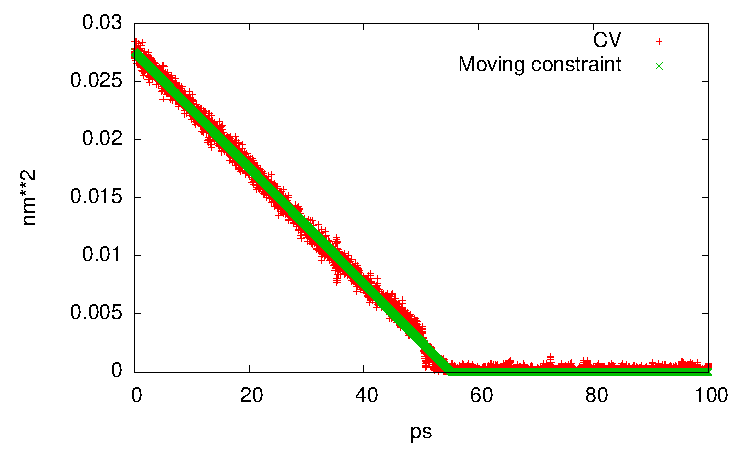
\includegraphics[width=10cm,angle=0]{./biasing/steered/figure}
\caption{Following a steered MD run during time}
\label{followsteered}
\end{center}
\end{figure}
Now we can also give a try in calculating the work $W$. 
Run the awk script with the command:\\
{\tt ./integrate.awk time=1 cv=2 constr=10 kappa=10000000.0 COLVAR  >work.dat}�\\
and plot work.dat with gnuplot and the command {\tt p "./work.dat" u 2:(\$3/4.186) w lp}
so you will obtain a plot of the work (see Fig. \ref{worksteered}).
\begin{figure}
\begin{center}
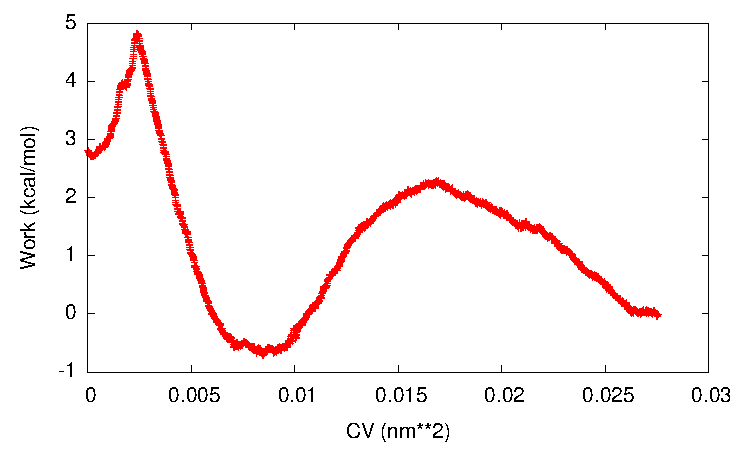
\includegraphics[width=10cm,angle=0]{./biasing/steered/work}
\caption{The  work calculated during a steered MD run.}
\label{worksteered}
\end{center}
\end{figure}

\subsection{A programmed steered MD with steerplan.}
Another feature that is implemented in \plumed\ is a "tunable" moving restraint called \keyword{STEERPLAN}.
The basic idea behind is the fact that many times what one wants to study is a multistep process. For example
consider an enzymatic reaction which is made of several proton transfers and nucleophilic attack. 
It can be rather usefil whenever one needs to create a guess path  for path collective variables calculations. Instead of creating
multiple steered MD run, each of those has a single cv which is steered at a time, you can put all the variables in a single 
\plumed\ input and then plan the steering so that you first steer one CV then you switch this potential off and switch another potential
that steers a different CV, all within a single run. In this example we will see the usual alanine dipeptide and we will reach the minimum at   $\Phi\simeq1, \Psi\simeq-0.5$ through a two-step process. First we will pull $\Psi$ to  -0.5 and keep $\Phi$ fixed at -2.6, then we will pull $\Phi$ to 1.0 and then release all the constraint.
The input is simple
\esempio{
{\tt
PRINT W\_STRIDE 100\\ 
\#\\
\# Phi and psi angles\\
\#\\
TORSION LIST 5 7 9 15 \\  
TORSION LIST 7 9 15 17 \\
\#\\ 
\# steerplan\\
\#\\
STEERPLAN myplan\\
ENDMETA
}
}
The keyword \keyword{STEERPLAN} expects a file whose name is {\tt myplan} in this case that contains the rules for the programmed steering.
In this case it looks like this:
\begin{verbatim}
 0.000  CV 1  100.0 -2.6   CV 2     100.0  2.8 
30.000  CV 1  100.0 -2.6   CV 2     100.0 -0.5 
60.000  CV 1  100.0  1.0   CV 2     100.0 -0.5 
70.000  CV 1    0.0  1.0   CV 2       0.0 -0.5 
\end{verbatim}
which means: at time 0.0 put an harmonic constraint on the CV 1 whose hardness is 100 kjoule/mol centered on the value -2.6. On the CV 2 do the same but centered on the 
value 2.8. At later time (30 ps) the constraint on CV 1 is the same while on CV 2 its center should be now at 0.5. Thus the program is keeping a fixed harmonic constraint on the 
first variable while moving the second up to reaching -0.5. From 30 ps to 60 ps is the CV 1 that should move from -2.6 to 1.0. Finally, from 60 to 70 ps the springs are switched off 
(the spring constant are put to 0.0) and the system is now free to thermalize in the new minimum. Consider that \keyword{STEERPLAN} allows the use of wildcards {\tt *} on the 
position of the constraint whose meaning is "start with an umbrella centered where the system is" (please see the manual for the full documentation).
{\tt COLVAR} file reports in the final columns the steerplan action in progress denoted by {\tt STP} which is followed by something like :
\begin{verbatim}
 CV  1 X    -2.600000 K   100.000000 T 1 
\end{verbatim}
that tells on which CV  the steerplan is active, where is the center of the potential, the spring constant and the type of the potential used (there exist three different types {\tt CENTRAL} whose code is 1,  {\tt POSITIVE} whose code is 2, {\tt NEGATIVE} whose code is 3. See manual for further details).
After you run the example it is straightforward to understand what happened by plotting the {\tt COLVAR} file with gnuplot by using the following command: 
{\tt p "./COLVAR" u 2:3 t "CVs","" u 13:21 t "designed path"}
(see Fig. \ref{steerplan}) .
\begin{figure}
\begin{center}
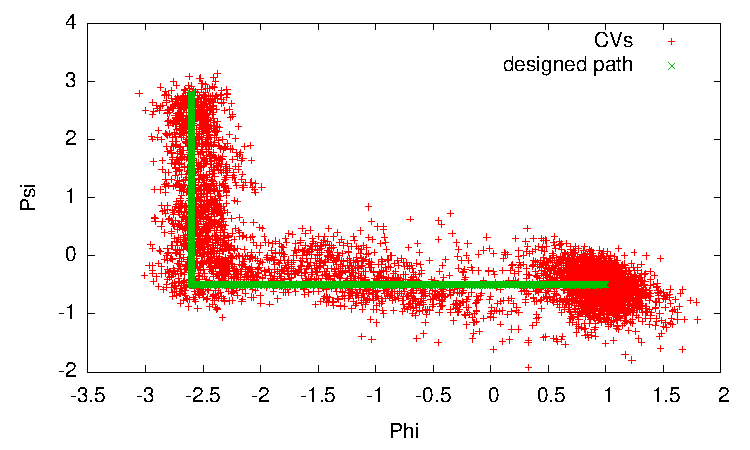
\includegraphics[width=10cm,angle=0]{./biasing/steerplan/figure}
\caption{Evolution of the CV when steerplan is used.}
\label{steerplan}
\end{center}
\end{figure}

\subsection{Soft walls}\label{softwall}
\plumed\ implements soft and hard walls. Here the soft walls are explained.
Very often during a metadynamics simulation it might happen that one wants to avoid to sample some regions because they are not
chemically relevant for the pricess under study.  In this case one can adopt the so-called "walls". In \plumed\ there exist two kind of walls:
\keyword{LWALL} (lower wall) and  \keyword{UWALL} (upper wall). They act on two different directions. 
\keyword{LWALL} prevents the system to go lower than a specified value while \keyword{UWALL} prevents the system to explore regions whose CV is higher than a specified value. This is achieved by using (by default) a fourth order harmonic function. Some parameters can also be tuned.
The walls take the form for values larger or smaller than {\tt LIMIT} in case of \keyword{UWALL}  and \keyword{LWALL} respectively:
\begin{equation}
V_{wall}(s)=\mathtt{KAPPA}  \left (\frac{s- \mathtt{LIMIT}+ \mathtt{OFF}}{\mathtt{EPS}} \right)^{\mathtt{EXP}}, 
\end{equation}
where {\verb KAPPA } is an energy constant in internal unit of the code,
{\verb EPS } a rescaling factor and {\verb EXP } the exponent determining the power law. 
By default: $\mathtt{EXP}=4, \; \mathtt{EPS}=1.0, \; \mathtt{OFF}=0$ and are optional arguments
In the exercise we run alanine dipeptide in a region close to the saddle point.
In order to do that we confine with \keyword{UWALL}  and \keyword{LWALL}  the variable $\Phi$.
The \plumed\ input looks something like this
\esempio{
{\tt
PRINT W\_STRIDE 100 
\#\\
\# Phi and psi angles\\
\#\\
TORSION LIST 5 7 9 15   \\
TORSION LIST 7 9 15 17 \\
\#\\
\# LWALL: a lower wall  \\
\# UWALL : an upper wall \\
\#\\
UWALL CV 1 LIMIT  0.1 KAPPA 100.0 EXP 4.0 EPS 1.0 \\
LWALL CV 1 LIMIT -0.1 KAPPA 100.0 EXP 4.0 EPS 1.0\\
ENDMETA
}
}
The syntax for \keyword{LWALL} and  \keyword{UWALL} closely resembles
the ones from the \keyword{UMBRELLA}. You can at this point easily figure out its meaning.
\keyword{LIMIT} needs to be followed by one number that specifies the bundary. 
\keyword{KAPPA} is the spring constant. 
Have a look to the CVs during the run by using the command in gnuplot: 
 {\tt p "./COLVAR" u 2:3}. You can notice that the variable very often passes the imposed boudaries. 
 This is not surprising because the spring potential simply discourage to sample those regions but is does
 not a-priori forbids their exploration. By tuning \keyword{KAPPA} one can limit the exploration to the imposed region.
 Try harder \keyword{KAPPA}s. What does it happen?
 
\section{Committment analysis}

At this stage it might be interesting to figure out you may use \plumed\ and GROMACS together in a single bash 
script so to perform useful tasks. One of this task is the calculation of the so-called "committor" function.
A central issue of the rare events research is how to judge wether a given transition state (i.e. a saddle point) in the free energy 
has the expected dynamical meaning. Without dwelling into details (see the good literature for that \cite{Bolhuis:2000p8198,Maragliano:2006p6867,Ren:2005p5706,Peters:2010p15801,Peters:2006p660,Peters:2006p411}) the committor probability is calculated
as the probability of falling into product state before falling into the reactant state when starting from a given point in the phase space (that can be a given region in the collective variable). Therefore, we added this section here as in the previous exercise we already collected a bunch 
of point along the transition state. This is evident if you plot the Ramachandran angles in the usual way. You might find that part of the points
fall at $\Phi<0$ and part fall at $\Phi>0$ that suggest that, across the point $\Phi\simeq 0$ you have a transition state of some kind.
Further proof of it can be obtained from Fig. \ref{ramagromos}.
In order to do this we first collect some points along the TS with the run having walls (see Sect. \ref{softwall} ) because previously no
frames were collected in the trajectory (you can tune this in GROMACS input with the flag {\tt nstxout}).
Then we have to follow this workflow:
\begin{itemize}
\item Convert {\tt traj.trr} into a dcd (using {\tt catdcd}).
\item Convert {\tt 2ala\_ts.gro} into a pdb (using {\tt trjconv}).
\item Postprocess the {\tt \*.pdb} and {\tt \*.dcd} with the {\tt driver} so to retrieve the exact position of $\Phi$ per each frame
\item Postprocess the {\tt COLVAR} file produced by the  {\tt driver} through {\tt awk} and create a series of files containing the indexes of the frames along the trajectory for each slice along the collective variable.
\item For each frame contained in each slice, run a MD with the \plumed\ file containing the {\tt STOPWHEN} keyword so to kill the run as soon as it reaches one boundary. In this case we consider to kill the run when $\Phi<-0.8$ or $\Phi>0.8$ and we increase a counter only if the 
reactant is reached.
\item At the end of running all the frames contained in the slice, then the ratio between the frames that reached the reactant and the total number of frames give the resulting value of the committor.
%\item
%\item
%\item
%\item
\end{itemize}
Have a look to the script {\tt committor.sh}: it contains all the steps to perform this simple committor analysis. 
If you launch it with {\tt ./committor.sh >outcomm }
at the end you should obtain a plot like the one in Fig. \ref{committor}.
\begin{figure}
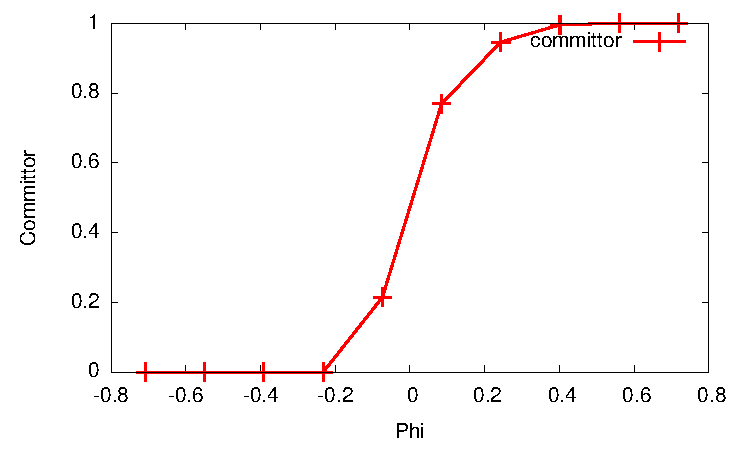
\includegraphics[]{biasing/committor/committor}
\caption{The committor as calculated in the exercise.}
\label{committor}
\end{figure}

\section{Metadynamics}

Metadynamics adds an external potential to the simulation.
This bias potential acts on a restricted number of degrees of
freedom of the system $\bm{S}(\bm{R})=(S_1	(\bm{R}),...,S_d(\bm{R}))$ often referred to as collective variables or CVs.
The metadynamics potential $V(\bm{S},t)$ varies with time $t$ and is constructed 
as a sum of Gaussian functions, or hills, deposited during the simulation:

\begin{equation}
V(\bm{S},t)=\int_0^t\ dt^\prime \omega\exp\left(-\sum_{i=1}^{d} 
\frac{(S_i(\bm{R})-S_i(\bm{R}(t^\prime))^2}{2\sigma_i^2} \right),
\end{equation}

where $\sigma_i$ is the Gaussian width corresponding to the $i$-th CV
and $\omega$ the rate at which the bias grows.
In the practice, Gaussians of height equal to $W$ are deposited every $\tau$ MD steps,
so that $\omega=W / \tau$.

In order to perform a metadynamics simulation we have to:
\begin{itemize}
\item Choose wisely the set of CVs to address the problem. This is a long story. 
To cut it short, CVs 
a)  should clearly distinguish between the initial state, the final state and the intermediates,
 b) should describe all the slow events that are relevant to the process of interest,
c) their number should not be too large, otherwise it will take a very long time to fill the free energy surface.

\item Choose the Gaussian height $W$ and the deposition stride $\tau$.
These two variables determine the rate of energy added to your simulation. 
If this is too large, the free energy surface will be explored at a fast pace, 
but the reconstructed profile will be affected by large errors. 
If the rate is small, the reconstruction will be accurate, but it will take a longer time.
The error on the reconstructed FES depends on the ratio $W/\tau$, not on the two parameters alone \cite{error}.
\item Choose the Gaussian width $\sigma_i$. This parameter determines the resolution
of the reconstructed FES. The sum of Gaussians reproduces efficiently 
(\emph{i.e.} in a finite simulation time) features of the FES on a scale larger than $\sigma_i$. 
A practical rule is to choose the width as a fraction (half or one third) of the
CV fluctuations in an unbiased simulation. This is not a golden rule, since the value of the fluctuations
is not universal but usually depends on the position in the CV space. 
\end{itemize}

To activate a metadynamics calculation in \plumed \ you have to use the
directive {\tt HILLS}. The deposition stride $\tau$ is specified in unit of
time steps by the keyword {\tt W\_STRIDE}, the height $W$ by {\tt HEIGHT} in 
internal units of energy of the MD code used. The Gaussian width $\sigma_i$ must
be specified on the line of each CVs with the keyword {\tt SIGMA}.  

A typical \plumed \ input file for a metadynamics calculation looks as follows. 

\esempio{{\tt
HILLS W\_STRIDE 1000 HEIGHT 0.4 \\
TORSION LIST 5 7 9 15 SIGMA 0.35 \\
ENDMETA
}}

Beside the usual {\tt COLVAR} file, when you run a metadynamics calculation you
get an additional file called {\tt HILLS} which contains a list of the Gaussians
deposited during the simulation. 
In the example above, this file would look like: 

\begin{verbatim}
     1.000     -2.617548716      0.350000000      0.400000000   0.000 
     2.000     -2.718742869      0.350000000      0.400000000   0.000 
     3.000     -2.662313657      0.350000000      0.400000000   0.000 
     4.000     -2.378730722      0.350000000      0.400000000   0.000 
     5.000     -2.120031391      0.350000000      0.400000000   0.000 
\end{verbatim}

where:

\begin{itemize}
\item the first column contains the time $t$ (in internal unit of the MD code) at which
the Gaussian was deposited;
\item the following $d$ columns contain the centroid of the Gaussian, $S_i(\bm{R}(t))$, one for each CV $i$;
\item the following $d$ columns contain the Gaussian sigma $\sigma_i$, one for each CV $i$;
\item the last but one column contains the value of $W$;
\item the last column is meaningful only in well-tempered metadynamics simulations (see below).
\end{itemize}

This file will be used to calculate the estimate of the free-energy at the end of our metadynamics calculation.

Beside the metadynamics CVs, we can add other variables that we want to monitor during the simulation.
A typical \plumed \ input file looks as follows.

\esempio{Here we want to run a metadynamics calculation using a dihedral as CV. 
During the run we want to monitor the evolution of another dihedral angle. \vspace{10pt} \\
{\tt 
PRINT W\_STRIDE 500 \\
HILLS W\_STRIDE 1000 HEIGHT 0.4 \\
TORSION LIST 5 7 9 15 SIGMA 0.35\\
TORSION LIST 7 9 15 17 \\
ENDMETA
}}

The evolution of the additional variable can be monitored by looking at the {\tt COLVAR} file.

\begin{verbatim}
#! FIELDS time cv1 cv2 vbias 
     0.000     -2.655726464      2.760989206      0.000000000 
     0.500     -2.492360677      1.370313209      0.000000000 
     1.000     -2.617548716     -0.807834974      0.400000000 
     1.500     -2.163294675      0.453630761      0.172299337 
     2.000     -2.718742869     -0.557066598      0.783627027  
     2.500     -2.743156519      0.246435084      0.774082974   
     3.000     -2.662313657      0.024026518      1.191579452
\end{verbatim}

\section{Restarting metadynamics}

In order to restart a metadynamics run, the flag {\tt RESTART} must be added on the line of the directive {\tt HILLS}.
This allows a metadynamics simulation to be restarted after
an interruption or after a run has finished. The {\tt HILLS} files will be read
at the beginning of the simulation and the bias potential applied to the
dynamics. Note that the presence of the {\tt RESTART} flag only affects
the metadynamics part of the simulation, and thus the usual procedure for
restarting a MD run must be followed. This depends on the
particular MD engine used and can be found in the relative documentation.
\esempio{The following is an example of input file for restarting a metadynamics simulation.  \vspace{10pt} \\
{\tt
HILLS RESTART W\_STRIDE 1000 HEIGHT 0.4 \\
TORSION LIST 5 7 9 15 SIGMA 0.35\\
ENDMETA
}}

\section{Free-energy reconstruction}\label{fes-reconstr}

In the long-time limit, the bias potential of metadynamics converges to the free-energy changed in sign \cite{bussi_noneq}.
At any time during the simulation we can sum the Gaussians deposited so far and obtain the current estimate
of the FES using the utility {\tt sum\_hills}.
This code is very flexible and can be executed with several options (see the manual).
The most commonly used are:

\esempio{{\tt
  sum\_hills -file HILLS -out fes.dat -ndim 3 -ndw 1 2 -kt 0.6 -ngrid 100 100 100 \vspace {10pt} \\
   \begin{tabular}{ l l }
   -file           & input file with the list of Gaussians\\
   -out            & output file with the FES\\
   -ndim           & number of collective variables \\
   -ndw            & ID of the variables for FES in output \\ 
   -ngrid          & grid mesh dimension\\
   -dp             & grid bin size\\
   -kt             & $kT$ in the energy units\\
   -stride         & how often the FES is written\\
   -2pi            & ID of the variables with $[0;2\pi]$ periodicity \\
   -pi             & ID of the variables with $[-\pi;\pi]$ periodicity \\
  \end{tabular}
}}

The file in output {\tt fes.dat} contains the estimate of the free-energy calculated
on a regular grid whose dimension is specified by either {\tt -ngrid} or {\tt -dp}. 
These parameters should be chosen with care. To calculate accurately the potential in a given point of the CV space, 
a practical rule is to choose the bin size to be half the Gaussian sigma.

The {\tt sum\_hills} code should be used to monitor the convergence of a metadynamics simulation. 
This can be easily achieved by calculating the estimate of the FES at regular interval in time
using the {\tt -stride} option and then evaluating the free-energy difference among 
relevant regions (minima) of the FES as a function of time.
Below we report an example of bash script that can be used for this purpose.

\esempio{Example of script to evaluate the convergence of a metadynamics run.
Here we performed a metadynamics calculation using 2 CVs. We have defined two
regions in the projection of the FES onto the first variable. The F region in which
CV1 is greater than 2, and the U region in which CV1 is lower than 2.
The free-energy difference between F and U is calculated as a function of time
and saved in the file {\tt DeltaF}. \vspace{0.5cm} \\
{\tt
\#!/bin/bash \\
 sum\_hills -stride 100 -ndim 2 -ndw 1 -ngrid 100 100 -kt 0.6 -file HILLS \\
 for file in fes.dat.? fes.dat.?? fes.dat.??? \\
 do \\
  if [ -f \${file} ]; then \\
    F=`awk 'BEGIN\{tot=0\}\{if(NF==2 \&\& \$1>2.0)tot=tot+exp(-\$2/0.6)\}END\{print -0.6*log(tot)\}' \$file` \\
    U=`awk 'BEGIN\{tot=0\}\{if(NF==2 \&\& \$1<=2.0)tot=tot+exp(-\$2/0.6)\}END\{print -0.6*log(tot)\}' \$file` \\
    delta=`echo "\$F - \$U" | bc -l` \\
    echo \$delta >> DeltaF \\
  fi 
}}


\begin{figure}[!h]
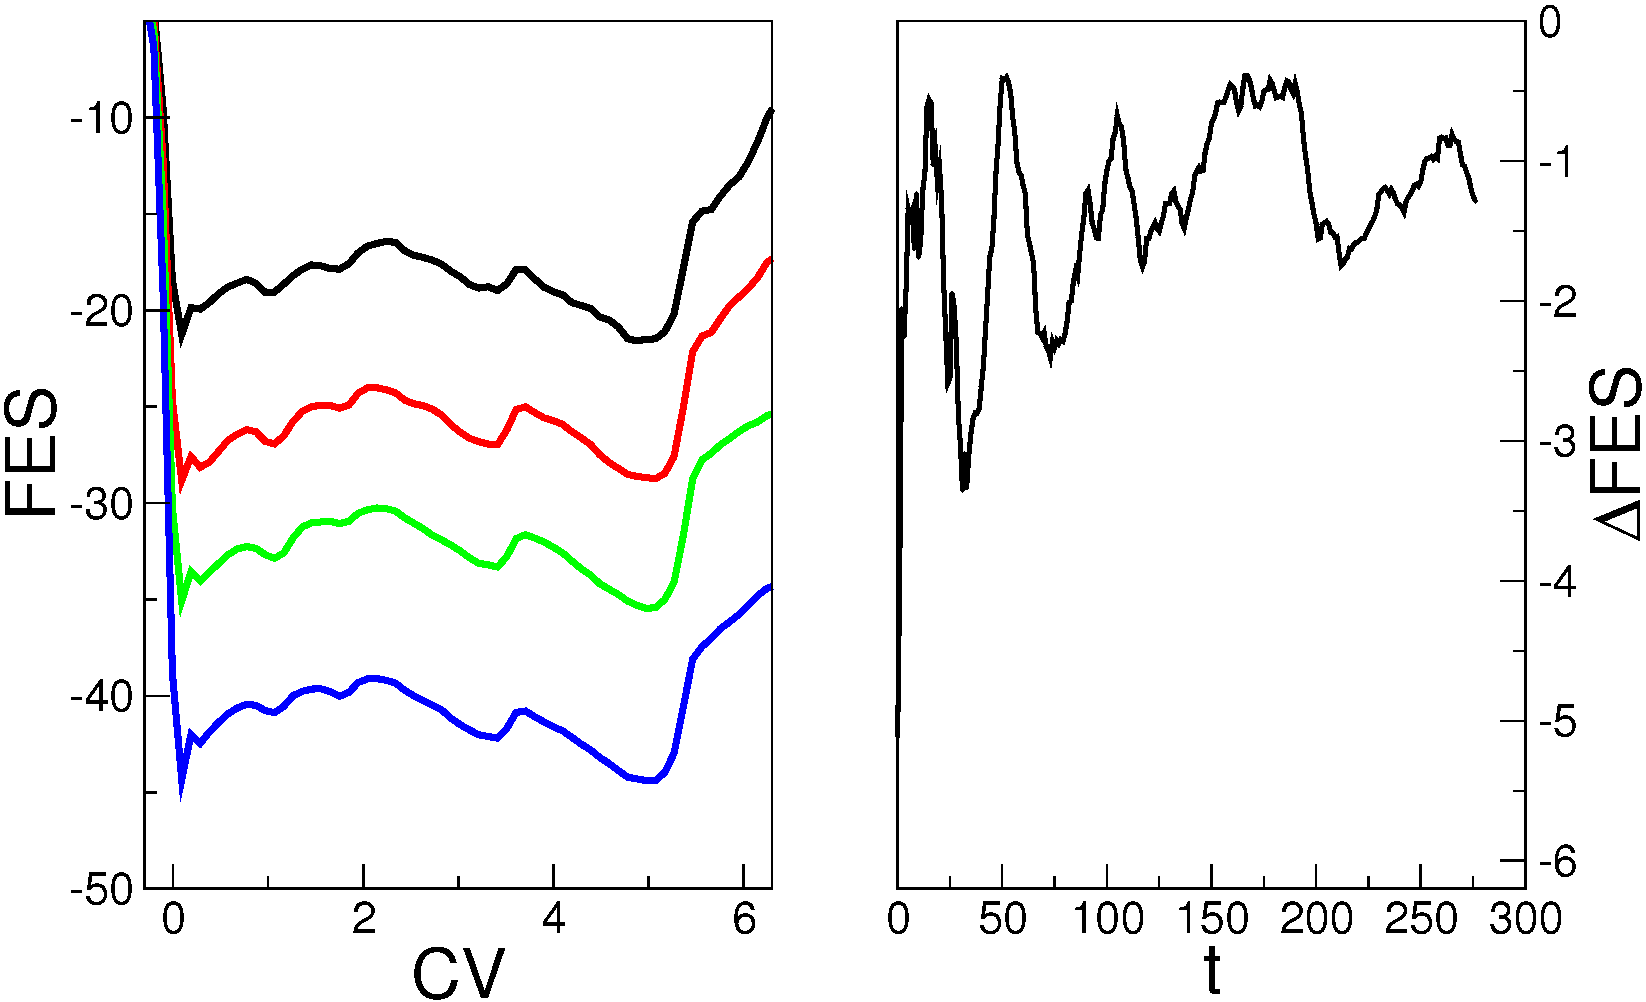
\includegraphics[width=1.0\linewidth]{figures/convergence}
\caption{Checking the convergence of a metadynamics run. Left panel. Free-energy estimate at different time steps. 
Right panel. Free-energy difference between state F and U as a function of time.}
\label{check_conv}
\end{figure}

\clearpage

\section{Well-tempered metadynamics}

In well-tempered (WT) metadynamics, the Gaussian height $W$ is automatically rescaled during the simulations
following:
\begin{equation}
W=W_0 \, e^{-\frac{V(\bm{S},t)}{k_B \Delta T}},
\label{WT}
\end{equation}
where $W_0$ is the initial Gaussian height and $\Delta T$ a parameter with the dimension of a temperature.
The use of Eq. \ref{WT} guarantees that the bias potential converges in a single simulation and does not
oscillate around the FES value, causing the problem of overfilling:
\begin{equation}
V(\bm{S},t \rightarrow \infty) = -\frac{\Delta T}{T + \Delta T} F(\bm{S}) +C, 
\end{equation}
where $T$ is the temperature of the system and $C$ a costant.

The quantity $T+\Delta T$ is often referred to as the (fictitous) CV temperature, while
the ratio $(T+\Delta T) / T$ as bias factor. 
To perform a WT metadynamics simulation with \plumed \ you have to 
use the directive {\tt WELLTEMPERED} and specify one of the parameters described above using
either the keyword {\tt CV\_TEMPERATURE} or {\tt BIASFACTOR}.
In addition, the temperature of the system must be specified explicitly with {\tt SIMTEMP}.

Here are some practical rules to choose wisely the parameters in WT metadynamics simulations:
\begin{itemize} 
\item The bias factor (or equivalently the CV temperature) regulates how fast the amount of bias 
potential added decreases with simulation time and eventually controls the extent of exploration.
The choice of these parameters depends on the typical free-energy barriers
involved in the process under study. 
In biomolecular simulation, a bias factor of 10-15 which
corresponds to barriers of the order of 6-9 kcal/mol at 300K is usually
appropriate. Note that this parameter can be changed on-the-fly as needed. 

\item The optimal choice of the initial Gaussian height $W_0$ is less crucial
and at the same time less trivial. It is irrilevant in the long time regime and affects only the transient part of the
simulation. A short initial filling period can be desirable if the transverse degrees of freedom
relax quickly, otherwise a moderate initial energy rate is a better choice. 
\end{itemize}


\esempio{The following is an example of input file 
for a WT metadynamics simulation at 300 (internal units of temperature) with a bias factor equal to 15 and an initial
Gaussian height of 0.4 (internal units of energy). \vspace{10pt} \\
{ \tt
HILLS W\_STRIDE 1000 HEIGHT 0.4 \\
WELLTEMPERED SIMTEMP 300 BIASFACTOR 15 \\
TORSION LIST 5 7 9 15 SIGMA 0.35 \\
ENDMETA 
}}

In WT metadynamics, the Gaussians height as written in the {\tt HILLS} file
is multiplied by the factor $(T+\Delta T)/ \Delta T$. This guarantees that
when you sum the Gaussians (by means for example of the {\tt sum\_hills} code) you get directly the FES.
The last column of the {\tt HILLS} file contains the value of the bias factor used in the
WT metadynamics simulation. For the example above, this file would look like:

\begin{verbatim}
     1.000     -2.617548716      0.350000000      0.428571429   15.000 
     2.000     -2.718742869      0.350000000      0.423889087   15.000 
     3.000     -2.662247736      0.350000000      0.419017741   15.000 
     4.000     -2.380845469      0.350000000      0.418270876   15.000 
     5.000     -2.119639700      0.350000000      0.420668977   15.000 
\end{verbatim}

\chapter{Parallel machines}

Parallel machines can be exploited at two different levels:
\begin{itemize}
\item Parallel molecular dynamics - i.e. splitting particles on the processors so as to run your simulation faster.
\item Parallel sampling algorithms - i.e. running multiple independent or dependent simulations at the same time.
\end{itemize}

The first type of parallelism will give a more or less linear scaling (e.g. using two processors the simulation
will be twice as fast), depending on the size of the system (better scaling for larger systems) and the
efficiency of the MD code.
The second type of parallelism uses intrinsically different algorithms, discussed below,
and the choice of the number of processors is more subtle.
The two levels can be combined. For instance, if you have a 128-processor machine, you can perform
16 simulations with 8 processors each.

\section{Exploiting MD parallelization}

Most of the MD codes compatible with PLUMED can be run with some form of parallelism,
such as particle decomposition or domain decomposition. Often this is done simply by choosing
the proper number of processors with the command mpirun. With GROMACS:

\esempio{
mpirun -np 8 mdrun -plumed plumed.dat
}

Notice that perfect scaling (i.e. speed proportional to number of processes) is difficult to achieve.
Moreoever, PLUMED is going to slow done parallel simulations in some cases. In particular,
the computation of the collective variables is done serially and could become the bottleneck.
As an example, try to run beta-hairpin in water using an increasing number of processors
and measure the bottleneck arising from plumed.
\esempio{
time mpirun -np 1 mdrun \\
time mpirun -np 2 mdrun \\
time mpirun -np 4 mdrun \\
time mpirun -np 1 mdrun -plumed plumed.dat \\
time mpirun -np 2 mdrun -plumed plumed.dat \\
time mpirun -np 4 mdrun -plumed plumed.dat
}
Try to do it with a light collective variable:
\esempio{
PRINT W\_STRIDE 1 \\
DISTANCE LIST {\tt <}g1{\tt >} {\tt <}g2{\tt >} \\
g1-{\tt >} \\
LOOP 1 500 1 \\
g1{\tt <}- \\
g2-{\tt >} \\
LOOP 501 1000 1 \\
g2{\tt <}- \\
 \\
ENDMETA
}
and with a heavy variable:
\esempio{
PRINT W\_STRIDE 1 \\
DISTANCE LIST {\tt <}g1{\tt >} {\tt <}g2{\tt >} NN 6 MM 12 R\_0 0.75 D\_0 3. \\
\\
g1-{\tt >} \\
LOOP 1 500 1 \\
g1{\tt <}- \\
g2-{\tt >} \\
LOOP 501 1000 1 \\
g2{\tt <}- \\
 \\
ENDMETA
}



\section{Multiple-walkers metadynamics}

When performing metadynamics, one needs to ``fill'' wells in the free-energy landscape
so as to force the system to leave them. The time required for filling depends on the
shape of the wells and on the number of CVs used, and can be reduced optimizing the hills
width and height. However, increasing too much the width leads to a loss of resolution,
and increasing too much the height leads to larger fluctuations in the free-energy estimate
and potentially to systematic errors. If a parallel machine is available, the filling speed
can be increased by performing more simulations at the same time, with the multiple-walkers
algorithm\cite{multiplewalkers}. 

In the multiple-walkers algorithm, several metadynamics simulations are performed at the same
time using the same CVs (and, usually, the same hills parameters). 
Each replica is adding his own hills to a different HILLS file, but at the same time it is
also feeling the force due to the hills added by other walkers.
It has been shown\cite{bussi_noneq} that in this manner the statistical error in the free energy estimation
is expected to be independent on the number of walkers, whereas the filling speed
grows proportionally to the number of walkers, provided they sample the space
independently from each other.
The (minimal) communication between replicas is just performed through the filesystem,
and there is no need to synchronize the simulations. They can even be run on machines
of different type, provided there is a common file system.

As a first test, run the {\tt ala3} system with the following {\tt plumed.dat}:
\esempio{
HILLS HEIGHT 0.25 W\_STRIDE 100 \\
WELLTEMPERED SIMTEMP 300 BIASFACTOR 7 \\
 \\
PRINT W\_STRIDE 100 \\
 \\
TORSION LIST 11 13 15 21 SIGMA 0.35 \\
TORSION LIST 21 23 25 31 SIGMA 0.35 \\
 \\
ENDMETA \\
 \\
}
Then estimate the free energy landscape.

To use multiple walkers, you should set up an independent directory
and use an independent {\tt plumed.dat} file for each walker.
Here is a template {\tt plumed.dat} which can be used with the {\tt ala3} system.
\esempio{
HILLS HEIGHT 0.25 W\_STRIDE 100 \\
WELLTEMPERED SIMTEMP 300 BIASFACTOR 7 \\
MULTIPLE\_WALKERS R\_STRIDE 1000 NWALKERS 10 ID @id@ HILLS\_DIR ../ \\
 \\
PRINT W\_STRIDE 100 \\
 \\
TORSION LIST 11 13 15 21 SIGMA 0.35 \\
TORSION LIST 21 23 25 31 SIGMA 0.35 \\
 \\
ENDMETA \\
 \\
}
The @id@ string is then substituted with the proper walker number in each of
the {\tt plumed.dat} files:

\esempio{
for((i=0;i$<$4;i++)) ; do \\
  mkdir \$i \\
  cp topol.tpr \$i/ \\
  sed "s/@id@/\$i/" plumed.dat $>$ \$i/plumed.dat \\
done \\
}

Each walker shoud receive a unique identifier ({\tt ID} keyword) and will write
the hills in a file {\tt HILLS.X} where {\tt X} is the walker number.
The file will be placed in the upper directory
({\tt HILLS\_DIR} keyword).
Each replica should also be instructed about the maximum number
of allowed walkers, so as to know which HILLS files need to be searched for
({\tt NWALKERS} keyword).
This is just an upper estimate of the number of actual replicas, which can be even decided
a posteriori. Just avoid to put "NWALKERS 1000000", otherwise the system will spend a lot of time
in trying to open not-existent files.
The {\tt R\_STRIDE} keyword allows to set the number of steps between subsequent trial to load
new hills added by the other walkers. This number should be as small as possible provided that there
is no impact on the performance due to input/output overhead. A thousand step should be a reasonable value.

To run the simulation, just type:
\esempio{
for(i=0;i$<$4;i++) \\
do \\
cd \$i \\
mdrun -plumed plumed.dat \& \\
cd ../ \\
done \\
}

You can then follow the trajectories in the {\tt run0/COLVAR}, {\tt run1/COLVAR}, {\tt run2/COLVAR}
and {\tt run3/COLVAR} files.
In this example all the walkers are starting from the same configuration. Thus,
at the beginning, they will not be independent from each other, and this
could lead to an initially large error in the free energy estimate.
A possible manner to decrease this initial error is to wait some time between starting
the walkers (a few thousand steps), and use different seeds to initialize the
velocities on each walker.

Finally, combine the hills in a single file with:
\esempio{
cat HILLS.0 HILLS.1 HILLS.2 HILLS.3 $|$ sort -n $>$ HILLS
}
and plot the free energy landscape.

\section{Parallel-tempering metadynamics}
{\bf This algorithm is only implemented for GROMACS}.

One of the problems of metadynamics is related to the difficulty in choosing the collective
variables. As an example, let us consider again the {\tt ala3} case, but instead of using
the two $\phi$ angles as CVs we use the end-to-end distance of the oligo-peptide.
This distance is related to the backbone dihedrals, but is not a good CV, as it
can be seen running metadynamics on it with the following input
\esempio{
HILLS HEIGHT 0.1 W\_STRIDE 100 \\
WELLTEMPERED SIMTEMP 300 BIASFACTOR 10 \\
 \\
PRINT W\_STRIDE 100 \\ 
 \\
DISTANCE LIST 11 31     SIGMA 0.01  \\
\# we just monitor the two dihedral angles \\
TORSION LIST 11 13 15 21 \\
TORSION LIST 21 23 25 31 \\
 \\
ENDMETA \\
 \\

}

\begin{figure}[here]
\begin{center}
\includegraphics[width=12cm,angle=0]{./figures/metae2e}
\caption{
(left) Free energy profiles of ala3 as a function of the end to end distance, plotted
with a stride of 1000 hills (i.e. 20 ps), obtained with serial
metadynamics (right) Time series of the end-to-end distance.
From both plots, one can clearly see that there is a strong histeresis,
which is a signature of a poorly chosen collective variable.
}
\end{center}
\end{figure}


\subsection{Parallel tempering}
A possible manner to accelerate sampling which is totally independent from metadynamics is
parallel tempering.
In parallel tempering $N$ independent replicas of the system are run at different temperatures.
From time to time an exchange of coordinates is tried in a Monte Carlo fashion, with
acceptance (for replicas $i$ and $j$)
\begin{equation}
P=\min\left(
1,
\exp^{\Delta \beta \Delta U}
\right)
\end{equation}
where $\Delta U=U_i-U_j$ and $\Delta \beta=1/(k_BT_i)-1/(k_BT_j)$.
This allows each trajectory to walk up and down in temperature space. When evolved
at high temperature, the system is able to cross barriers. When annealed down to room temperature,
the correct canonical distribution is recovered again.

To run a parallel tempering simulation with GROMACS just use the following command:
\esempio{
mpirun -np 16 mdrun -multi 8 -replex 100
}
Here you will have 8 replicas running on 16 processors (i.e. 2 processors per replica), performing
a trial exchange every 100 MD steps.
Each output file will be suffixed with the replica number.
8 input files will be necessary for gromacs, one per replica.
These input files can be generated using the following script
\esempio{
REPLICAS="300 380 460 540 620 700" \\
\\
for rep in \$REPLICAS \\
do \\
sed "s/@temp@/\$rep/" grompp.mdp {\tt >} grompp\$i.mdp \\
grompp -f grompp\$i.mdp -o topol\$i.tpr -c conf\$i.gro \\
done \\
}
Notice that here the file {\tt grompp.mdp} is used as a template to build the
real input files {\tt grompp0.mdp}, {\tt grompp1.mdp}, \dots. Thus, instead
of the room temperature, ones should set the temperature to {\tt @temp@}:
\esempio{
; extract from grompp.mdp \\
... \\
ref\_t=@temp@ \\
gen\_temp=@temp@ \\
... \\
}
Again (similarly to the multiple-walkers case), the replicas are starting from the same
configuration and are correlated. To accelerate the decorrelation, it might be better
to use different starting velocities on the different replicas.

Temperatures should be tuned so as have an uniform acceptance ratio across
the replicas.
An simple tool to generate them for atomistic simulations in explicit water 
is available here {\tt http://folding.bmc.uu.se/remd/}.

\subsection{The best from both worlds}
Since parallel-tempering is accelerating all the degrees of freedom, it can be
optimally combined with metadynamics, where only a few selected CVs need to be chosen.
When parallel-tempering is combined with metadynamics\cite{bussi_xc}, several metadynamics simulations
are performed in parallel at different temperatures. Each simulation is thus building its own
bias, which tends to compensate for its own free-energy surface. When exchanges are tried,
the acceptance needs to take into account the fact that the bias potentials are different,
so that the acceptance is now:
\begin{equation}
P=\min\left(
1,
\exp^{\Delta \beta \Delta U}
\exp^{\beta_1V_{b,1}(s_1)+\beta_2V_{b,2}(s_2)-\beta_1V_{b,1}(s_2)-\beta_2V_{b,2}(s_1)}
\right)
\end{equation}
where $V_{b,i}(s_j)$ is the bias in replica $i$ calculated at the coordinates of replica $j$.

To run parallel-tempering-metadynamics you also need to add the {\tt PTMETAD} directive to
the {\tt plumed.dat} input file and run GROMACS as follows
\esempio{
mpirun -np 16 mdrun -multi 8 -replex 100 -plumed plumed.dat
}
8 hills file and 8 colvar files will be created, named {\tt COLVARX} and {\tt HILLSX}, with {\tt X}
the replica index.
All the replicas will run in the same directory and acccess to the same plumed.dat file.
Notice that hills will be rescaled proportionally to system temperature, thus adding
larger hills to high temperature replicas.
The free energy profile can be reconstructed for each replica using {\tt sum\_hills} in the
usual manner. Notice that with this approach one can reconstruct at the same time
the free energy surface at different temperatures.

\begin{figure}[here]
\begin{center}
\includegraphics[width=12cm,angle=0]{./figures/ptmetae2e}
\caption{
(left) Free energy profiles of ala3 as a function of the end to end distance, plotted
with a stride of 1000 hills (i.e. 20 ps), obtained with parallel-tempering
metdynamics. (right) Time series of the end-to-end distance.
Histeresis is strongly decreased with respect to serial metadynamics.
}
\end{center}
\end{figure}

\section{Bias-exchange metadynamics}\label{bemeta}
%fabio
{\bf This algorithm is only implemented for GROMACS; in Plumed 1.3 it will be implemented via bash script for all MD engines}.

In all variants of metadynamics the free-energy landscape of the system is reconstructed by gradually
filling the local minima with gaussian hills. The dimensionality of the landscape is equal to the
number of CVs which are biased, and typically a number of CVs smaller than three is employed.
The reason for this is that qualitatively, if the CVs are not correlated among them, the simulation time
required to fill the free-energy landscape grows exponentially with the number of CVs.
This limitation can be severe when studying complex transformations or reactions in which
more than say three relevant CVs can be identified.

A possible technique to overcome this limitation is parallel-tempering metadynamics, in the last Section.
A different solution is performing a bias-exchange simulation~\cite{piana,cossio10jpcb}:
in this approach a relatively large number $N$ of CVs (say 10) is chosen to describe the possible transformations
of the system (e.g., to study the conformations of a peptide one may consider all the dihedral angles between amino acids).
Then, $N$ metadynamics simulations (replicas) are run on the same system at the same temperature, biasing a different
CV in each replica. 
%
\begin{figure}
\begin{center}
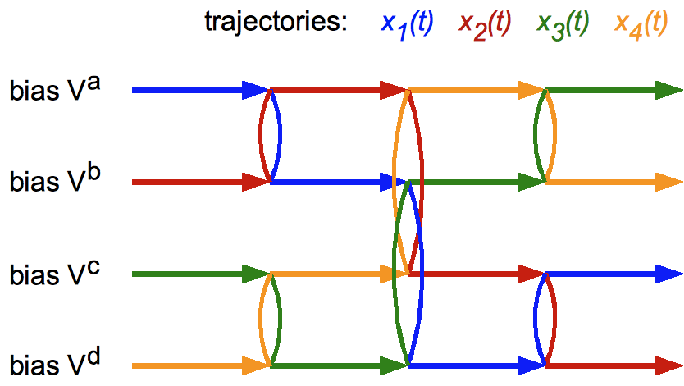
\includegraphics[width=9cm,angle=0]{./figures/be-scheme}
\caption{ Schematic representation of a bias-exchange simulation employing four replicas and four bias potentials. }
\label{be-scheme}
\end{center}
\end{figure}
%
Normally, in these conditions, each bias profile would converge very slowly to the
equilibrium free-energy, due to hysteresis. Instead, in the bias-exchange approach every fixed number of steps
(say 10,000) an exchange is attempted between a randomly selected pair of replicas $a$ and $b$.
The probability to accept the exchange is given by a Metropolis rule:
\begin{eqnarray}
\min\left( 1, \exp \left[ \beta ( V_G^a(x^a,t)+V_G^b(x^b,t)-V_G^a(x^b,t)-V_G^b(x^a,t) ) \right] \right)
\end{eqnarray}
where $x^{a}$ and $x^{b}$ are the coordinates of replicas $a$ and $b$
and $V_{G}^{a(b)}\left(x,t\right)$ is the metadynamics potential
acting on the replica $a$($b$).
Each trajectory evolves through the high dimensional free
energy landscape in the space of the CVs sequentially biased by
different metadynamics potentials acting on one CV at
each time (see scheme in Fig.~\ref{be-scheme}). 
The results of the simulation are $N$ one-dimensional
projections of the free energy, whose convergence is
monitored as usual: if the chosen CVs
describe all the slow degrees of freedom, after the filling time
each $V_G$ grows evenly.
In the following example, a bias-exchange simulation is performed on a Ala-Ala-Ala
peptide (zwitterionic form, in vacuum with $\epsilon=80$, force field amber03), using the four backbone dihedral angles as CVs (see Fig.~\ref{ala3}): 
$\psi_1$ = (N$^1$-C$^1_\alpha$-C$^1$-N$^2$), $\phi_1$ = (C$^1$-N$^2$-C$^2_\alpha$-C$^2$),
$\psi_2$ = (N$^2$-C$^2_\alpha$-C$^2$-N$^3$), $\phi_2$ = (C$^2$-N$^3$-C$^3_\alpha$-C$^3$).
%
\begin{figure}
\begin{center}
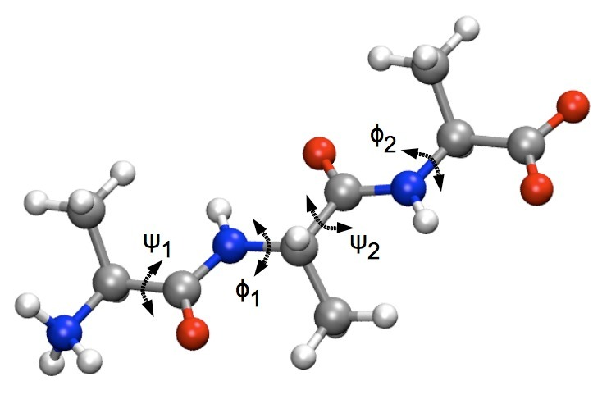
\includegraphics[width=9cm,angle=0]{./figures/ala3-dihedrals}
\caption{ Ala$_3$ peptide and dihedral angles used as CVs for bias-exchange metadynamics.}
\label{ala3}
\end{center}
\end{figure}
%
Four replicas of the system are employed, each one biased on a different CV,
thus four similar Plumed input files are prepared as follows:
%
\esempio{ 
first input file plumed0.dat for bias-exchange on Ala$_3$ \\ \\
{\tt
\# 1 kJ/mol (gromacs units) every 4 ps (timestep = 1 fs)	\\
HILLS HEIGHT 1.0 W\_STRIDE 4000					\\
PRINT W\_STRIDE 500						\\
BIASXMD								\\
								\\
\# psi1					\\
TORSION LIST  1  5 11 13 SIGMA 0.314	\\
\# phi1					\\
TORSION LIST 11 13 15 21 SIGMA 0.314	\\
\# psi2					\\
TORSION LIST 13 15 21 23 SIGMA 0.314	\\
\# phi2					\\
TORSION LIST 21 23 25 31 SIGMA 0.314	\\
					\\
\#NOHILLS CV 1				\\
NOHILLS CV 2				\\
NOHILLS CV 3				\\
NOHILLS CV 4				\\
					\\
ENDMETA					
}}
\esempio{ 
second input file plumed1.dat for bias-exchange on Ala$_3$ \\ \\
{\tt
\# 1 kJ/mol (gromacs units) every 4 ps (timestep = 1 fs)	\\
HILLS HEIGHT 1.0 W\_STRIDE 4000					\\
PRINT W\_STRIDE 500						\\
BIASXMD								\\
								\\
\# psi1					\\
TORSION LIST  1  5 11 13 SIGMA 0.314	\\
\# phi1					\\
TORSION LIST 11 13 15 21 SIGMA 0.314	\\
\# psi2					\\
TORSION LIST 13 15 21 23 SIGMA 0.314	\\
\# phi2					\\
TORSION LIST 21 23 25 31 SIGMA 0.314	\\
					\\
NOHILLS CV 1				\\
\#NOHILLS CV 2				\\
NOHILLS CV 3				\\
NOHILLS CV 4				\\
					\\
ENDMETA					
}}
\esempio{ 
third input file plumed2.dat for bias-exchange on Ala$_3$ \\ \\
{\tt
\# 1 kJ/mol (gromacs units) every 4 ps (timestep = 1 fs)	\\
HILLS HEIGHT 1.0 W\_STRIDE 4000					\\
PRINT W\_STRIDE 500						\\
BIASXMD								\\
								\\
\# psi1					\\
TORSION LIST  1  5 11 13 SIGMA 0.314	\\
\# phi1					\\
TORSION LIST 11 13 15 21 SIGMA 0.314	\\
\# psi2					\\
TORSION LIST 13 15 21 23 SIGMA 0.314	\\
\# phi2					\\
TORSION LIST 21 23 25 31 SIGMA 0.314	\\
					\\
NOHILLS CV 1				\\
NOHILLS CV 2				\\
\#NOHILLS CV 3				\\
NOHILLS CV 4				\\
					\\
ENDMETA					
}}
\esempio{ 
fourth input file plumed3.dat for bias-exchange on Ala$_3$ \\ \\
{\tt
\# 1 kJ/mol (gromacs units) every 4 ps (timestep = 1 fs)	\\
HILLS HEIGHT 1.0 W\_STRIDE 4000					\\
PRINT W\_STRIDE 500						\\
BIASXMD								\\
								\\
\# psi1					\\
TORSION LIST  1  5 11 13 SIGMA 0.314	\\
\# phi1					\\
TORSION LIST 11 13 15 21 SIGMA 0.314	\\
\# psi2					\\
TORSION LIST 13 15 21 23 SIGMA 0.314	\\
\# phi2					\\
TORSION LIST 21 23 25 31 SIGMA 0.314	\\
					\\
NOHILLS CV 1				\\
NOHILLS CV 2				\\
NOHILLS CV 3				\\
\#NOHILLS CV 4				\\
					\\
ENDMETA					
}}
%
Note that Plumed automatically enforces the periodicity of the CV {\tt TORSION}
between (-$\pi$,$\pi$) (e.g., when the system is close to $\pi$ it feels also the hills 
which were put close to -$\pi$).
The four replicas start from the same Gromacs topology file (even if it is not necessary), 
replicated four times
({\tt topol0.tpr, topol1.tpr, topol2.tpr, topol3.tpr}).
Finally, Gromacs is launched as a parallel run on 4 cores, with one replica per core, with the command 
\esempio{
{\tt mpirun -np 4 mdrun -plumed plumed -multi 4 -replex 5000} 
}
where {\tt -replex 5000} indicates that every 5000 molecular-dynamics steps
all replicas are randomly paired (e.g. 0-2 and 1-3) and exchanges are attempted
between each pair (as printed in the Gromacs {\tt *.log} files).
The frequency by which exchanges are attempted is a parameter of the simulation
which should be optimized for the specific problem at hand, but different
benchmarks show that the convergence of the simulation is robust with respect to it~\cite{cossio10jpcb}.

\subsection{Convergence of the simulation}

The convergence of the one-dimensional free-energy profiles (parallel growth)
can be monitored by plotting the sum of the hills at diferent times with the program {\tt sum\_hills.x}:
%
\esempio{
generate FES profiles from HILLS0 every 100 hills (important: -pi 1 declares a (-$\pi$,$\pi$) periodic range): \\
{\tt
sum\_hills.x -file HILLS0 -ndim 1 -ndw 1 -stride 100 -pi 1 \\
}
\\
plot the FES profiles fes.dat.1, fes.dat.2, etc.: \\
{\tt
xmgrace fes.dat*
}}
%
The parallel growth of the bias profiles at different times for each CV 
is an indication that the simulation is converged.
However the best final estimate of the free energy profile is obtained by averaging
the instantaneous bias profiles after the filling time: 
\begin{eqnarray}
 F(s) \approx -\frac{1}{t-t_F}\int_{t_F}^t dt \ V_G(s,t)
\end{eqnarray}
as discussed in Ref.~\cite{gerv-laio09review,marinell-crespo10}.
This can be simply done with the option {\tt -aver} of {\tt sum\_hills.x}, e.g. making
an average over the last 500 hills:
\esempio{{\tt
  sum\_hills.x -file HILLS0 -ndim 1 -ndw 1 -pi 1 -aver 500
}}
The resulting estimate of the FES profile can be finally compared to the files {\tt EQUIL\_FESx} which contain
the "exact" FES computed from a very long (3~$\mu$s) equilibrium MD simulation without any bias (Fig.~\ref{be-validation}).
In the latter case the free energy along each dihedral angle is simply obtained as 
$F(s)=-k_BT\log(p(s))$, with $s$ a dihedral angle.
As one can notice, the agreement is excellent (at a fraction of the computational cost!), 
and the bias-exchange profile has a smaller uncertainty
on the barriers as there the equilibrium simulation has a very poor sampling.
%
\begin{figure}
\begin{center}
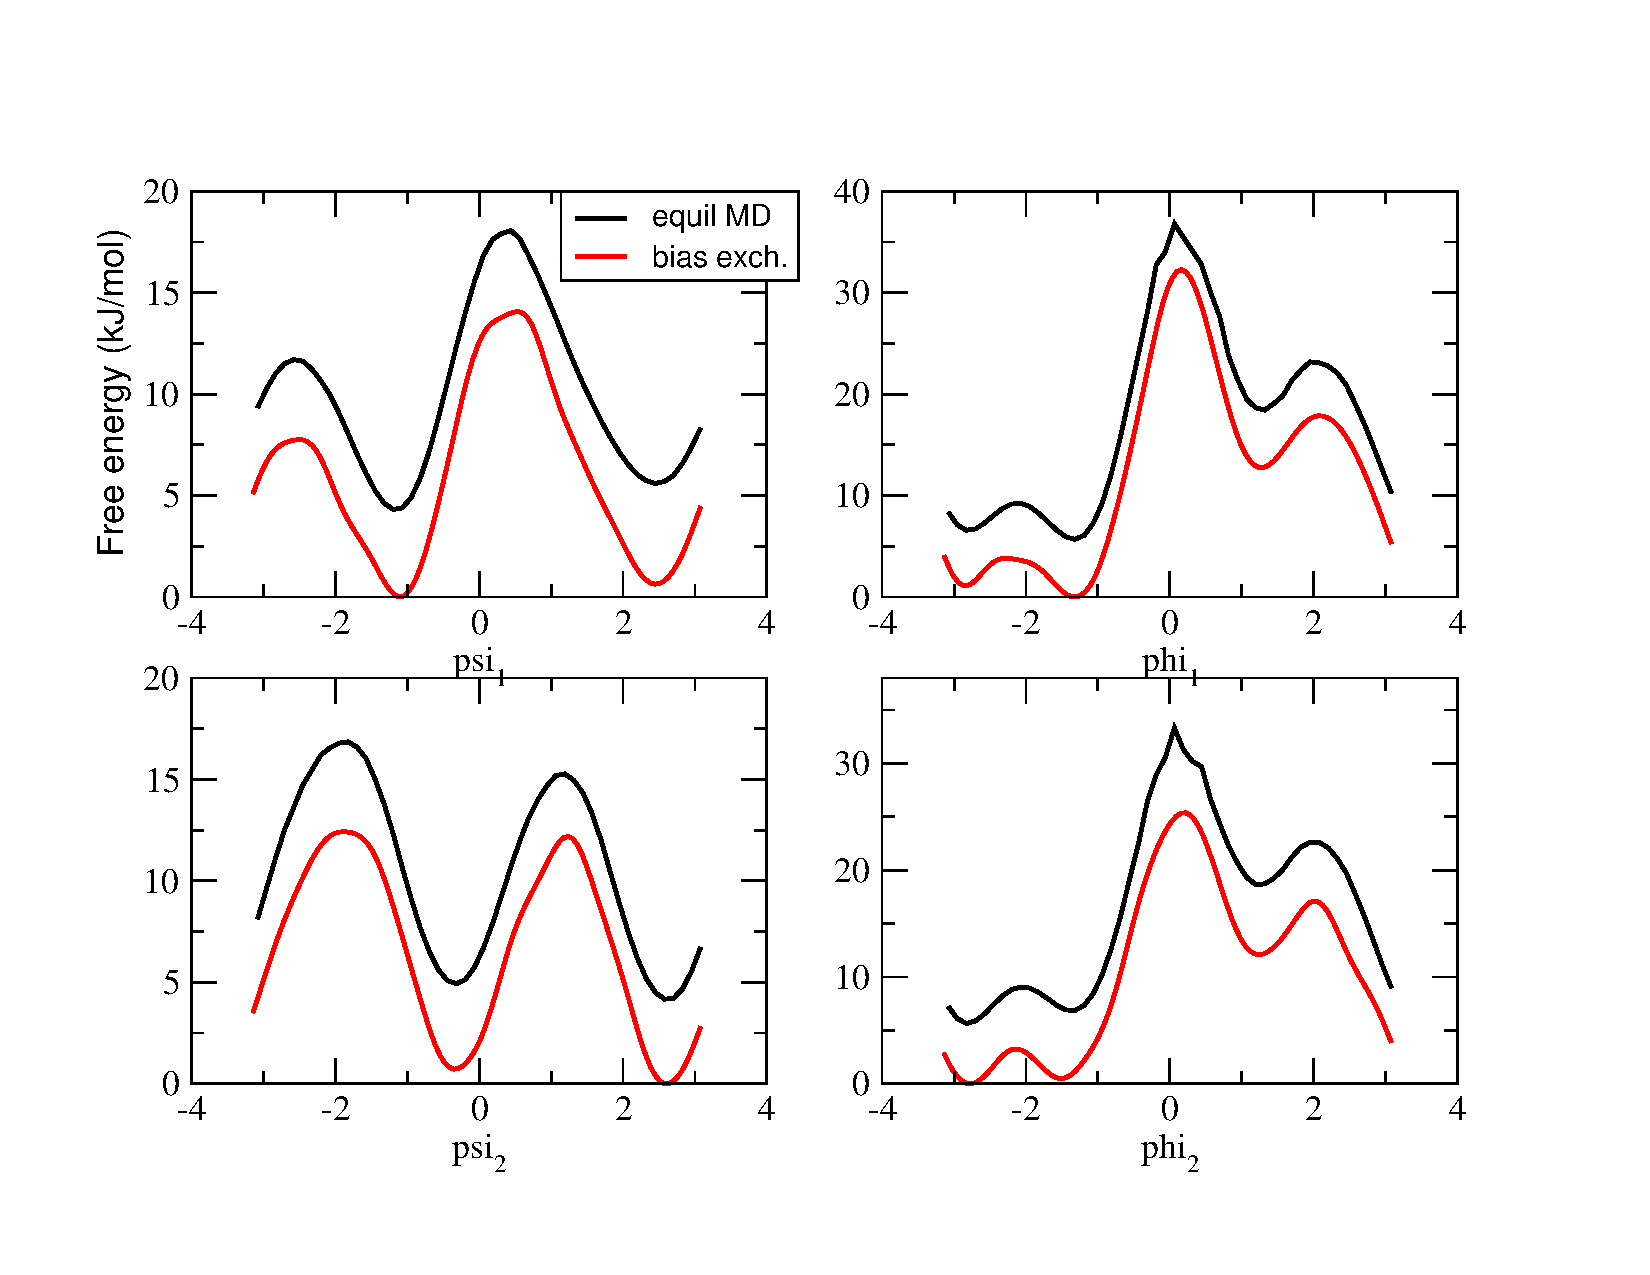
\includegraphics[width=14cm,angle=0]{./figures/be-validation}
\caption{ Comparison of Ala$_3$ free-energy profiles obtained from bias-exchange (4 replicas running for 4~ns) and from equilibrium MD
(3~$\mu$s).}
\label{be-validation}
\end{center}
\end{figure}
%

An important feature of the bias-exchange technique is that, provided good CVs are employed,
the computational cost scales approximately linearly with the number of CVs, even if the volume
of the CV-space grows exponentially: this can be easily verified increasing the length of the
peptide to Ala$_4$, Ala$_5$, etc. and using the 6, 8, etc. backbone dihedrals as CVs.
In this case, using a proportional number of CPUs the simulation time per replica remains similar.
However, as for all enhanced sampling techniques, very complex systems with a large number of metastable
states (e.g., folding a protein of say 60 amino acids) represent a major challenge.

The output files of the bias-exchange simulation can be also used to reconstruct
the fully four-dimensional free-energy landscape employing the weighted-histogram technique,
as explained in Section~\ref{bewham}.

\chapter{Advanced techniques}
\section{Path based collective variables}
Path collective variables (PathCV) are very useful whenever one wants to find an optimal free energy channel
connecting two specific regions in the phase space and calculate the associated free energy profile.
Typical examples where the use of pathCV is beneficial are docking/undocking of a ligand from
a target, complex chemical reactions and conformational changes in biomolecules.  
Whether or not ``two specific regions'' can be defined for an initial state and a final state depends 
on the nature of the system under study and the choice of the subspace in which the path is defined 
(coarse graining).
For example one could think that the folding of a peptide is not a suitable case for pathCVs as the `
`folded'' state is easily defined, but the ``unfolded'' generally includes several different states. 
However, by suitably ``remapping'' the space in which the path is defined
also the unfolded state may be univocally defined.
A good choice for folding could be the use of the number of native hydrogen bonds.
In this case the folded state would be the sate with the maximum number
of native-like hydrogen bonds, while the unfolded state would have no hydrogen bonds. 
The folding paths in this space will be all the energetically favorable 
changes of hydrogen bond patterns connecting the unfolded state to the unfolded state.\cite{Juraszek:2007p15828}
The level of coarsening in defining the path (i.e. the definition of the subspace
in which the path is defined) has to be decided by the user according 
to its chemical intuition and it is not always easy.

A given point in the Cartesian space corresponds to a vector ${\bf
  \Theta}(x)$ in the coarse grained space (adopting the notation of
Maragliano/Vanden-Eijnden). In particular the components of this
vector are defined with $\theta_m(x)$, namely:
\begin{eqnarray}
{\bf \Theta}(x)=(\theta_1(x),\theta_2(x),\ldots,\theta_N(x) )
\end{eqnarray}
where $N$ is the number of coarse grained variables needed to simulate a given process.
For example, in a chemical reaction it might turn to be useful to describe the reaction in terms of  some h-bond distances and specific angles. Each of these is one $\theta_m(x)$. 
In \plumed\ the choice is (so far) limited to three possibilities: \keyword{RMSD}, \keyword{DRMSD} and \keyword{CMAP}.
In RMSD the representation of the configuration is done in terms of
explicit Cartesian coordinates of the subset of atoms involved in the CV. In the \keyword{DRMSD}
each configuration is represented in terms of a set of specific
distances. In the \keyword{CMAP} representation each configuration is
represented in terms of a set of contacts (whose value depends on
specific distances through a tunable switching function).
%It is possible to judge if the choice of the subspace in which the
%path has been effective or not.
%% The most effective and intuitive is performing a ``committor analysis'' and a ``committor distribution''. 
%% The first is, for a given set of collected snapshot at a given point along the path, the probability to fall into the reactant state before falling into the product state. This quantity provides the  The second is generally calculated at the transition state and is the probability that a single configuration falls in the reactant before falling into the product state. Please refer to suitable literature on how to perform these calculations \cite{Bolhuis:2000p8198,Ren:2005p5706,Maragliano:2006p6867,Mantz:2009p12678}.  


%% A reaction pathway can be described as a parametric vectorial function that moves from the reactant to the product in this coarse-grained space that depends on a parameter $0<\alpha<1$.
%% \begin{eqnarray}
%% {\bf \Theta}_{path}(\alpha)=(f_1(\alpha),f_2(\alpha),\ldots,f_N(\alpha) ).
%% \end{eqnarray}
Once the subspace in which the path is defined has been chosen, a
reference path in this subspace must be defined. 
In \plumed\ the reference path is defined in terms of a number $M$ of points (called ``frames'') along this parametric functions, say:
\begin{eqnarray}
{\bf \Theta}_{path}(i)=(f_1(i),f_2(i),\ldots,f_N(i) ).
\end{eqnarray}

The number of frames defining the path depend on the length scale of the process.
An important consideration is that the frames must be as equally spaced
(in the current metric) as possible. \plumed\ can run
with paths whose frames are unequally spaced, but this can result is a
poor reconstruction of the free energy profile. 

Once a reference path is defined (see also below) two collective
variables can be calculated in \plumed\. The first returns the projection
of the current phase-space vector on the reference path.
This tells us if we are closer to the reactant state, or to the
product state or if we are somewhere in between.
This CV is defined as it follows:

\begin{eqnarray}
S(x,\{{\bf \Theta}_{path}(m)\}_{m=1,M})=\frac{\sum_i i\ \exp{- ( \lambda| {\bf \Theta}_{path}(i) - {\bf \Theta}(x) | )}}{   \sum_i \ \exp{- ( \lambda| {\bf \Theta}_{path}(i) - {\bf \Theta}(x) | )}   }
\end{eqnarray}
that is a function which returns a fractional corresponding to the
closest point along the path. If the closest point is 2 then its
exponential will be larger respect to the other ones and therefore the
CV will have a value close to 2.
However, the progress along this CV alone can be misleading. If our
system is very far from the pre-defined path or if it takes a
tangential path, we might still see that $S$ smoothly varies from 1 to
M while in reality it is following a different path.
For this reason is very useful to measure a distance from the
reference path, defined as it follows:

\begin{eqnarray}
Z(x,\{{\bf \Theta}_{path}(m)\}_{m=1,M})=-\frac{1}{\lambda}\ln \sum_i \ \exp{- ( \lambda| {\bf \Theta}_{path}(i) - {\bf \Theta}(x) | )}
\end{eqnarray}
which is the distance along the path. Consider once again the case that one exponential is larger than the other then it is easy to retrieve from the formula the distance of the closest frame. 

Now we can discuss how the parameter $\lambda$ is chosen and how a good 
set of frames $\{{\bf \Theta}_{path}(m)\}_{m=1,M}$ defining the
reference path is found.
Our rule of thumb for $\lambda$ is to use the following formula:
\begin{eqnarray}
\lambda=2.3/<|{\bf \Theta}_{path}(i)-{\bf \Theta}_{path}(i+1)| >.
\end{eqnarray}
The reason for that is simple. The $S$ variable should change \underline{smoothly}
from a frame to another. To obtain this effect the exponentials
centered on each of the M frames must overlap. That is, 
even if you are precisely on one frame,  the tails of the neighbor 
exponential must not vanish. If any two frames are 
distant $\Delta$ in our subspace, we want to 
tune lambda so that the exponential value of the neighbor is around
0.1. 
\begin{eqnarray}
0.1=\exp (-\lambda \Delta)
\label{lambdatrick}
\end{eqnarray}
which, by inversion, gives exactly the value reported above. 
If you are not able to find a set of frames that
have a uniform spacing then you must calculate the value of 
\keyword{LAMBDA} according the largest
inter-nodal spacing. This might limit the resolution 
the reconstructed free-energy profile.


Another important consideration is that the frames should reproduce a parametric
curve in a reliable way. That is, the closest neighbors to point $i$ in the sequence
 (which are $i-1$ and $i+1$) must be the closest also in the chosen space.

\begin{equation}
|{\bf \Theta}_{path}(i)-{\bf \Theta}_{path}(i+1)|=|{\bf \Theta}_{path}(i)-{\bf \Theta}_{path}(i-1)|<|{\bf \Theta}_{path}(i)-{\bf \Theta}_{path}(j)|
\end{equation}
with $j<i-1$ or $j>i+1$ and
\begin{equation}
|{\bf \Theta}_{path}(i-1)-{\bf \Theta}_{path}(i+1)| \simeq 2|{\bf \Theta}_{path}(i)-{\bf \Theta}_{path}(i-1)|.
\end{equation}
This last condition can be difficult to fulfill if we are in a
non-euclidean space. Sometimes it helps to  add more points along the
path.

To judge how good is the parameterization of the path we can visualize 
the all-against-all frame distances in the chosen subspace.
\\
%begin{figure}[here]
%\begin{center}
%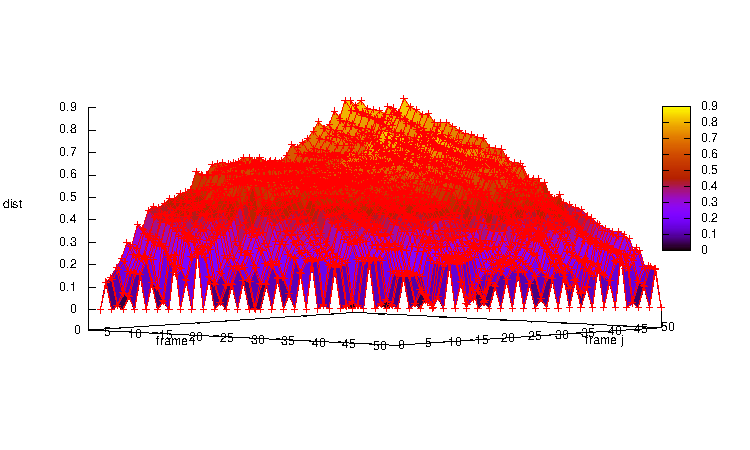
\includegraphics[width=10cm,angle=0]{./path/badparam}
%\caption{An example of bad parametrized path}
%\end{center}
%\end{figure}
%
%\begin{figure}[here]
%\begin{center}
%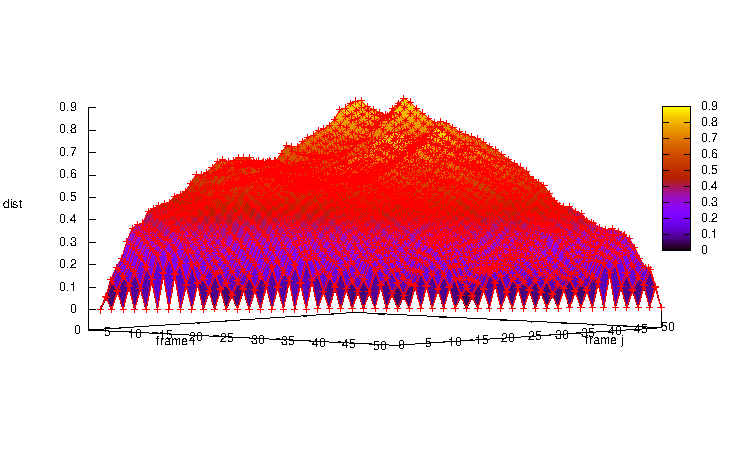
\includegraphics[width=10cm,angle=0]{./path/goodparam}
%\caption{An example of well parametrized path}
%\end{center}
%\end{figure}
\begin{tabular}{ l | c  }
 Badly parameterized path & Well parameterized path\\
 \hline\\
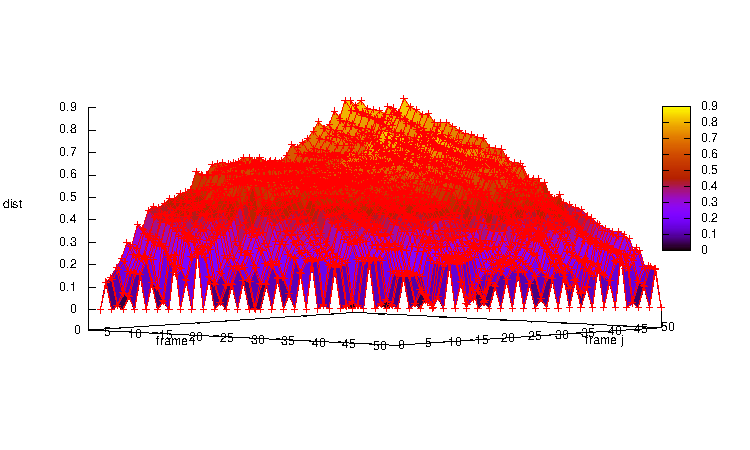
\includegraphics[width=7cm,angle=0]{./path/badparam}\label{badparam}  & 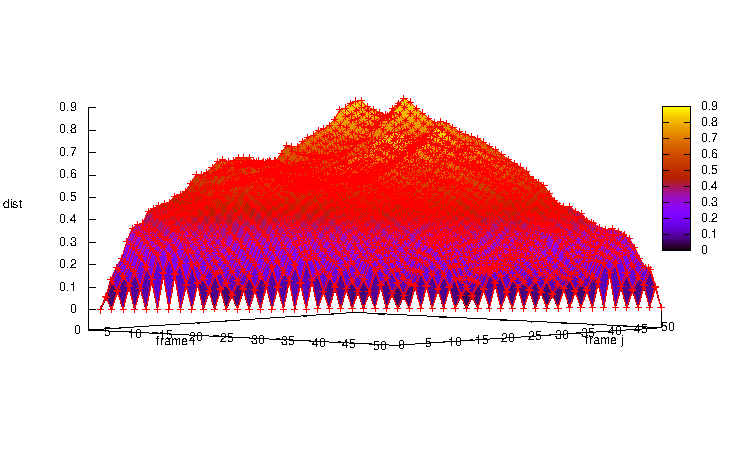
\includegraphics[width=7cm,angle=0]{./path/goodparam}\label{goodparam}
\end{tabular}
In Fig. \ref{badparam} it is evident that the distance of each frame
with its neighbors is very bad (the diagonal elements are irregular
and their distance changes a lot along the path) while in
\ref{goodparam} the diagonal elements are much better spaced and
uniform along the path. The way to produce a well parametrized path
may vary a lot. 
The simplest choice is to just take a set of equally spaced frames
along a straight line connecting the initial and final state.
This choice, albeit it is simple, has some drawbacks as we will 
see in the first exercise.
A more systematics choice is to select
the frames  from a trajectory produced with \plumed\  using a 
steered MD or targeted MD simulations. This will ensure that the frames
that you use correspond to accessible states in the phase space. Out
of this set you can choose the most equidistant points along the path via a
Monte Carlo procedure. This is an effective but ad-hoc solution. We
recommend you to find your own effective protocol that will be be system
dependent.

A different possibility is to use the finite temperature
string method procedure described in Ref. \cite{Maragliano:2006p6867}.
It produces equidistant frames. But it has the drawback of not
taking into account the curvature of the space and moreover it may
produce fictitious interpolated points that may not correspond to
physical situation.


Another important point is the choice of the ``metrics''. This means
the way in which we calculate the distances $| {\bf \Theta}_{path}(i)
- {\bf \Theta}(x) |$ . The adopted metrics in \plumed\ depends on the
chosen representation. For example, in the \keyword{RMSD}
representation the distance between the running simulation frame and
one reference frame is calculated as a sum of the distances squared
after optimal alignment of the two structures through
Kearsley\cite{kearsley} alignment method. In case of \keyword{CMAP} it
is performed by summing up the difference in contacts between  the
reference and the running frame, squared and similarly in
\keyword{DRMSD} the sum of the differences (squared) between two
different set of distances (running frame vs one of the references)are
calculated.

\plumed\ does not yet implement a general scheme for mixing variables
because one one side these could be rather tricky due to the inherent
difficulty of managing different CVs within one single CV but on the
other side you might think that this can offer a safe approach to the
users (and tested).
If you are interested in all the tricks behind a general variable
which is function of other variables please refer to
\cite{Maragliano:2006p6867}.


Now, let's come to the more practical part of this section.
\subsection{Metadynamics on a sub-optimal path}
The first exercise that we propose is to try is a metadynamics run
with pathCV on a path that does not correspond to a ``low-free energy channel''.
Out of time consideration, we will make use of alanine dipeptide for
this example.

Its free energy landscape is conveniently represented 
by two angles that are called Ramachandran angles and are generally useful because specific secondary structures of protein
present specific combinations of these two dihedrals. The plot of these two dihedral is called ``Ramachandran plot''.
A free energy for this small peptide as function of these two dihedrals resembles the one showed in \ref{ramapaths}.
It is visible a pathway that leads to a minima which is located at $\Phi\simeq-2.6, \Psi\simeq2.8$ which is called $C_{ax}$ and another one located at 
$\Phi\simeq1, \Psi\simeq-0.5$ which is connected to another minimum called $C_{eq}$.
\begin{figure}[here]
\begin{center}
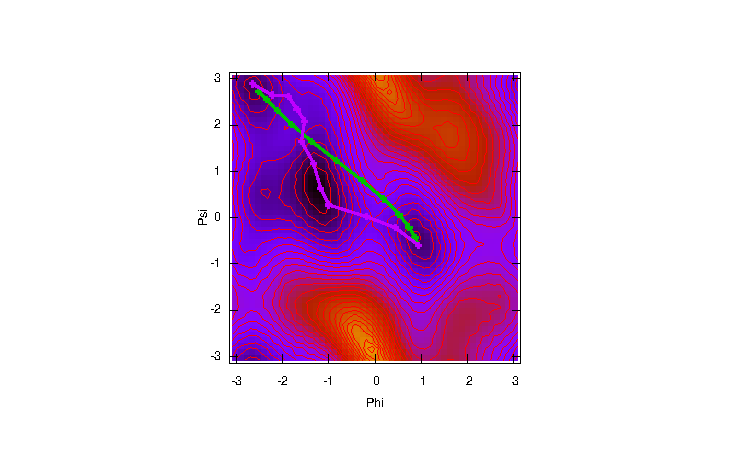
\includegraphics[width=\textwidth,angle=0]{./path/umbrella_sampling/rama_paths}
\caption{The free energy landscape of an alanine dipeptide with the GROMOS96 all\-atom force field. Iso-lines are drawn every 1kcal/mol. Two paths are traced. A  "bad" path is in green and is obtained by straight interpolation. In pink an optimized path is shown. }
\label{ramapaths}
\end{center}
\end{figure}

Let's assume that those two minima are known. In this case one could naively imagine that the typical pathway would be something that leads from
$C_{ax}$ to $C_{eq}$ via a linear path. This means that we can take a linear interpolation of the Cartesian coordinates that go from the reactant ($C_{ax}$) to the product state ($C_{eq}$)  and simply assume this as a reactive pathway (see green pathway in Fig. \ref{ramapaths}).  Of course we can immediately imagine that, although the two extrema are stable and low energy, some intermediate states are rather unhappy to lie there and we might expect to find an energetic funnel which is not running all the way close to the initial guess.
In \plumed\ the input for path collective variables is as follows:
\esempio{
The following is an example of input file for a path collective variable run. \vspace{10pt} \\
{\tt
PRINT W\_STRIDE 100 \\
\#\\
\# a rather rude metadynamics. do not take this as production conditions\\
\#\\
HILLS W\_STRIDE 200.0 HEIGHT 0.4 \\
\#\\
\# the two path variables
\#\\
S\_PATH TYPE RMSD FRAMESET frame\_ NFRAMES 12 LAMBDA 10300 SIGMA 0.3  \\
Z\_PATH TYPE RMSD FRAMESET frame\_ NFRAMES 12 LAMBDA 10300 SIGMA 0.002 \\
\#\\
\# additional ramachandran variables might be useful to understand what is happening\\
\#\\
TORSION LIST 5 7 9 15   \\
TORSION LIST 7 9 15 17 \\
ENDMETA \\
}}
The syntax for path collective variables consists of a initial directives \keyword{S\_PATH} or \keyword{Z\_PATH}. 

\keyword{S\_PATH} is the CV that gives the progress along the path while   \keyword{Z\_PATH} gives the distance from 
the path itself. Then a keyword is required that is the \keyword{TYPE} followed by the type. In this example is \keyword{RMSD} and this determines
the format for the input that one has to provide. In this case it is a simple pdb format. In this particular type it is very important that the
index in the second column of the pdb correspond to the absolute indexing within the program. For example, in NAMD the indexing must correspond to that of the same atoms in the formatted \*.coor. In SANDER I dump a pdb from the restart or coordinate file with ptraj and use that indexing. 
Similarly in GROMACS I use trajconv and dump a pdb and use that indexing. Generally it works. Labels and residue name and number can be different from the original one because \plumed\ is not aware of those information to double check (in many programs there are not easy to retrieve).    
A last note for the {\tt RMSD} keyword. The last column of the pdb (generally beta and occupancy) are here used to specify the weight to use in the alignment and the displacement. For example, consider a case of protein-ligand docking: in this case you want to measure the progress of the detachment of the ligand from the target by using the protein as reference system. In this case the atoms of the protein have to be included in the beta column with a value of 1.00 while the atoms of the ligand should be marked with a 0.00. The fact that the only thing that one wants to measure are the atoms of the ligand are denoted by reporting a 1.00 for the atoms of the ligand in the occupancy column while putting the atoms of the protein used for of the alignment to 0.00. It is also allowed to use the same atom for alignment and the measure.  
The \keyword{LAMBDA} determines the fudge factor for the summation of the exponential for the formulas of the path. See equation \ref{lambdatrick} and note that in GROMACS the units are $nm^2$ (quite common pitfall!!!). 
This example is performed  with GROMACS. Note that in case of \keyword{RMSD} it is much better you use the double precision version of the code.
Therefore it consists in the following steps. 
\begin{itemize}
\item Modify the md.mdp (which is the GROMACS input parameter file) according to your needs. Here is the point where you should provide the number of steps. Note that in this case we use fully flexible hydrogens and no constraints on them. This is an accepted standard for alanine dipeptide.
\item Generate the {\tt topol.tpr} via {\tt grompp} GROMACS preprocessing program. This file is the only one needed to run a plain run with {\tt mdrun}. In case of a run with \plumed\ you should specify that you use \plumed\ at runtime and use the input reported above. For example it is likely that 
by running {\tt mdrun -plumed metadyn} (where{\tt metadyn.dat} is the metadynamics input file reported above) will work if your {\tt mdrun} version is 
compiled with \plumed\ .
\end{itemize}
The script file is therefore something like this
\esempio{{\tt
grompp -f md.mdp -c 2ala.gro -p gromacs.top  \\
mdrun -plumed metadyn
}}
I find personally very helpful to have a look to the {\tt COLVAR} file and {\tt HILLS} file while are being produced. Just by asking yourself if what 
you see is what you expect you can double check if your input file is correct.
What you might see from this experiment is that {\tt COLVAR} (column 2:3, plot with gnuplot and a command like {\tt plot "COLVAR" u 2:3 w p })
you have a plot like the one reported below in Fig. \ref{colvar1_wrong}.
\begin{figure}
\begin{center}
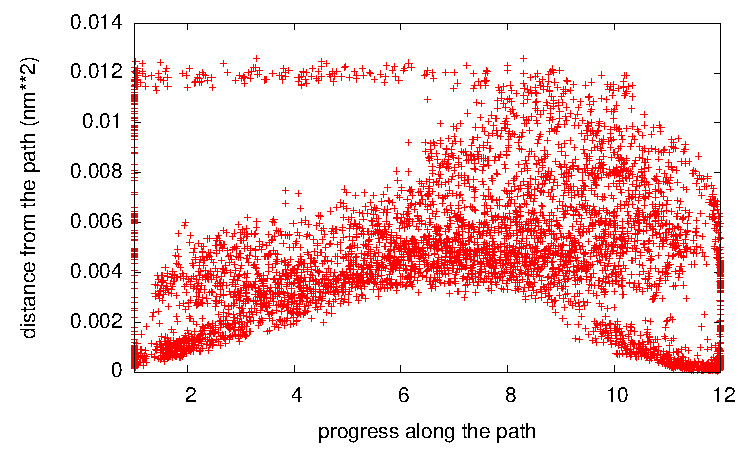
\includegraphics[width=10cm,angle=0]{./path/colvar1_wrong}
\caption{Progress and distance from the path in case of wrong path. The system does not follow the path closely but most of time is spent far away from the guess path.}
\label{colvar1_wrong}
\end{center}
\end{figure}


Another additional test you could try to do yourself is to try to reduce the \keyword{LAMBDA} of a couple of orders of magnitude and try to increase it.
What do you observe? (Large \keyword{LAMBDA} "atomize" regions together and hills width become strongly anisotropic. Small value lump all the space as it was one. Is this expected? Give a look to the equations of path CVs to make up your mind about that).

An important observation, the most important of all, is that for most of the progress along the path your system does not follow the path closely (Ideally the system follows the path when most of time stays at distance of the path$\simeq0$). This is crucial because it underlines that the guess pathway does not reproduce the reactive event as imagined. Fine, but you see the transition. So why bother? The fact is that states (and transition states) at large distance from the path include a number of structures that may be quite diverse. Therefore the transition state you might get is not composed of structures that have 0.5 probability of falling into the reactant before falling into the products (which is a "coarse" but correct definition of dynamical transition state). The result is that the free energy can be lower than expected from the experiment (because you lump in the TS a set of states that may be pre and post TS which, by definition, have lower energy). For these reason, whenever your system does not like to walk right on your path, please be suspicious and consider to adopt an improved version of the path (more about how to obtain it below).
\subsection{Metadynamics on a correct path}
What happens when the path is almost good? In this example we do the same exercise as done previously (same input files. Just minor modifications) but on an improved pathway (the pink one in Fig. \ref{ramapaths}) .
In case you change the pathway there are different options. One of that is just substitute the old reference files for the guess path  (in the previous
example their name was {\tt frame\_1.pdb}, {\tt frame\_2.pdb}, $\ldots$, {\tt frame\_12.pdb}) and remember to change the \keyword{LAMBDA}. This 
is mandatory because if the path changes but the number of guess point changes it is likely that the internodal distance change as well and the 
factor \keyword{LAMBDA} should be recalculated with the equation \ref{lambdatrick}. In this case  \keyword{LAMBDA}  is 3800 that is a signal that now the pathway is longer.
By repeating the same metadynamics calculation as before then you find a different landscape that is much better in that the path is strongly followed by the system during the metadynamics as an equivalent plot of the {\tt COLVAR} file points out.
\begin{figure}
\begin{center}
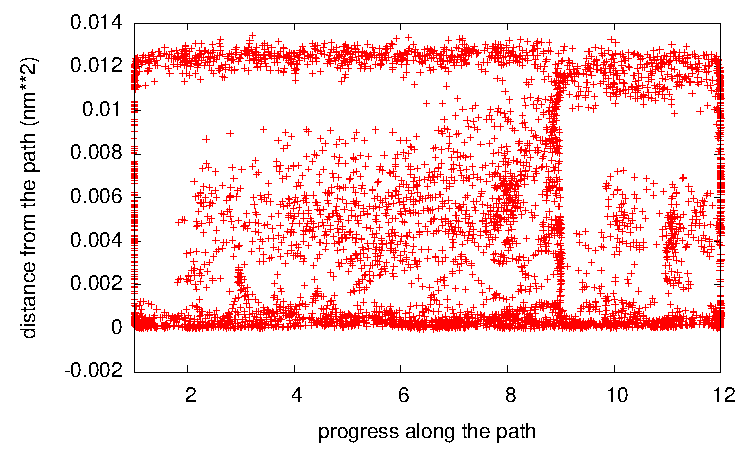
\includegraphics[width=10cm,angle=0]{./path/colvar1_good}
\caption{Progress and distance from the path in case of a correct path. The system does now follow closely the path.}
\label{colvar1_right}
\end{center}
\end{figure}
As you might expect now, the plot you obtain is pretty similar to the one you obtained before. It is just a "deformation" of it. This is rather important.
Path collective variables may create "ad-hoc" foliation of the space in an adaptive way and allow you to have many different representation, depending on your ability of retriving a good guess pathway. 

Now that the system follows more closely the guess path you may hope that, by performing a committor analysis on the TS this gives a value of 0.5 and you can really trust your transitions state. Try to figure out, from the Fig. \ref{ramapaths}, why you see all those pathways and how you can "map" them onto ramachandran plot so to double check if what you see is just an effect of the projection of the states on the PCVs or those pathways you see have an equivalent on the Ramachandran plot. How is it possible that a periodic representation on the Ramachandran plot is now "unfolded" in a
not periodic representation?

Finally, the cherry on the cake. Do a free energy with the usual command. {\tt sum\_hills  -ndim 2 -ndw 1 2 -ngrid 100 100  -file HILLS }
Before doing that, if you want to obtain meaningful results, you would be better to increase deposition time and simulation time as well.
Three nanoseconds should be sufficient.
The other way is to limit the path on the distance along the path and then limit the exploration only to the optimized region. This is reasonable as, for the reasons explained before, the regions at large distance are not well resolved. In this case we can still limit ourselves to just 100ps.
A possible input can be something like this:
\esempio{
The following is an example of input file for a free energy calculation along the path in a limited region of the path itself. \vspace{10pt} \\
{\tt
PRINT W\_STRIDE 100 \\
\#\\
\# a rather rude metadynamics. do not take this as production conditions\\
\#\\
HILLS W\_STRIDE 400.0 HEIGHT 0.4 \\
\#\\
\# the two path variables: metadynamics only on S\_PATH, the other is just for monitoring\\
\#\\
S\_PATH TYPE RMSD FRAMESET frame\_ NFRAMES 12 LAMBDA 10300 SIGMA 0.25  \\
Z\_PATH TYPE RMSD FRAMESET frame\_ NFRAMES 12 LAMBDA 10300  \\
\#\\
\# A wall over Z can be useful to limit the orthogonal exploration and speed up convergence\\
\#\\
U\_WALL CV 2 LIMIT 0.0 KAPPA 100.0 \\
\#\\
\# additional ramachandran variables might be useful to understand what is happening\\
\#\\
TORSION LIST 5 7 9 15   \\
TORSION LIST 7 9 15 17 \\
ENDMETA \\
}}
At the end you can integrate simply with the usual command {\tt sum\_hills -ndim 1 -ndw 1 -file HILLS} you can retrieve the 
free energy file {\tt fes.dat} that you can easily plot with gnuplot and the command {\tt p "./fes.dat" u 1:(\$2/4.186) w lp}. Note that the factor 4.186
is the kJoule to kcal conversion factor as the GROMACS internal energy units (and therefore hills height) are in KJoule/mol. 
What can you see? Can you compare with the free energy along the pink path in Fig. \ref{ramapaths}? Are you getting something you are expecting?

{\bf \underline{Now a final important remark} }. A very important point in understanding how to choose path collective variables is the choice of the metrics. In \plumed\ you have the choice between \keyword{RMSD},\keyword{DRMSD} and \keyword{CMAP}. However one can be tempted in simply producing an artificial path via  \keyword{TARGETED} and then using the frames as an input for pdbs for the type \keyword{RMSD}.
This is not always the best choice (very often it is not at all). Consider carefully your problem. If you expect large entropic basins probably something like \keyword{CMAP} is good for you as the degeneracy does not increase so dramatically as function of the distance from the path as for \keyword{RMSD}. The \plumed\ developers team is working on a flexible scheme for introducing a flexible scheme for adopting a complete flexible metrics.
A good reference could be \cite{Bo.Bra:08} where we had to use two different metrics depending on the transition that we wanted to do. 

\subsection{Path optimization}
An important question is how to obtain and improve the reference path.
There are a number of ways to perform this task and a
detailed treatment goes far beyond the scope of this tutorial. Anyway
it is quite important to provide pointers to some relevant literature
and briefly discuss the main issues that one might encounter.
Historically path optimization was first performed in small molecules in electronic
structure calculations.

In this regime, if the number of atoms is small (around 10-20 atoms),
then it is possible to do a guided search on the potential energy
surface (PES) and find the saddle point. This is in generally not
completely automatic and requires some knowledge on the system to
define some "meaningful" set of additional coordinates (called
"redundant coordinates") that would increase the possibility of
finding a saddle point on the PES. The saddle point is defined as the
point in the configurational space that has zero force and whose
Hessian matrix (the matrix of the second derivatives of the energy
respect to the positions) has positive eigenvalues but one. That
specific negative eigenvalues is associated to an eigenvector that,
when followed in two opposite directions, joins the reactant and the
product. This is a standard strategy that is based on saddle point
search and intrinsic reaction coordinate following which is
implemented in many codes, among which the popular Gaussian
code. However this approach has some severe limitations. First, when
scaling up the number of atoms (with a solvent layer), this procedure
becomes inefficient as many minima may interfere and the saddle point
search may be stuck on non-useful unreactive saddle points. Moreover in
this regime the free energy is hardly obtained with the rigid rotor
approximation and many non-harmonic effect start to appear. similarly,
adding another redundant coordinate might be of limited help
because as the number of atoms increase, cooperatively starts to
appear. These issues have been addressed with the 
"Nudged Elastic Band" (NEB) \cite{neb0,neb1,neb2} approach where many
replica of the same system, each one in a chain of guess states that
go from the reactant to the product, are evolved together and each
replica is chained to the next replica by a spring which keep each
replica equidistant from the other (the so called "re-parametrization
force").

It works well at T=0 K for chemical reaction. Here the trick
is that in this way the path is "forced" to make the reaction and
therefore one can find the closest local minima to the input guess
path thus avoiding the situation in which the saddle point is found
but it does not connect reactant and products. \\
What about T$>$0 K? In the recent years many techniques were
introduced were the main task is, instead minimizing the path on the
PES, one wants to minimize the path using the FES. The best known is
the so-called "Finite temperature string method" 
\cite{ftstringmethod,dialastringmethod,maragliano} . This technique
can be easily implemented with \plumed\ as it follows: create a number of replicas of the
system along the path and put some umbrella on \keyword{S\_PATH} on
the nodal points (say 1.0, 2.0, 3.0, etc\ldots) and a
\keyword{U\_WALL} on 

\keyword{Z\_PATH} so that each point does not escape
dramatically. Then you might collect configurations and average them
so to extract a new path. Re-parametrization requires some care and an
ad-hoc code should be written for reparametrizing each metrics
(Cartesian coordinates require optimal aliened in a correct way while
angles require that correct periodicity is applied). Please refer to
\cite{maragliano}. Another technique I have been applying is to use
the NEB chain of springs \cite{neb0,neb1,neb2} to produce an
additional reparametrizing force and then evolve in a steepest descent
fashion. For this approach please refer to \cite{brand07}.

Another possible approach is to performe a slow steered MD in
slow regime with a limit on \keyword{Z\_PATH} and then resorting the
new frames from the trajectory. However the path found can be suboptimal
if you pull too fast. 

\section{Variables for secondary structure in proteins}
%fabio

Many fundamental protein processes like folding, unfolding or misfolding to a pathological form involve transformations of the secondary structure.
If we define the $\phi$ and $\psi$ backbone dihedral angles as formed by atoms (C$^1$-N$^2$-C$^2_\alpha$-C$^2$) and (N$^1$-C$^1_\alpha$-C$^1$-N$^2$)
respectively, then alpha secondary structure is localized in a region around (-60$^\circ$,-45$^\circ$) in the ($\phi$,$\psi$) Ramachandran plot,
whereas beta is in a region around (-135$^\circ$,+135$^\circ$) (see Fig.~\ref{secstr}-a).
Both alpha helix and beta sheet are characterized by hydrogen bonds between the backbone C=O and N-H groups of different amino acid residues.
In helices the hydrogen-bonded residue pairs are of the type $(i,i+n)$, $(i+1,i+n+1)$, $(i+2,i+n+2)$, etc., where $n$ = 3, 4, or 5.
Beta sheets are characterized by similar pairs as alpha but with larger $n$ (parallel beta) or by pairs $(i,i+n)$, $(i-1,i+n+1)$, $(i-2,i+n+2)$,
etc., with $n>4$ (antiparallel beta). Further, the side chains of neighboring amino acids have a typical stacking: in the alpha helix they point outward, 
in the beta sheet they form pairs which are alternatively above or below the sheet.

In Plumed there are several CVs which can induce changes of secondary structure based on the previous
structural features:
the H-bonds (CVs {\tt COORD}, {\tt HBONDS}), the typical dihedrals (CVs {\tt TORSION}, {\tt DIHCOR}, {\tt ALPHABETA}), or the detailed
chain conformation (CVs {\tt ALPHARMSD}, {\tt ANTI/ PARABETARMSD}). Here we will illustrate only the CVs {\tt ALPHABETA}
and {\tt xRMSD}.
As protein model we consider a poly-valine peptide Val$_{20}$ in vacuum (with ACE/NME capping groups, 
amber03 force field)
as it allows to obtain realistic secondary structure: valine has a volume which is the average of all amino acids. 

\begin{figure}
\begin{center}
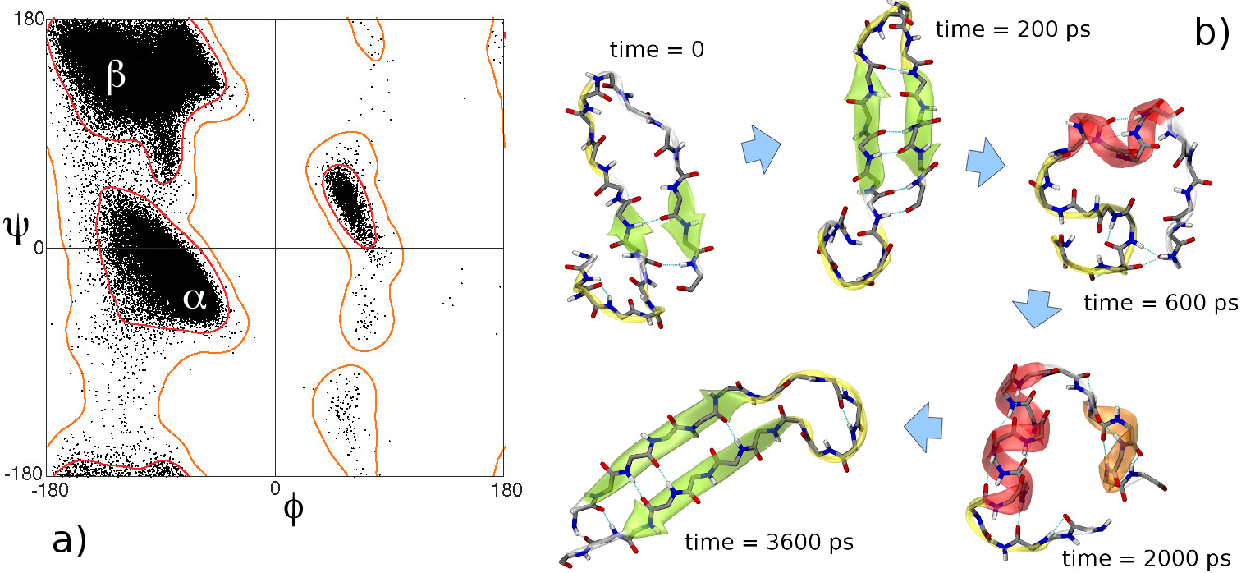
\includegraphics[width=13cm,angle=0]{./figures/secstr}
\caption{a) Ramachandran plot of backbone dihedral angles. 
b) structures explored during a simulation on the Val$_{20}$ peptide using the CVs {\tt ALPHARMSD} and {\tt ANTIBETARMSD}. 
}
\label{secstr}
\end{center}
\end{figure}

\subsection{{\tt ALPHABETA}}

This CV measures the (approximate) number of backbone dihedral angles which are similar to a given 
target angle~\cite{piana,piana08villin,todorova09}.
Each dihedral is specified by a set of four atom indexes followed by the target angle. Here we consider the $\psi$ dihedrals 
(which distinguish better than $\phi$ between alpha and beta) defined by atoms
(N$^1$-C$^1_\alpha$-C$^1$-N$^2$), and a reference value of -45$^\circ = -0.7854$~rad which corresponds to alpha helix.
The CV value ranges between 19 (the number of $\psi$ dihedrals in this example) when all $\psi=-45^\circ$, 
down to 0 when all $\psi=135^\circ$. Therefore the CV is able to switch between all-alpha and all-beta structures: 
in this example approximately 2~ns are needed for a complete loop, but estimating the FES would require
extended simulations due to the complexity of the conformational space of a 20-amino acid peptide
(i.e. the number of possible structures is very large).
%
\esempio{ Input for secondary structure exploration in a Val$_{20}$ peptide\\ \\
{\tt
\# 5 kJ/mol (gromacs units) every 5 ps (timestep = 2 fs)	\\
HILLS  HEIGHT 5.0  W\_STRIDE 2500			\\
PRINT W\_STRIDE 500					\\
\\
\# psi dihedrals: reference = -45 deg = -0.78540 rad	\\
ALPHABETA NDIH 19 SIGMA 1.0				\\
    7     9    21    23  -0.78540	\\
   23    25    37    39  -0.78540	\\
   39    41    53    55  -0.78540	\\
   55    57    69    71  -0.78540	\\
   71    73    85    87  -0.78540	\\
   87    89   101   103  -0.78540	\\
  103   105   117   119  -0.78540	\\
  119   121   133   135  -0.78540	\\
  135   137   149   151  -0.78540	\\
  151   153   165   167  -0.78540	\\
  167   169   181   183  -0.78540	\\
  183   185   197   199  -0.78540	\\
  199   201   213   215  -0.78540	\\
  215   217   229   231  -0.78540	\\
  231   233   245   247  -0.78540	\\
  247   249   261   263  -0.78540	\\
  263   265   277   279  -0.78540	\\
  279   281   293   295  -0.78540	\\
  295   297   309   311  -0.78540	\\
	\\
ENDMETA
}}	

\subsection{{\tt ALPHARMSD} and {\tt ANTIBETARMSD}}

This class of CVs counts the (approximate) number of 3+3-residue blocks which are
similar to the ideal alpha helix or beta sheet (i.e., to the average experimental
structures)~\cite{pietrucci09jctc}. The similarity with respect to the ideal secondary structure is estimated
by the root mean square deviation between the distance matrices among backbone
N, C$_\alpha$, C, O and C$_\beta$ atoms (this is equivalent to the root mean square
cartesian distance in ref~\cite{pietrucci09jctc}).
These CVs are more efficient than the dihedral-based {\tt ALPHABETA}
to observe the formation of beta sheets in explicit solvent simulations of larger proteins.
%
\esempio{ Input for secondary structure exploration in a Val$_{20}$ peptide\\ \\
{\tt
\# 5 kJ/mol (gromacs units) every 5 ps (timestep = 2 fs)				\\
HILLS  HEIGHT 5.0  W\_STRIDE 2500						\\
PRINT W\_STRIDE 500								\\
										\\
\# with gromacs4+domain decomp. it's important to use this:			\\
ALIGN\_ATOMS LIST <secstr>				\\
secstr->						\\
\#   N    CA     C     O    CB				\\
    7     9    21    22    11				\\
   23    25    37    38    27				\\
   39    41    53    54    43				\\
   55    57    69    70    59				\\
   71    73    85    86    75				\\
   87    89   101   102    91				\\
  103   105   117   118   107				\\
  119   121   133   134   123				\\
  135   137   149   150   139				\\
  151   153   165   166   155				\\
  167   169   181   182   171				\\
  183   185   197   198   187				\\
  199   201   213   214   203				\\
  215   217   229   230   219				\\
  231   233   245   246   235				\\
  247   249   261   262   251				\\
  263   265   277   278   267				\\
  279   281   293   294   283				\\
  295   297   309   310   299				\\
  311   313   325   326   315				\\
secstr<-						\\
							\\
\# 0.1 = conversion from nm (gromacs) to angstrom (internal reference structures)			\\
ALPHARMSD    LIST <secstr> SIGMA 0.3 R\_0 0.08 NN 8 MM 12 ANGSTROM\_SCALE 0.1 STRANDS\_CUTOFF 1. NOPBC	\\
													\\
ANTIBETARMSD LIST <secstr> SIGMA 0.3 R\_0 0.08 NN 8 MM 12 ANGSTROM\_SCALE 0.1 STRANDS\_CUTOFF 1. NOPBC	\\
													\\
ENDMETA													\\
}}
%
In the latter input file the {\tt R\_0}, {\tt NN}, {\tt MM} parameters are optimized to count $\sim 1$
only if the structure is similar to the ideal one, while {\tt STRANDS\_CUTOFF 1} limits the computation
of the CVs to protein segments which are not farther than 1~nm from each other, for efficiency, and
finally {\tt NOPBC} prevents the pairing of beta strands between periodic replicas of the protein (even
if in the present example the system is isolated, without pbc).
As a list of 20 residues is given in input, the CV measures the total content of alpha or antiparallel beta
secondary structure in the protein, without telling the specific position in the chain. Therefore e.g.
a value of {\tt ALPHARMSD} equal to 4 may correspond to a short helix at the beginning, at the center, or
at the end of the protein. By using several times the CVs for different chain segments it is possible
to localize the secondary structure in specific regions. 
In a few ns different secondary structure elements can be observed (Fig.~\ref{secstr}-b). 
Estimating the FES, as explained above for {\tt ALPHABETA}, 
would however require extended simulations due to the complexity of the conformational space.


\section{Potentials on a grid}

As the simulation goes on, the computational time spent in the evaluation of 
the metadynamics contribution to the forces becomes larger and larger and 
eventually comparable with the time needed to calculate the main forces in the MD code.
This effect is particularly visible when the system simulated is small or when using a simplified
coarse-grained potential.

A possible solution to this problem is storing an array containing the current value of the bias potential
(and of the derivatives with respect to the CVs) on a grid.
In this way the computational cost of metadynamics becomes constant during the simulation.
This corresponds to the cost of evaluating a single Gaussian function on the whole grid with a frequency given by the
stride between subsequent hills.

In order to activate the grid in \plumed, the directive \keyword{GRID} must be specified for every
collective variable {\tt CV}. The keyword  {\tt MIN} and {\tt MAX} are used to fix the CV interval, {\tt NBIN} the number of bins
and the flag {\tt PBC} if the CV is periodic.

In working with grids, we use the following conventions:
\begin{itemize}
\item the actual number of bins created is {\tt NBIN} + 1.
For example, if MIN is 0, MAX is 5 and NBIN is 5, the grid
is made by 6 bins: [0,1), [1,2), [2,3), [3,4), [4,5), [5,6).
\item a point is aligned to the left. 0.999 belongs to [0,1) and 
1.001 to [1,2). 
\end{itemize}

Special labels can be used in the definition of the interval with {\tt MIN} and {\tt MAX}, such
as {\tt -pi, +pi, +2pi, -2pi, pi, 2pi}. These labels may be particularly useful with the CVs {\tt ANGLE} or
{\tt TORSION}.

\esempio{In this example we run metadynamics using a dihedral angle as CV. 
The bias potential is put on a grid of 100 bins defined between $-\pi$ and $+\pi$. The grid is periodic. \vspace{10pt} \\
{\tt
HILLS W\_STRIDE 1000 HEIGHT 0.4\\
WELLTEMPERED SIMTEMP 300 BIASFACTOR 8\\
TORSION LIST 5 7 9 15 SIGMA 0.35\\
GRID CV 1 MIN -pi MAX +pi NBIN 100 PBC\\
ENDMETA
}}

As in standard metadynamics, a {\tt HILLS} file containing the list of Gaussians deposited is produced.
This file is needed to restart a metadynamics simulation also when \keyword{GRID} is used.
Alternatively, one can dump the grid of the potential on a file using the
keyword \keyword{WRITE\_GRID} and restart the simulation with \keyword{READ\_GRID} (see the manual).

Some rules to keep in mind:
\begin{itemize}
\item {\tt GRID} must be activated (or switched off) on ALL the CVs;
\item {\tt GRID} can be used together with multiple walkers metadynamics, bias-exchange and
      parallel tempering metadynamics;
\item For an accurate calculation of the potential and forces, the bin size must be smaller than
     half the Gaussian sigma. If a larger size is used, the code will stop.
\item If the simulation goes out of the grid, the code will stop. Please increase {\tt MIN} or {\tt MAX}
          and restart metadynamics.
\end{itemize}


\section{Reweighting techniques}

From a converged metadynamics run we can calculate directly the canonical probability distribution of the
collective variables at a given temperature.
On the contrary, the statistics of other degrees of freedom is somehow distorted by the application, 
during the simulation, of a time-dependent external potential on the CVs.
Different possible techniques have been proposed to reconstruct the probability distribution of variables other than the CVs.
Here we describe two of them.

\subsection{Well-tempered metadynamics calculations}

In WT metadynamics, the reconstruction of the distribution of variables different from the CVs
is particularly simple since for long times the amount of bias added decreases to zero and the
system becomes closer and closer to equilibrium.

The algorithm described in Ref. \cite{Bonomi:2009p17105} consists of three different steps:
\begin{enumerate}
\item Accumulate the histogram of the CVs plus the other variables of interest between
two updates of the bias potential;
\item When a new Gaussian is added, evolve the histogram following:
\begin{equation}
P(\bm{R},t+\Delta t)= e^{-\beta(\dot{V}(\bm{S}(\bm{R}),t)-\langle \dot{V}(\bm{S},t) \rangle )\Delta t} \, P(\bm{R},t),
\label{evol2}
\end{equation}
where $P(\bm{R},t)$ is the  biased probability distribution, $\dot{V}(\bm{S}(\bm{R}),t)$  
the time derivative of the bias potential and the average in the exponent is calculated in the biased ensemble;
\item At the end of the simulation, the unbiased distribution $P_B(\bm{R})$ can be recovered from the histogram collected 
by using a standard umbrella sampling reweighting:
\begin{equation}
P_B(\bm{R}) \propto e^{\beta V(\bm{S}(\bm{R}),t)} \cdot P(\bm{R},t). 
\end{equation}
\end{enumerate}

Starting from \plumed\ version 1.3, we will provide a code to perform this (and other) kind of reweighting procedure.
In this tutorial we are presenting a beta version of {\tt reweight}. 
Here is an example of typical usage.

\esempio{We performed a metadynamics run with 2 CVs and we are interested
in reconstructing the distribution of a third variable. \vspace{0.25cm} \\

{\tt
 reweight -colvar COLVAR -hills HILLS -ncv 2 -nvar 3 -stride 1 -fes 3 -temp 300 -welltemp 
 \vspace{0.25cm} \\
   \begin{tabular}{ l l }
 -hills      & HILLS  filename \\                        
 -colvar     & COLVAR filename \\                        
 -out        & FES    filename  \\                       
 -ncv        & number of variables in HILLS \\                
 -nvar       & number of variables in COLVAR  \\              
 -stride     & ratio between COLVAR and HILLS stride\\
 -fes        & ID of the variables for FES in output \\       
 -temp       & temperature in Kelvin \\                  
 -ngrid      & histogram grid dimension \\               
 -nreject    & discard initial steps \\                
 -timeout    & stride for FES printout \\               
 -pi         & ID of the variables with $[-\pi;\pi]$ periodicity \\
 -welltemp   & control for well-tempered metadynamics \\
 -kjoule     & energy in kjoule/mol \\ 
  \end{tabular} 
}}

The code needs two files with the same format of the \plumed\ {\tt HILLS} and {\tt COLVAR} files.
In the latter, the metadynamics CVs should appear in the first $d$ column followed by the
variables whose distribution one wants to reweight. The ratio between the stride in {\tt COLVAR}
and {\tt HILLS} must be constant and greater than 1. The more data you have for the histogram, the better.

Some important things to keep in mind:
\begin{itemize}
\item For the choice of the bin size, please follow the suggestions described in section \ref{fes-reconstr};
\item Eq. \ref{evol2} is exact. However, at the beginning of the simulation the
average of $\dot{V}(\bm{S}(\bm{R}),t)$ can be calculated only approximately.
Luckily, a possible initial error is recovered for long times. 
Alternatively, one could discard the first part of the trajectory using the {\tt -nreject} option.
Please always check that your results are robust to a discard of initial parts of the trajectory;
\item As for the calculation of the FES with {\tt sum\_hills}, remember to control the convergence
by plotting the reconstructed distribution at different times by using {\tt -timeout}; 
\end{itemize}

\subsection{Weighted-histogram analysis of bias-exchange simulations}\label{bewham}
%fabio

As explained in Section~\ref{bemeta}, a bias-exchange metadynamics simulation
consists in a number $N$ of replicas of the system, each one reconstructing a
one-dimensional free-energy profile along a different CV.
Instead of having only $N$ one-dimensional projections, it is much more insightful to know
the full $N$-dimensional free-energy landscape of the system, which may resolve all the
relevant minima and transition states. This can be achieved by combining the data from all the
bias-exchange replicas into a suitable weighted-histogram technique~\cite{marinelli-trpc09}.

The basic idea is the following: imagine to divide the $N$-dimensional CV-space into a grid of
small $N$-dimensional bins (Fig.~\ref{bewham-scheme}).
The probability of the states (= bins) visited along the trajectory
is not given by the Boltzmann equilibrium distribution because the simulation is affected by the bias potential.
Similarly to umbrella sampling, after filling time the equilibrium probability
of state $\alpha$ can be estimated as:
\begin{eqnarray}
 p^i_\alpha \approx \sum_{t\in\Omega^i_\alpha} e^{\beta(V^i(s^i_t)-f^i)}
\end{eqnarray}
where $i$ is the replica index, $\Omega^i_\alpha$ is the set of configurations of replica $i$
belonging to state $\alpha$, $s^i_t$ is the trajectory in CV-space, $V^i$ is the
bias potential (time-averaged after filling time), and $f^i$ is a shift constant.
Each replica which visited state $\alpha$ gives an estimate $p^i_\alpha$, and one can make
a weighted average of them to obtain the best overall probability $p_\alpha$:
\begin{eqnarray}
p_\alpha = C \sum_i \pi^i_\alpha p^i_\alpha
\end{eqnarray}
where $C$ is a normalization constant and the weights $\pi^i_\alpha$ are computed by minimizing
the statistical error: 
\begin{eqnarray}
\sigma^2(p^i_\alpha) = g \sum_{t\in\Omega^i_\alpha} e^{2\beta(V^i(s^i_t)-f^i)}\ \ ,\ \ \ \ 
\sigma^2(p_\alpha) = C^2  \sum_i (\pi^i_\alpha )^2 \sigma^2(p^i_\alpha)
\end{eqnarray}
\begin{eqnarray}
\pi^i_\alpha = \frac{e^{\beta(f^i-\bar V^i_\alpha)} }{ \sum_j e^{\beta(f^j-\bar V^j_\alpha)} }\ \ ,\ \ \ \ 
e^{\beta \bar V^i_\alpha} = \frac{ \sum_{t\in\Omega^i_\alpha} e^{2\beta V^i(s^i_t)} }{ \sum_{t'\in\Omega^i_\alpha} e^{\beta V^i(s^i_{t'})} }
\end{eqnarray}
where $g$ is the number of trajectory frames which are time-correlated and the shift constants $f^i$ are determined self-consistently
(see Ref.~\cite{marinelli-trpc09} for details).
Finally, the free energy is given by the usual formula $F_\alpha = -k_B T \log p_\alpha$. 
In this way, if the grid of bins is fine-grained, the (discretized) $N$-dimensional free-energy landscape is reconstructed.
A scheme of the whole procedure is reported in Fig.~\ref{bewham-scheme}.
%
\begin{figure}
\begin{center}
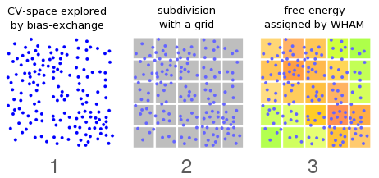
\includegraphics[width=11cm,angle=0]{./figures/bewham-scheme}
\caption{ The three steps of the bias-exchange + weighted histogram analysis method. }
\label{bewham-scheme}
\end{center}
\end{figure}

As an example we consider the trajectories and Plumed output files generated from the bias-exchange
simulation on Ala$_3$ in Section~\ref{bemeta}.
The simulation consisted of four replicas, therefore four atomic trajectories, and each one reconstructed
a one-dimensional free-energy profile along a different backbone dihedral $\psi_1$, $\phi_1$, $\psi_2$, or $\phi_2$.
To reconstruct the fully-detailed four-dimensional free-energy landscape we employ the VMD plugin 
{\tt bemeta\_analyzer.tcl}, developed by Xevi Biarnes and Alessandro Laio.
The plugin reads the files {\tt traj0-3.xtc}, {\tt COLVAR0-3}, and {\tt HILLS0-3}.
There must be a one-to-one correspondence between each trajectory file and CVs file, e.g., each frame in
{\tt traj0.xtc} must correspond to a line in {\tt COLVAR0} and viceversa.
The plugin needs also an input file {\tt cluster.in}:
%
\esempio{ file cluster.in for bemeta\_analyzer.tcl: \\
{\tt
KT 2.4943				\\
HILLS\_FILE   hills0  		\\
HILLS\_FILE   hills1  		\\
HILLS\_FILE   hills2  		\\
HILLS\_FILE   hills3  		\\
GRO\_FILE     start.gro			\\
COLVAR\_FILE colvar0 traj0.xtc 	\\
COLVAR\_FILE colvar1 traj1.xtc 	\\
COLVAR\_FILE colvar2 traj2.xtc 	\\
COLVAR\_FILE colvar3 traj3.xtc 	\\
TRAJ\_SKIP 1		 		\\
NCV 4					\\
CVGRID 1 -3.14159 3.14159 10 PERIODIC	\\
CVGRID 2 -3.14159 3.14159 10 PERIODIC	\\
CVGRID 3 -3.14159 3.14159 10 PERIODIC	\\
CVGRID 4 -3.14159 3.14159 10 PERIODIC	\\
ACTIVE 4 1 2 3 4			\\
T\_CLUSTER 500.				\\
T\_FILL    500.				\\
N\_MIN 1	\\
DELTA 4		\\
G\_CORR 1	\\
REPR "all" "Licorice" "Name" "Opaque" \\
}
}
In this example $k_BT=2.5$~kJ/mol, 
an initial structure is given ({\tt start.gro}), no frames are skipped ({\tt TRAJ\_SKIP 1}), the total number
of CVs is 4, for each CV a grid is defined by the minimum, maximum, and number of subdivisions (periodicity,
due to the nature of the dihedral CVs, is asked for), the indexes of the active (biased) CVs in the {\tt COLVAR}
files is given, the clustering and filling time are 500 ps and a preferred VMD representation is selected.
Further parameters are {\tt N\_MIN} (minimum number of visits of each bin to be considered reliable),
{\tt DELTA} (maximum allowed deviation between estimates of the free-energy profiles in the first and second half of
the trajectory), and {\tt G\_CORR} (number of time-correlated frames in the trajectory).

Finally, the plugin can be run from the TK console of VMD (open it from the "VMD Main" window,
clicking on Extensions, Tk console):
%
\esempio{ {\tt
source "bemeta\_analyzer.tcl" \\
::bemeta\_gui
}}
%
The input file {\tt cluster.in} is automatically read, and a graphical interface opens (see Fig.~\ref{bewham_gui}). 
%
\begin{figure}
\begin{center}
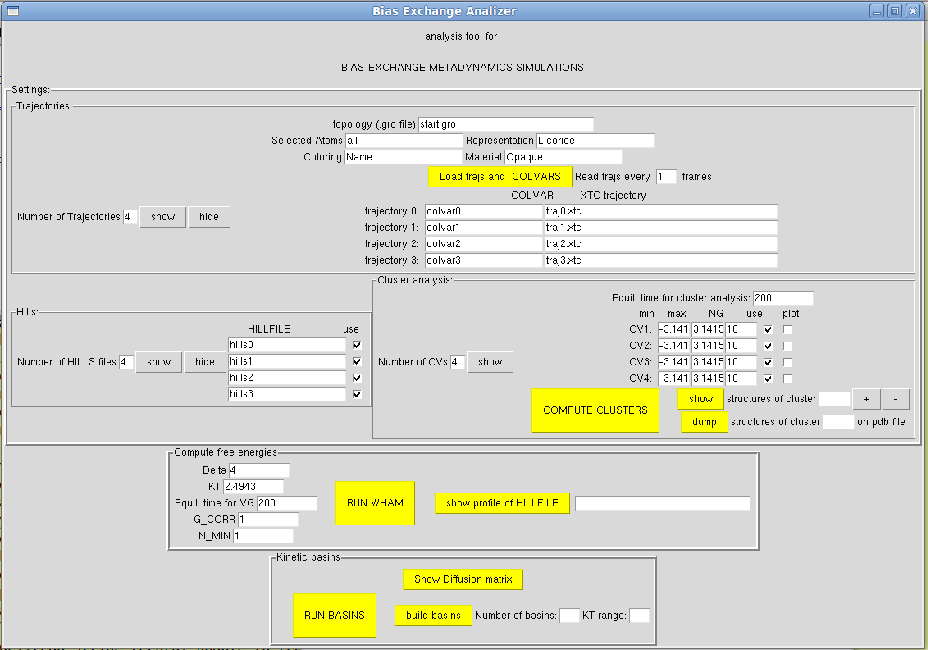
\includegraphics[width=14cm,angle=0]{./figures/bewham_gui}
\caption{ Graphical interface of the VMD plugin {\tt bemeta\_analyzer.tcl}. }
\label{bewham_gui}
\end{center}
\end{figure}



The following two commands load the data into VMD 
(trajectories and CVs). The fourth command subdivides the CV-space into a grid of bins and assigns each frame of the trajectory to a bin (or cluster). 
The last command calls the program {\tt wham\_on clusters\_newalign.x} which must be located in the same directory as all the input files. 
This program estimates the free-energy of each bin (or cluster) as explained above, writing it in the file CLUSTERS.FES:
%
\esempio{ the file CLUSTERS.FES: the columns are 1) the cluster index, 2) the population, 3,4,5,6) the 4 CVs 
defining the centre, and 7) the free energy\\
{\tt
1 \ \ 	 10 \ \  	 -2.61799 	 -2.61799	  0.52359	 -2.61799 \ \ \ \  10.173 \\
2 \ \  	 42 \ \ 	  1.57079 	 -1.5707	 -0.52359	 -1.57079 \ \ \ \  4.305  \\
3 \ \  	 35 \ \  	 -0.52359 	 -2.61799	 -0.52359	 -1.57079 \ \ \ \  5.224  \\
4 \ \  	 23 \ \  	 -0.52359 	 -2.61799	  0.52359	 -2.61799 \ \ \ \  7.183  \\
.....\\
}}
(note that some states may have a free energy of 1000: this means that due to poor statistics the
free energy could not be assigned, and probably it is very high).
This file contains therefore a discrete representation of the four-dimensional free-energy landscape
on a $10\times10\times10\times10$ grid. One can partially visualize the landscape, limited  e.g. to the 
two $\psi$ dihedrals, with gnuplot:
%
\esempio{{\tt
  set zrange [0:50] \\
  set xlabel "psi1" \\
  set ylabel "psi2" \\
  set zlabel "F (kJ/mol)" \\
  splot "CLUSTERS.FES" u 3:5:7
}}
%
or with other combinations (4:5:7, 5:6:7, 4:6:7, etc.).
The free-energy landscape can be compared with the one obtained from a long (3~$\mu$s) equilibrium MD simulation
(see Section~\ref{bemeta} and Fig.~\ref{be-validation}), in file {\tt EQUIL\_CLUSTERS.FES}. The script
{\tt compare\_clusters.sh} performs the comparison.
Note that the equilibrium MD has a poor sampling of the barrier regions, while metadynamics has a good sampling,
therefeore the agreement between {\tt EQUIL\_CLUSTERS.FES} and {\tt CLUSTERS.FES} deteriorates at high free energy.

The plugin {\tt bemeta\_analyzer.tcl} allows further to perform a kinetic clustering of the hundreds of states
in file {\tt CLUSTERS.FES}, by constructing an approximate kinetic transition matrix and analyzing its spectrum. 
This procedure locates the free-energy basins (i.e. significant local minima, each one including many states).
The detailed explanation of this procedure is beyond the scope of this tutorial, and the reader is referred to 
specific documentation. Only a rapid introduction is given here.
In short, the program {\tt kinetic\_basins.x} must be in the same directory, 
and the commands for {\tt bemeta\_analyzer.tcl} are the following:
%
\esempio{{\tt
run\_basins \\
build\_basins \\
show\_basins
}}
%
At this point VMD visualizes the clusterized structure of the CV-space, with basins as sets of small spheres of the same color,
and basin attractors (the centers of local free-energy minima) as bigger spheres. By clicking on the key "1" 
(picking mode) inside the VMD display, it becomes possible to select a state from the grid by left-clicking with the mouse.
The corresponding atomic configurations of Ala$_3$ then appear. To return to the CV-space representation it is sufficient
to click on "D" in the VMD Main window for the label "CLUSTERS.FES.BASINS".


\chapter{Inside PLUMED}
\section{How to plug PLUMED in your MD code}

In this part of the tutorial we will learn how to plug \plumed{} in
your MD code.

The usual manner to patch \plumed{} into a supported MD code is to use the
tools in the {\tt patches/} directory of \plumed{}.
These scripts are slightly modifying the host MD code by:
\begin{itemize}
\item changing the original Makefile so as to compile also plumed source
\item linking the plumed source code in the proper directory
\item adding proper calls to \plumed{} routines
\end{itemize}
The first two issues are very code dependent, and should be done in an ad-hoc
manner. We will focus here on the third issue.
To provide a working example, we will patch \plumed{} on a simple Lennard-Jones code
written in basic {\tt FORTRAN}.
So, as a first step get the {\tt simplemd.tgz} code. It contains a {\tt src}
directory with source code and a {\tt xyz} directory with input files.
Compile it and run it as follows
\esempio{
cd src \\
./compile \\
cd ../xyz \\
../src/simplmd.x $<$ in
}

The MD code needs to call \plumed{} routine for initialization (once at the beginning
of the simulation) and, at each step, to calculate the forces coming from the bias.
The two routines are {\tt mtd\_data\_init} and {\tt meta\_force\_calculation}.
Have a look to the {\tt common\_files/metadyn.c} file. You will find several versions
of these routines, depending on which host code is used. Instead
of adding new routines, we will just adapt the one used for AMBER.
The reason is that AMBER is also written in {\tt FORTRAN}, and its
interface is the simplest one.

We copy the plumed source in the {\tt src} directory
\esempio{
cp PLUMED-ROOT/common\_files/*.c {\tt src/}
cp PLUMED-ROOT/common\_files/metadyn.h {\tt src/}
}

We change the compile script in such a way to compile also plumed source.
Notice that we have to tell to plumed the name of the host MD code. For this
example, since we are using the AMBER interface, we add a
{\tt -DAMBER} compilation flag.
\esempio{
\# Compilation script: \\
gfortran -fdefault-real-8 -O2 -c *.f90 \\
gcc      -DPLUMED\_AMBER -O2 -c *.c \\
gfortran *.o -o simplemd.x -lm
}

At this point the code should compile without errors. Now we have to set the proper calls
to {\tt mtd\_data\_init} and {\tt meta\_force\_calculation}.

The first one should be called just after initialization. A good point for this code is
after velocity randomization
\esempio{
! velocities are randomized according to temperature \\
call randomize\_velocities(natoms,temperature,masses,velocities,idum) \\
\\
CALL init\_metadyn(natoms,tstep,masses,masses,1,1.0D0,"plumed.dat"//char(0))
}
Notice that the interface is a bit cluttered because it is designed so as
to be used from many MD codes (QuantumEspresso, AMBER and DLPOLY).
The first argument is the number of atoms, followed by the time-step, the array with the masses.
Then we should have the charges (we just set them equal to the masses since there are no charges
in LJ codes). The next argument indicates the type of pbc, followed by energy units, and by the
name of the plumed input (we leave it hardcoded to plumed.dat).

The call to plumed forces should be put just after the call to LJ forces:
\esempio{
  call compute\_forces(natoms,listsize,positions,cell,forcecutoff,point,list,forces,engconf) \\
  call meta\_force\_calculation(cell9,istep,positions,0,0,forces,0,0,engconf)
}
Notice here the two zeros following positions and forces. The reason is that the interface is
designed so as to be used also with DLPOLY, where three different arrays are passed (x, y and z components).





\section{How to add a new CV}

In this part of the tutorial we will learn how to add a new CV to \plumed.
Inside the code, every CV is identified by a unique name such as {\tt DISTANCE},
{\tt ANGLE} or {\tt TORSION} and by a numeric ID (see the manual for a list). 
In the following we will call the new CV using the keyword {\tt NEWCV} 
and use the ID {\tt 0} when needed. 

Adding a new CV to \plumed \ consists of three main steps: 
\begin{enumerate}
\item create a new file called {\tt restraint\_newCV.c}. This file will contain
all the routines needed to parse the \plumed \ input file and to calculate the value of {\tt NEWCV} 
and its derivatives with respect to the coordinates of the system;
\item modify the \plumed \ source code in a few places; 
\item reapply the patch and recompile your MD code.
\end{enumerate}

\subsection{Creating {\tt restraint\_newCV.c}}

Let's start by including the file that contains all the definition of routines and
variables that are probably needed, namely {\tt metadyn.h}.

\subsubsection{The parser}
The first important routine that must be defined in {\tt restraint\_newCV.c} is the parser, usually named {\tt read\_newCV}.
This routine will be called by \plumed \ when the main parser finds the keyword {\tt NEWCV} in the input file. 

As far as parsing is concerned, there are two main types of CVs.
The majority of them needs to read only one line from the input file.
An example is {\tt ANGLE}:
\vspace{0.25cm} \\
{\tt ANGLE LIST 11 13 17 SIGMA 0.35}\\

It should be noted that this CV may be defined also in terms of group of atoms, whose definition is
given in another place of the \plumed \ input file:
\vspace{0.25cm} \\
{\tt ANGLE LIST 11 13 <CA> SIGMA 0.35 \\
CA-> 3 7 10 CA<-} \\

The parser for this kind of CVs is declared as: 
\vspace{0.25cm} \\
{\tt int  read\_angle  (char **word,int count,t\_plumed\_input *input,           FILE *fplog);}\\

where:
\begin{itemize}
\item {\tt **word} contains the entire line of the input file that starts with {\tt ANGLE}; 
\item {\tt count} is a CV counter;
\item {\tt *input} is a complex structure which contains all the \plumed \ input file;
\item {\tt *fplog}  points to the \plumed \ log file.
\end{itemize}

A few CVs need to read from the input file data with a syntax different from groups of atoms.
To do so, we need to pass an additional information to the parser. 
An example is {\tt RMSDTOR}. This CV needs to scan the input file for a list of atoms that defines
a dihedral angle and to read a reference value:
\vspace{0.25cm} \\
{\tt RMSDTOR NDIH 2 SIGMA 0.35 \\
13 15 17 1 0.5 \\
15 17 1 3 2.0} \\

The parser for this kind of CVs is declared as:
\vspace{0.25cm} \\
{\tt  int  read\_rmsdtor       (char **word,int count,t\_plumed\_input *input,int *iline,FILE *fplog);} \\

where {\tt *iline} indicates the line of the input file that is currently parsed. 
This variable is modified when scanning the rest of the input file to 
get the additional data required by the CV. 

Here we will focus on the first type of CVs. In the example box below we show the essential lines of
the {\tt ANGLE} parsing routine.

\esempio{Structure of a typical parsing routine. \vspace{0.5cm} \\
 {\tt int PREFIX read\_angle(char **word, int count, t\_plumed\_input *input, FILE *fplog)\{ \vspace{0.2cm} \\
  int j, iw; \\
  double delta = 0.0; \vspace{0.2cm} \\

  iw = seek\_word(word,"LIST"); \\
  if(iw>=0) \{ \\
             j=plumed\_get\_group(word[iw+1],\&colvar.cvatoms[count],colvar.natoms[count],input,fplog); \\
             colvar.natoms[count]+=j; \\
             colvar.list[count][0]=j; \\
             j=plumed\_get\_group(word[iw+2],\&colvar.cvatoms[count],colvar.natoms[count],input,fplog); \\
             colvar.natoms[count]+=j; \\
             colvar.list[count][1]=j; \\
             j=plumed\_get\_group(word[iw+3],\&colvar.cvatoms[count],colvar.natoms[count],input,fplog); \\
             colvar.natoms[count]+=j; \\
             colvar.list[count][2]=j; \\
  \} else \{ fprintf(fplog,"|- NEEDED LIST KEYWORD FOR ANGLE");\} \vspace{0.2cm} \\

  iw=seek\_word(word,"SIGMA"); \\
  if(iw>=0)\{ sscanf(word[iw+1],"\%lf", \&delta); \\
             colvar.delta\_r[count]  = (real) delta; \} \vspace{0.2cm} \\ 
  
  colvar.type\_s[count]   = 4; \vspace{0.2cm} \\

  snew(colvar.myder[count], colvar.natoms[count]); \vspace{0.2cm} \\

  return colvar.natoms[count]; \\
\}

}}

The example above shows some of the fundamental variables and routines that are used in the parser:
\begin{itemize}
\item {\tt seek\_word} looks for specific words in the parsed line;
\item {\tt plumed\_get\_group} is used to read a group of atoms;
\item {\tt colvar.natoms} is the total number of atoms  used to define this CV; 
\item {\tt colvar.cvatoms} is the list of atoms used to define this CV; 
\item {\tt colvar.delta\_r} is the Gaussian sigma;
\item {\tt colvar.type\_s} is the unique ID of the CV;
\item {\tt colvar.myder} will contain the derivatives of this CV with respect to the coordinates of
the atoms and must be initialized in the parser routine.
\end{itemize}

\subsubsection{CV definition and derivatives}

The second important routine that must be included in {\tt restraint\_newCV.c}
contains the mathematical definition of the CV and its derivatives and it is usually called {\tt newCV\_restraint}. 
The declaration of this routine is common among all the CVs. Below is the example 
of the {\tt ANGLE} restraint. 

\esempio{{\tt  void angle\_restraint         (int i\_c, struct mtd\_data\_s *mtd\_data);}}

The variables that appear in the declaration of {\tt newCV\_restraint} are:
\begin{itemize}
\item {\tt i\_c}, a CV counter;
\item {\tt *mtd\_data}, the fundamental structure of \plumed \ that contains data
passed from the main MD code. These include positions, masses and charges of all the atoms,
information about the time steps, temperature, unit of measure, periodic boundary conditions and others.  
\end{itemize} 

The routine {\tt newCV\_restraint} uses the information in {\tt mtd\_data} 
to calculate at every MD step the value of {\tt NEWCV} and to store it in the {\tt colvar.ss0[i\_c]} variable. 
The derivatives with respect to all the atoms involved must be also calculated and stored
in the {\tt colvar.myder} array.

\subsection{Modifying the \plumed \ source code}

Once the routines for parsing the new CV and calculating its value and derivatives
have been implemented, we need to modify the source code to instruct \plumed \ to call them at the right moment.  
To do so, we have to act in a few selected spots:
\begin{enumerate}
\item we have to add the declaration of the new routines {\tt read\_newCV} and {\tt newCV\_restraint}
in the {\tt metadyn.h} file;
\item in the {\tt read\_restraint.c} file, we have to tell \plumed \ to call {\tt read\_newCV} when
the keyword {\tt NEWCV} is found in the input file. Here are the relevant lines for the {\tt ANGLE} CV:
\vspace{0.25cm} \\
{\tt     \} else if(!strcmp(word[0],"ANGLE"))\{ \\
      read\_angle(word, count, \&input, mtd\_data->fplog); \\
      count++; \\ \} }
\item in the {\tt restraint.c} file, we have to tell \plumed \ to call {\tt newCV\_restraint} when appropriate.
In the usual example of {\tt ANGLE} CV, whose ID is 4:
\vspace{0.25cm} \\
 {\tt switch(colvar.type\_s[i\_c])\{ \\
      ... \\
      case 4: angle\_restraint(i\_c, mtd\_data); break;         \\
      ... \\ \} }
\end{enumerate}
 

\subsection{Final steps}

Once the modifications to the \plumed \ source code are done, 
we need to reapply the patch and recompile the MD host code.
After that, we are ready to use our new CV. 

Before starting a real calculation, it is better to check that we have done everything correctly.
The most frequent source of error is the implementation of the analytical derivatives of the
CV with respect to the coordinates of the system. To detect possible errors, we can use the
keyword {\tt DEBUG}. Before doing so, we have to manually add
{\tt NEWCV} to the list of variables for which debugging is active. 
This list is defined in the file {\tt testderivatives.c} together
with the routines for comparing the analytical derivatives of a CV to the value calculated with 
finite differences. These routines call 
{\tt newCV\_restraint} several times to calculate the CV value for different atoms positions.
Have a look at {\tt testderivatives.c} and add all the calls to {\tt newCV\_restraint} that are needed,
following the usual example of {\tt angle\_restraint}! 


\chapter{Real life applications}

\section{The Stone-Wales transformation in a carbon nanotube}
%fabio

As an example of an activated process in a condensed matter system we consider
the Stone-Wales transformation in a carbon nanotube. This transformation
can be seen as the rotation of a C-C dimer by 90$^\circ$, which leads
to the conversion of four hexagons into two pentagons and two heptagons.
During the process, which has been observed e.g. in nanotubes subject
to strain, overall two covalent bonds are broken and two are formed, resulting
in a large energy barrier of several eV.
Here we consider a 480-atoms (10,0) carbon nanotube periodically repeated,
and we adopt the AIREBO interatomic potential as implemented in lammps.
One can imagine different suitable reaction coordinates for the Stone-Wales
transformation. Here we use the number of covalent three-atoms bridges 
among different groups of atoms, as detailed in Fig.~\ref{stone-wales}.
Rotation of the C-C dimer leads to breaking of two "vertical" bridges
and to forming two "horizontal" bridges. A suitable Plumed CV is
{\tt WATERBRIDGE} (the name water has only historical sense since the CV
was originally implemented to count the H-bonded bridges formed by water
molecules between two protein surfaces).
%
\esempio{ input file for the Stone-Wales transformation in a carbon nanotube with lammps \\ \\
{\tt
\# 0.4 eV (lammps "metal" units) every 50 fs (timestep = 1 fs) 	\\
HILLS HEIGHT 0.4 W\_STRIDE 50					\\
PRINT W\_STRIDE 10						\\
\\
WATERBRIDGE LIST <hor1> <hor2> <dimer> R\_0 1.9 NN 8 MM 20 SIGMA 0.2	\\
hor1->		\\
  229 259	\\
hor1<-		\\
hor2->		\\
  226 256	\\
hor2<-		\\
dimer->		\\
  238 248	\\
dimer<-		\\
\\
WATERBRIDGE LIST <ver1> <ver2> <dimer> R\_0 1.9 NN 8 MM 20 SIGMA 0.2	\\
ver1->		\\
  256 259	\\
ver1<-		\\
ver2->		\\
  226 229	\\
ver2<-		\\
\\
ENDMETA		
}}

\begin{figure}
\begin{center}
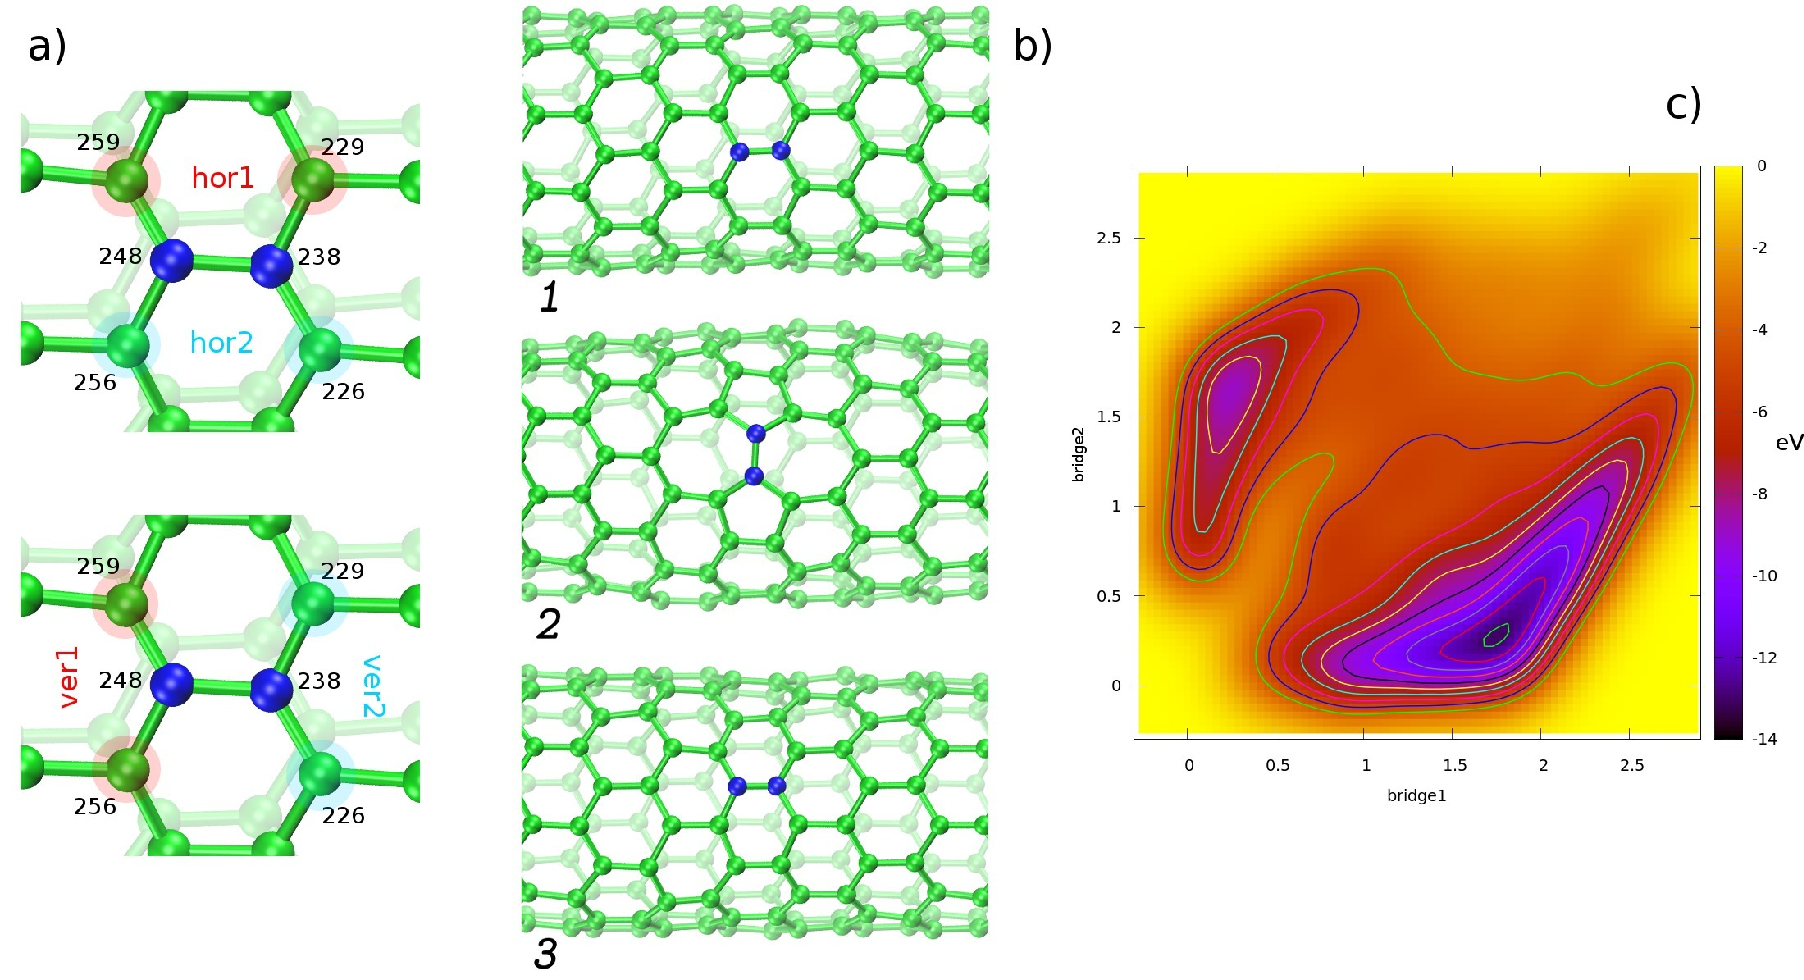
\includegraphics[width=14cm,angle=0]{./figures/stone-wales}
\caption{ a) Definition of the groups of atoms in the input file. b) Reversible Stone-Wales transformation during the simulation 
 with the CV {\tt WATERBRIDGE}. c) reconstructed FES after deposition of 400 hills. }
\label{stone-wales}
\end{center}
\end{figure}

Within 10~ps of simulation, the Stone-Wales transformation occurs reversibly
multiple times, and a FES can be reconstructed with {\tt sum\_hills}:
%
\esempio{
generate FES file fes.dat:\\
{\tt
sum\_hills.x -file HILLS -out fes.dat -ndim 2 -ndw 1 2\\
}
\\
plot FES with gnuplot:\\
{\tt
set pm3d\\
set contour base\\
splot 'fes.dat' with pm3d
}}

\section{A SN2 reaction in vacuum with quantum espresso}
This section will show a simple chemical reaction example done with QUANTUM ESPRESSO  code.
This code is meant here to do Born-Oppenheimer dynamics but \plumed\ is also  
implemented to work in the Car-Parrinello module of the suite.
The goal of the exercise is to calculate the free energy for the reaction depicted in \ref{sn2}.
This reaction has been studied before \cite{Yang:2004p15845} and here we will
try to sketch out the barriers but the aim is to take a short amount of time.
\begin{figure}
\begin{center}
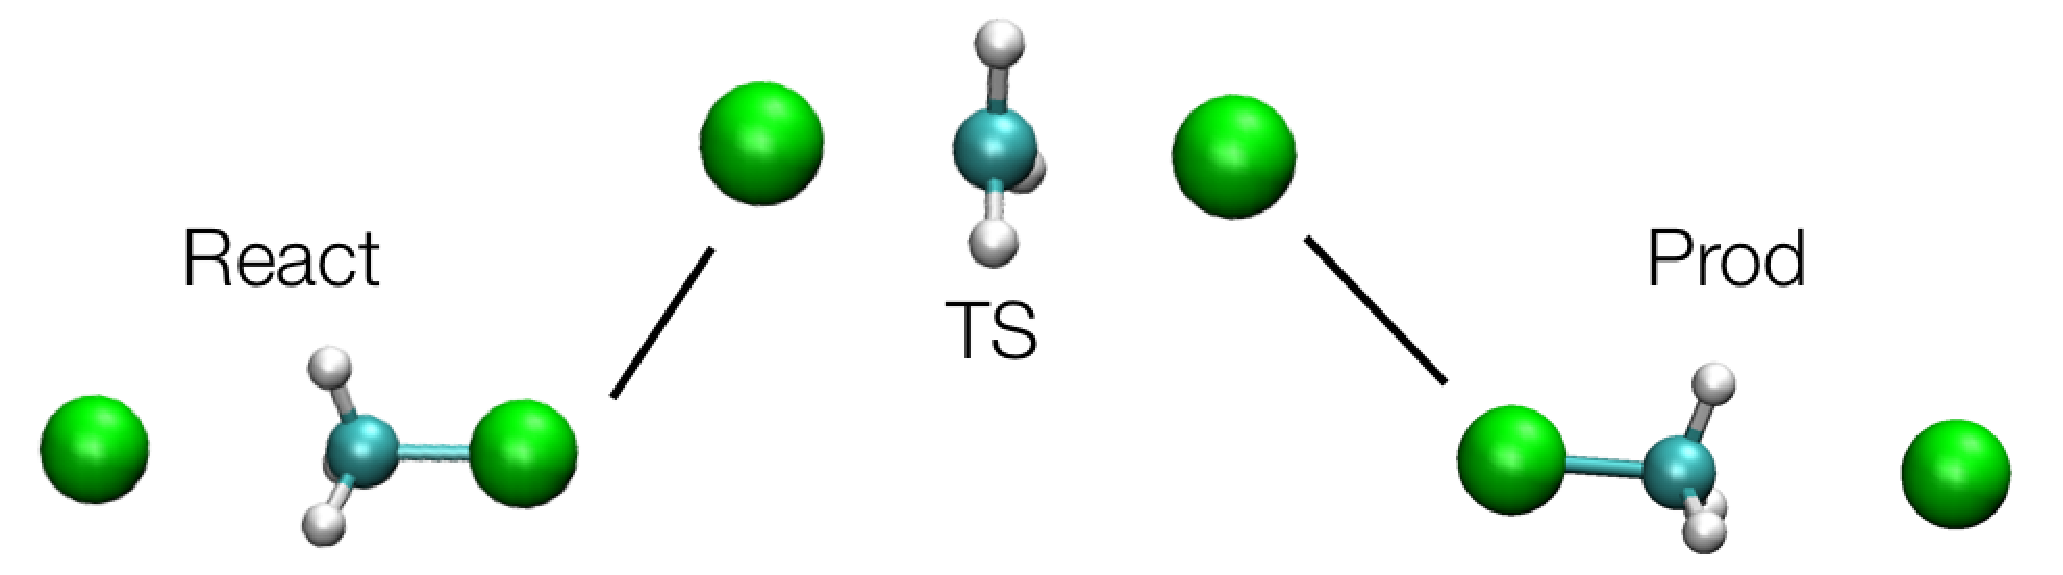
\includegraphics[width=14cm,angle=0]{./figures/sn2}
\caption{A sketch of SN2 reaction}
\label{sn2}
\end{center}
\end{figure} 
In the PW code input (file {\tt bo.in}) \plumed\ is activated with the flag {\tt use\_plumed=.true.} in the control section then 
the code expects a {\tt plumed.dat} file.
\begin{verbatim}
&control
    title = 'ch3cl',
    calculation='md'
    restart_mode='from_scratch',
    pseudo_dir = '.',
    outdir='.',
    dt=20,
    nstep=2000,
    disk_io='low',
    prefix = 'md',
    use_plumed = .true.,
 /
\end{verbatim}
Pay attention: in this code distances are in Bohr (1 Bohr = 0.529177249 {\rm \AA}) and the energies in Rydberg ( 1 Ry=  313.755 kcal/mol ).

Now you have to choose what to do at this stage. You have first a bunch of techniques available.
\begin{itemize}
\item Metadynamics? Can be an option but you have a fixed small amount of time available here. 
And you don't know how much it will take to make a  single event but you also might have multiple recrossing.
\item Thermodynamic integration (In the steered-md flavour). Efficient and guaranteed to make the reaction but no average on multiple recrossing events. And what about the dissipative work? Here you don't have many orthogonal degrees of freedom. Probably could work.
\item Umbrella Sampling. Similar problems to TI, with the exception that the work are calculated at equilibrium. No problem with dissipative work.
\end{itemize}
And the second thing that you should decide is the CV to be used.
\begin{itemize}
\item Distances?
\item Path ? (probably is overshooting?
\item Does the angle matters?
\item Coordination number?
\item Anything else?
\end{itemize}
For Metadynamics a possible input can be 
\esempio{
{\tt
\# switching on metadynamics and Gaussian parameters \\
HILLS HEIGHT 0.001 W\_STRIDE 2 \\
\# instruction for CVs printout\\
PRINT W\_STRIDE 1\\
\# the distance between C-Cl' and C-Cl\\
DISTANCE LIST 1 3 SIGMA 0.3\\
DISTANCE LIST 2 3 SIGMA 0.3\\
\#WALLS: prevent to depart the two mols\\
UWALL CV 1 LIMIT 7.0 KAPPA 100.0\\
LWALL CV 1 LIMIT 2.5 KAPPA 100.0\\
UWALL CV 2 LIMIT 7.0 KAPPA 100.0\\
LWALL CV 2 LIMIT 2.5 KAPPA 100.0\\
\# end of the input\\
ENDMETA
}}
Here two independent variable on a range are used.
A possible other input (case of steered md):
\esempio{
{\tt
\# instruction for CVs printout \\
PRINT W\_STRIDE 1\\
\# the distance between C-Cl' and C-Cl \\
DISTANCE LIST 1 3 DIFFDIST 2 3 \\
STEER CV 1 TO 2.35 VEL 2.50 KAPPA 0.5  \\
\# end of the input \\
ENDMETA
}}
\esempio{
{\tt
\# instruction for CVs printout \\
PRINT W\_STRIDE 1\\
\# the distance between C-Cl' and C-Cl \\
DISTANCE LIST 1 3 DIFFDIST 2 3 \\
DISTANCE LIST 1 2 \\
STEER CV 1 TO 2.35 VEL 2.50 KAPPA 0.5  \\
UWALL CV 2 LIMIT 8.7 KAPPA 0.5 \\
\# end of the input \\
ENDMETA
}}
In this other option you use one single cv and you keep a wall on the other.
Which are the advantages/disadvantages?
One variable is faster but you don't know where and how much the wall is affecting your
simulation. Is there any way to calculate and address this issue?
You can run the job like this
\begin{verbatim}
source  /usr/local/Modules/3.2.6/init/bash
module load intel-cc/10.1.015 
module load intel-fc/10.1.015
module load intel-mkl/10.0.1.014
module load openmpi/1.2.6_intel-10.1.015
PATH_TO_ESPRESSO=/my/path/to/espresso
mpirun -np 4 $PATH_TO_ESPRESSO/espresso-4.2.1/PW/pw.x < bo.in > bo.out
\end{verbatim}
Choose one of those two technique and run the calculation.
Use {\tt sum\_hills} or the awk script to calculate the work (in the steering example) to 
calculate the energy profile. 

\clearpage
\section{Folding of the GB1 C-terminal $\beta$--hairpin}
In this part of the tutorial, we will use \plumed \ in combination
with GROMACS to study the folding process of a small peptide, the
C-terminal domain of protein GB1 \cite{Serrano, eaton1}. This 16-residue peptide is a prototypical
example of $\beta$--hairpin structure (see Fig. \ref{hpin}) which has attracted the attention
of both the experimental and theoretical community in the recent years.

\begin{figure}[!h]
\begin{center}
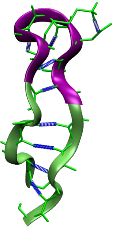
\includegraphics[width=2in,angle=0]{./figures/hpin}
\caption{Structure of the C-terminal domain of protein GB1. In violet, the residues
that define the turn region.}
\label{hpin}
\end{center}
\end{figure}

A variety of computational methods and models for the protein and the water force fields,
together with a number of different
 descriptors have been used in those works
aimed at characterizing the folding landscape of this peptide \cite{Pande2,dinn+99pnas,zhou+01pnas,
garc-sanb01prot,PTmetaD,Yoda2007,Bo.Bra:08,Best:2010p18495}. In particular, among the CVs used are: 
\begin{itemize}
\item Number of hydrogen-bonds;
\item Backbone radius of gyration;
\item Hydrophobic core radius of gyration;
\item RMSD;
\item ASA;
\item Principal components;
\item Path Collective Variables;
\item Contact maps.
\end{itemize}

In this exercise, we will experiment with different collective variables and free-energy methods.
We will simulate the hairpin in vacuum using the OPLS-AA \cite{opls_protein} force field. 
More precisely, in this exercise you should combine many of the techniques 
learnt in this tutorial and:

\begin{enumerate}
\item Choose a limited number of CVs;
\item Choose a free-energy method;
\item Restrict the turn region to simplify the problem; 
\item Monitor the RMSD of the protein from the native state to
see if the peptide is correctly refolding;
\item Monitor the convergence of your calculation;
\item Calculate and analize the FES.
\end{enumerate}

Here is an example of \plumed \ input file with some of the CVs that can
be used to address this problem. 

\esempio{
{\tt
PRINT W\_STRIDE 500 \\
\# choose your free-energy method\\
HILLS W\_STRIDE 500 HEIGHT 0.2\\

\# if you choose metadynamics, try to use GRID\\
\# GRID CV 1 MIN 0 MAX 10 NBIN 100\\

\# CHOOSE YOUR CVs or create your own\\
\# number of native CA contacts\\
CMAP INDEX CMAP\_native.CA \\

\# total number of CA contacts \\
CMAP INDEX CMAP\_all.CA  \\

\# RMSD**2 from native structure calculated on CA \\
TARGETED TYPE RMSD FRAMESET hpin\_native\_CA.pdb \\

\# RMSD**2 from native structure calculated on backbone \\
TARGETED TYPE RMSD FRAMESET hpin\_native\_BACKBONE.pdb \\

\# number of hbonds \\
\# TYPE means \\
\# 0  ALL  \\
\# 1  BETA ODD \\
\# 2  ALPHA \\
\# 3  BETA EVEN \\ 
\# 4  NATIVE (like PAIR coordination) \\
\# 5  BETA ALL \\
HBONDS LIST <H> <O> TYPE 1 \\
H-> \\
15  30  54  68  89  101  113  123  137  159  173  193  207  223 \\
H<- \\
O-> \\
28  52  66  87  99  111  121  135  157  171  191  205  221  235 \\
O<- \\

\# radius of gyration of the hydrophobic core \\
RGYR LIST <HC>  \\
HC-> \\
29  31  33  36  37  39  40  42  43  45  47  49  51  52 \\
67  69  71  74  75  77  79  81  83  84  86  87  172  174  176  179  180 \\
182  184  186  188  190  191  206  208  210  212  216  220  221 \\
HC<- \\

\# CA radius of gyration \\
RGYR LIST <CA>  \\
CA-> \\
9  16  31  55  69  90  102  114   \\
124  138  160  174  194  208  224  238 \\
CA<- \\

\# you may want to keep the turn formed \\
TARGETED TYPE RMSD FRAMESET hpin\_native\_TURN.pdb \\
UWALL CV 2 LIMIT 0.01 KAPPA 5000000.0 EXP 2.0 \\

ENDMETA \\

}}


\clearpage



\bibliographystyle{./elsarticle-num}
%\phantomsection
%\addcontentsline{toc}{chapter}{Bibliography}
\bibliography{../manual/bibliography}
\printindex

\end{document}
